\chapter*{Appendix B: Hadronic recoil reconstruction using MVA}
\addcontentsline{toc}{chapter}{Appendix B: Hadronic recoil reconstruction using MVA}
\markboth{Appendix B: Hadronic recoil reconstruction using MVA}{}
    Current appendix contains the comparison of all the kinematic distributions for all W and Z channels.
    
    \begin{figure}[h]
    	\centering
    	{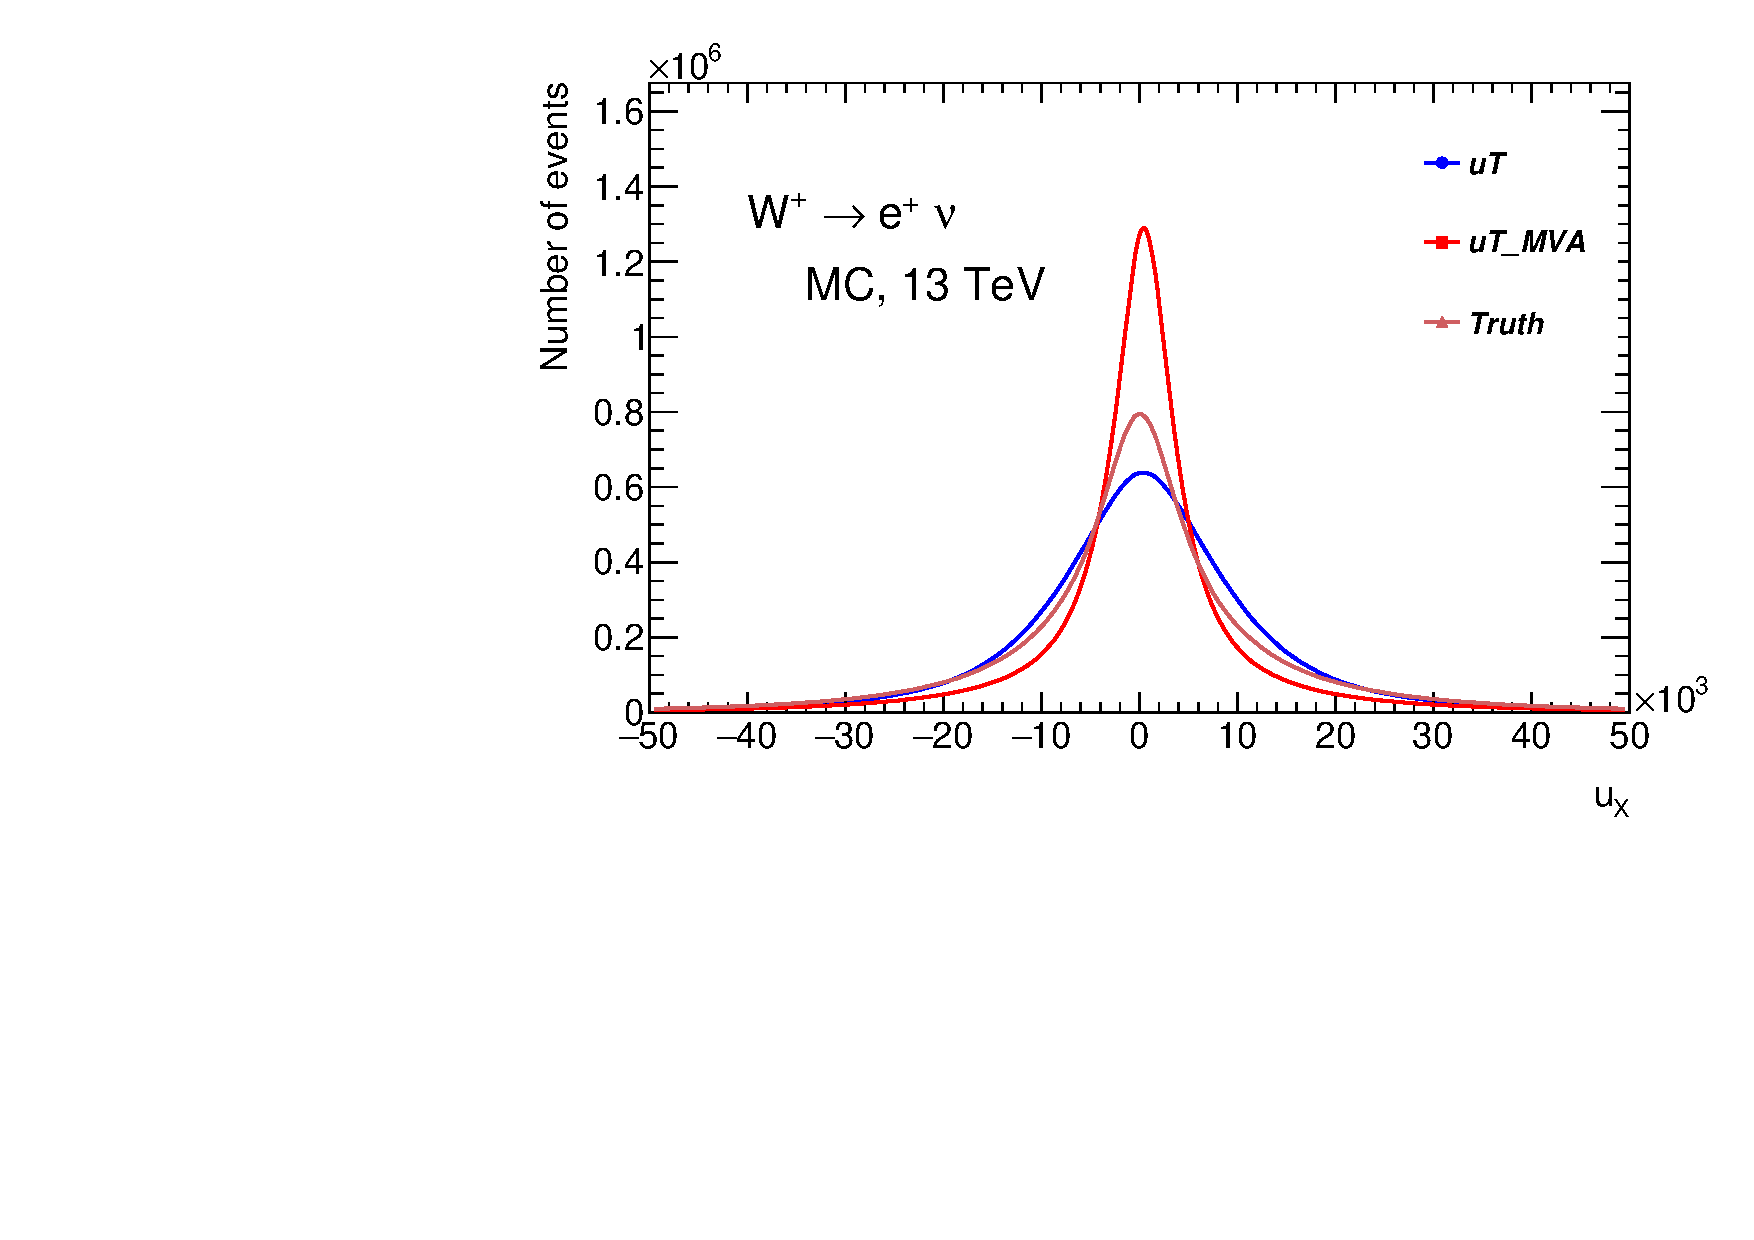
\includegraphics[width=.49\textwidth]{hist_uXplusenu.pdf}}
    	{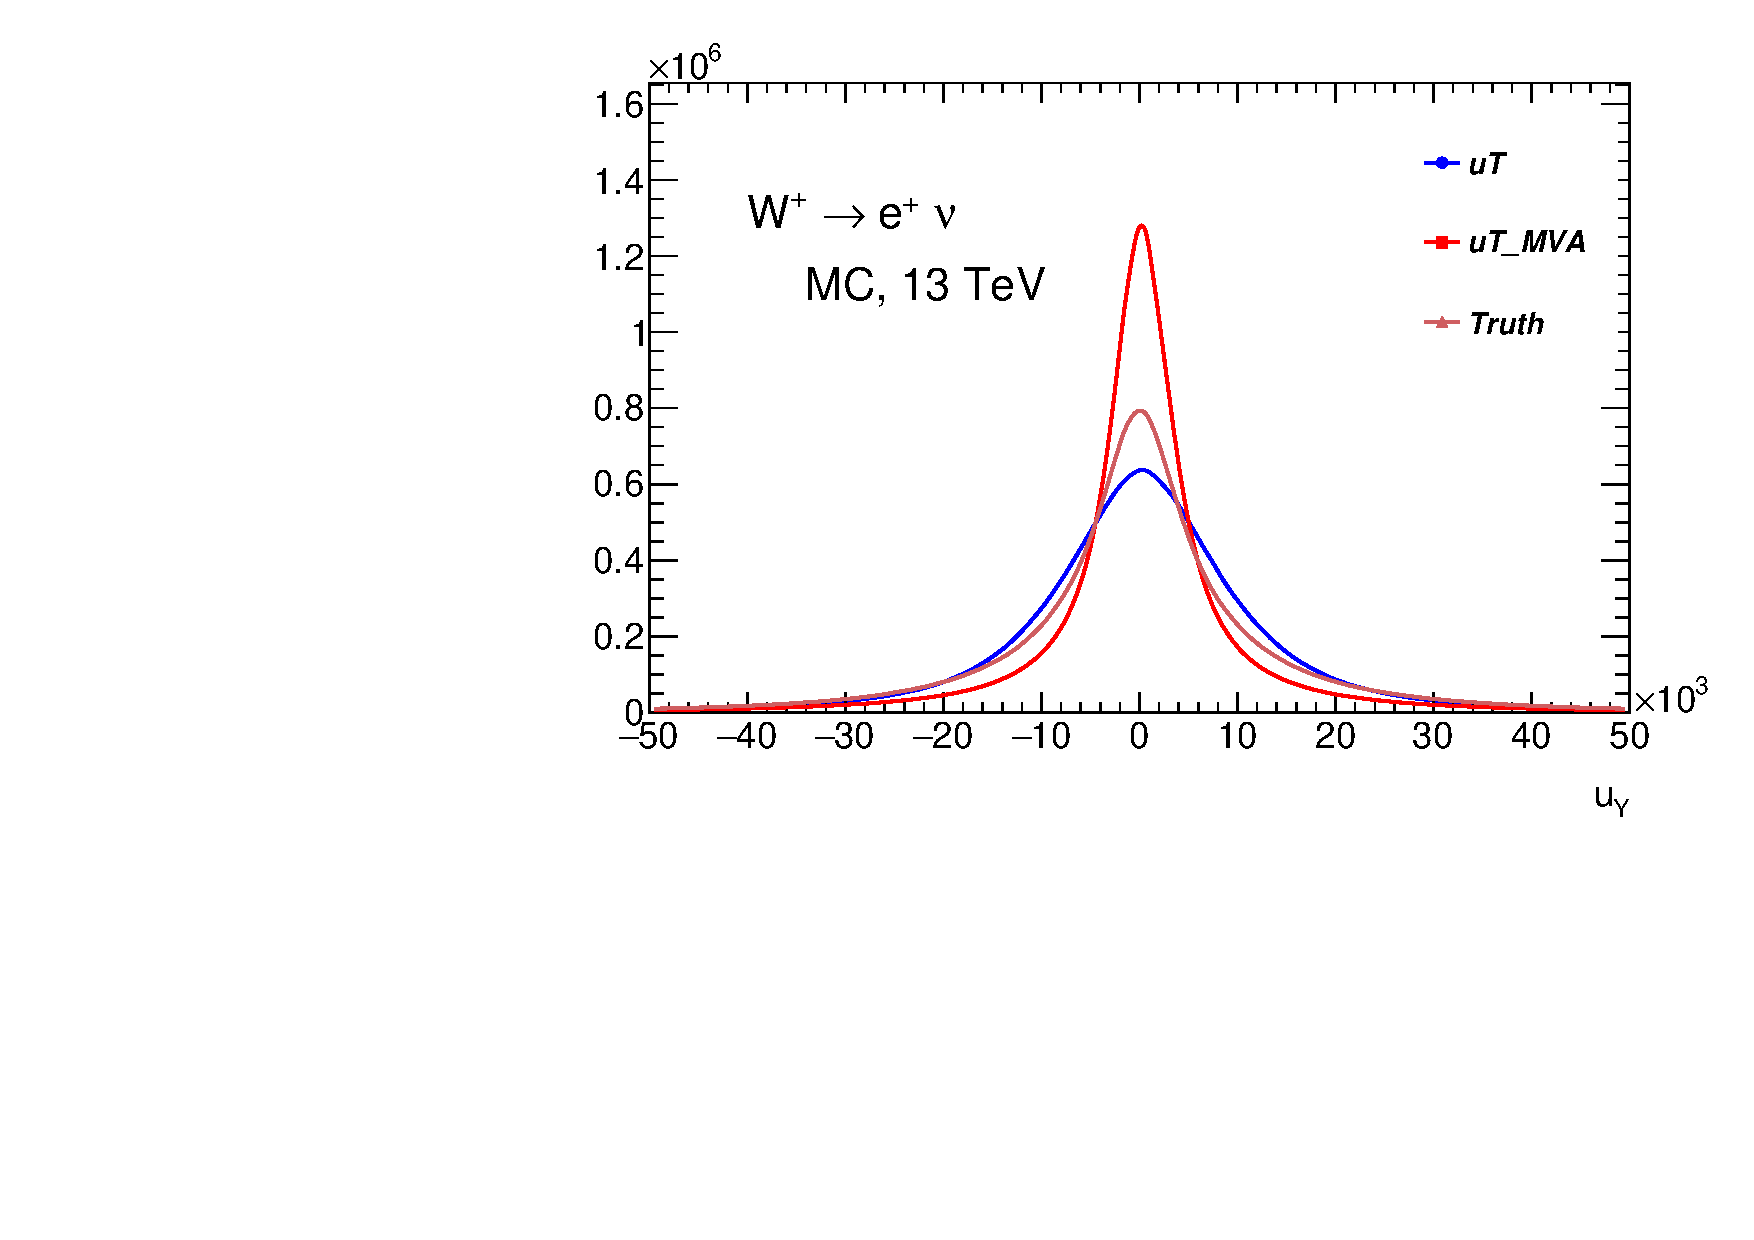
\includegraphics[width=.49\textwidth]{hist_uYplusenu.pdf}} \\
    	{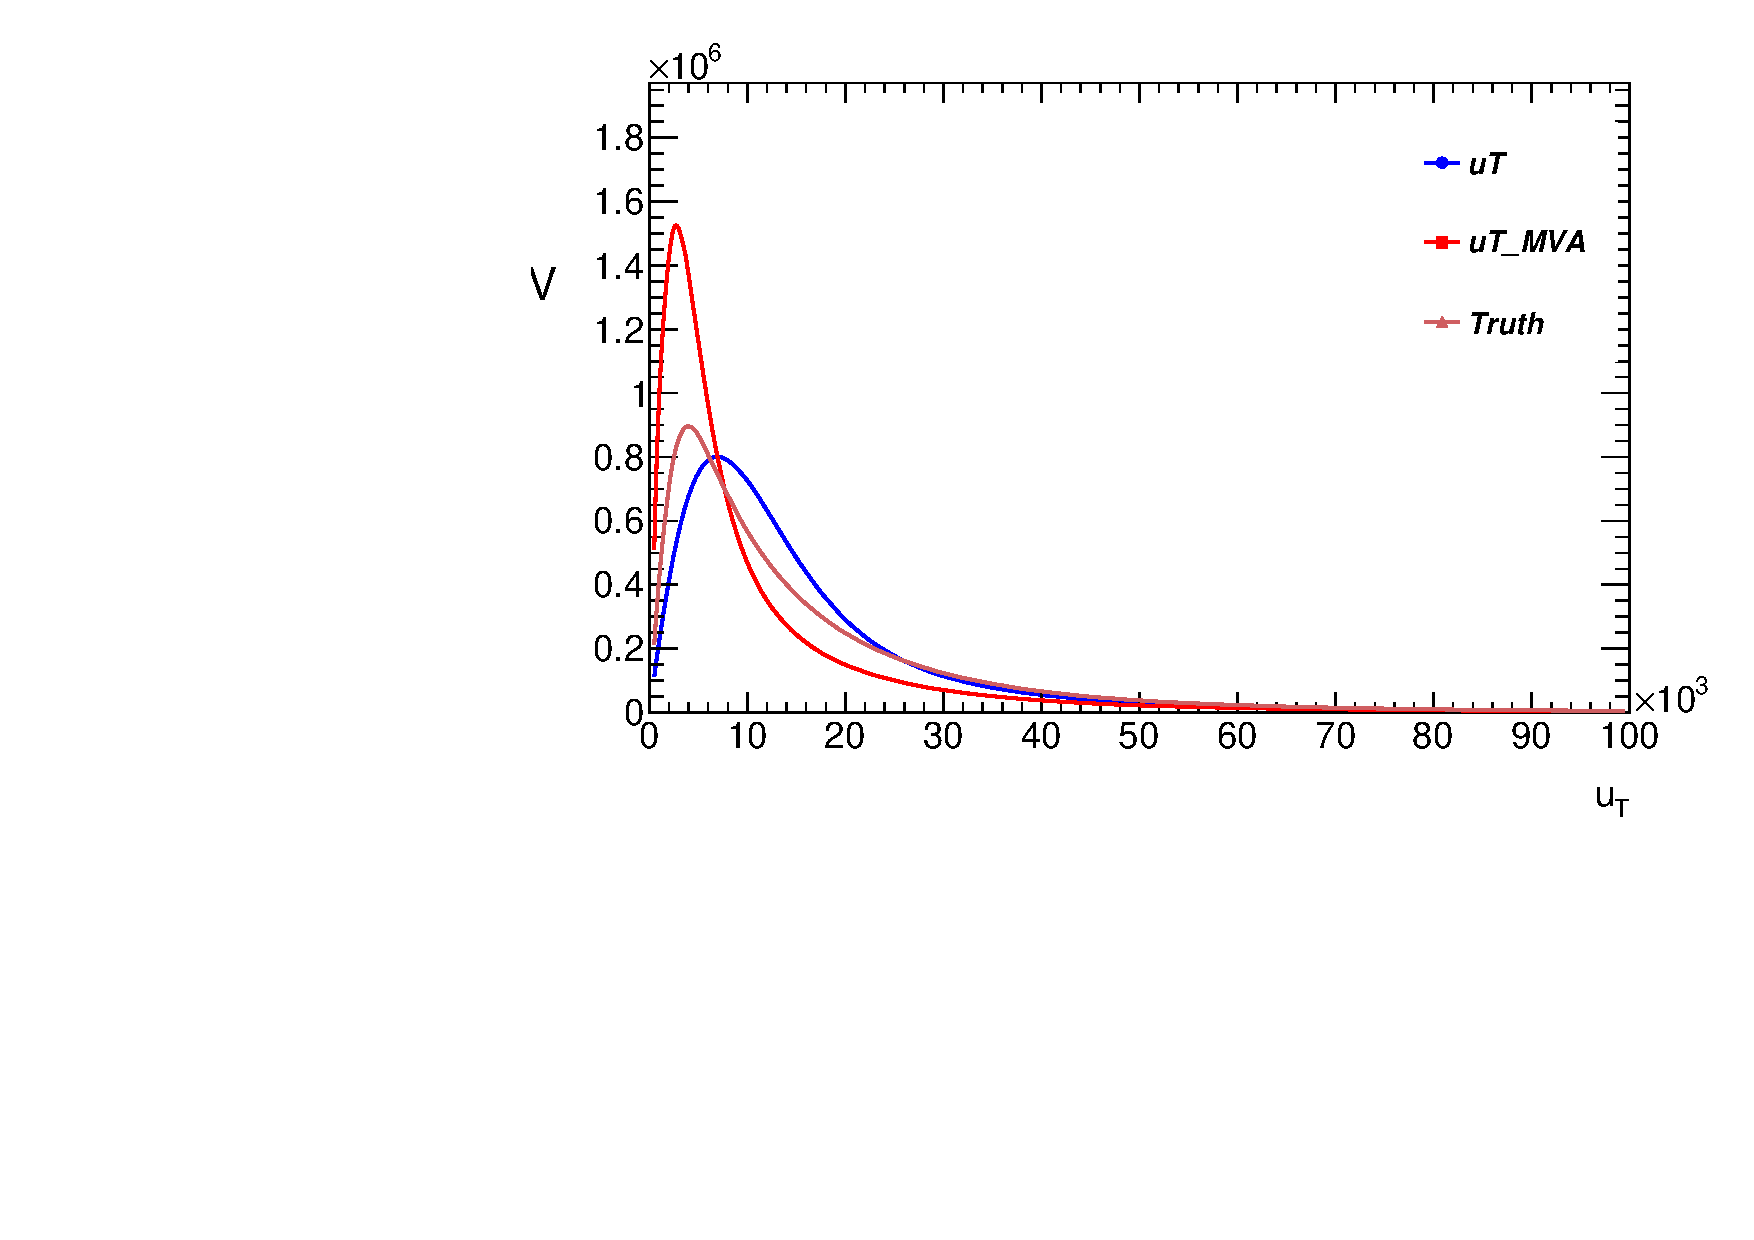
\includegraphics[width=.49\textwidth]{hist_uTplusenu.pdf}}
    	{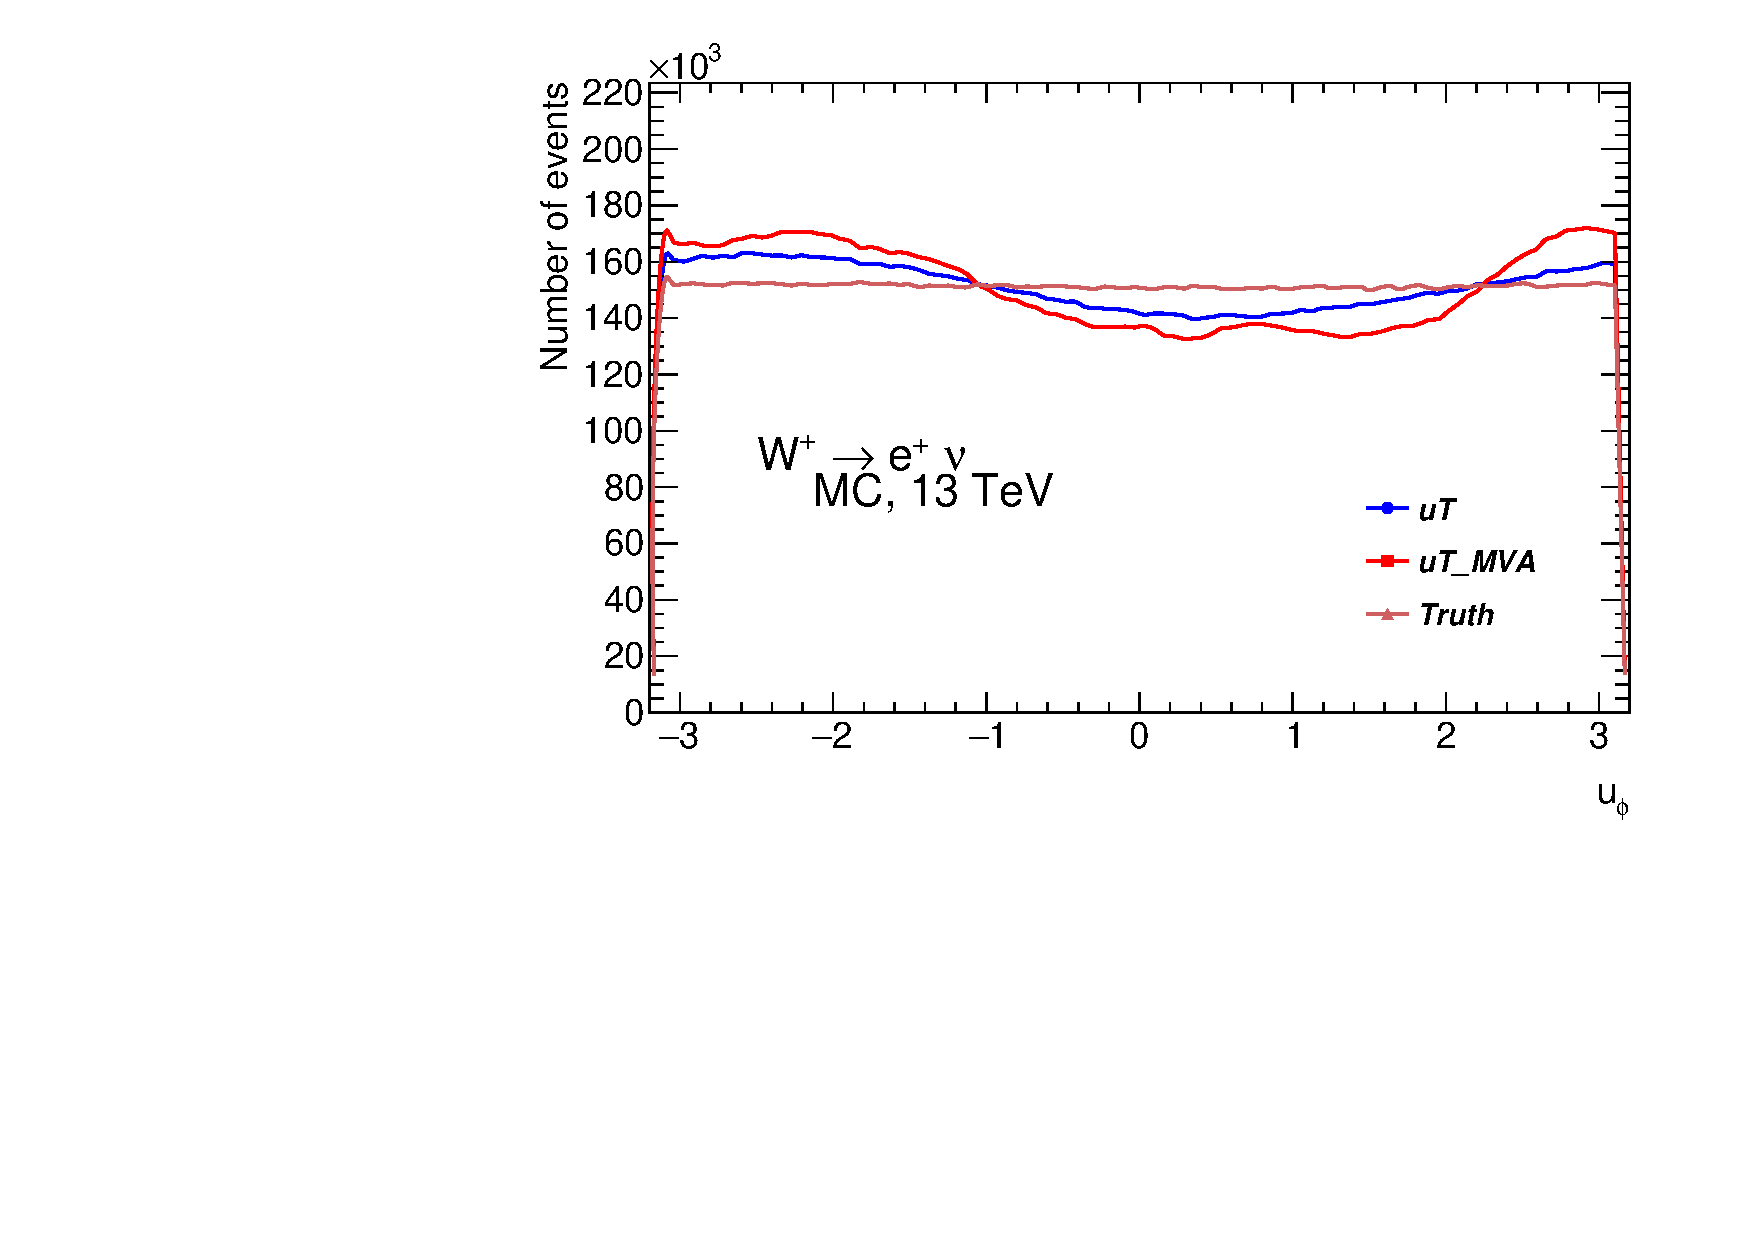
\includegraphics[width=.49\textwidth]{hist_uPhiplusenu.pdf}}\\
    	{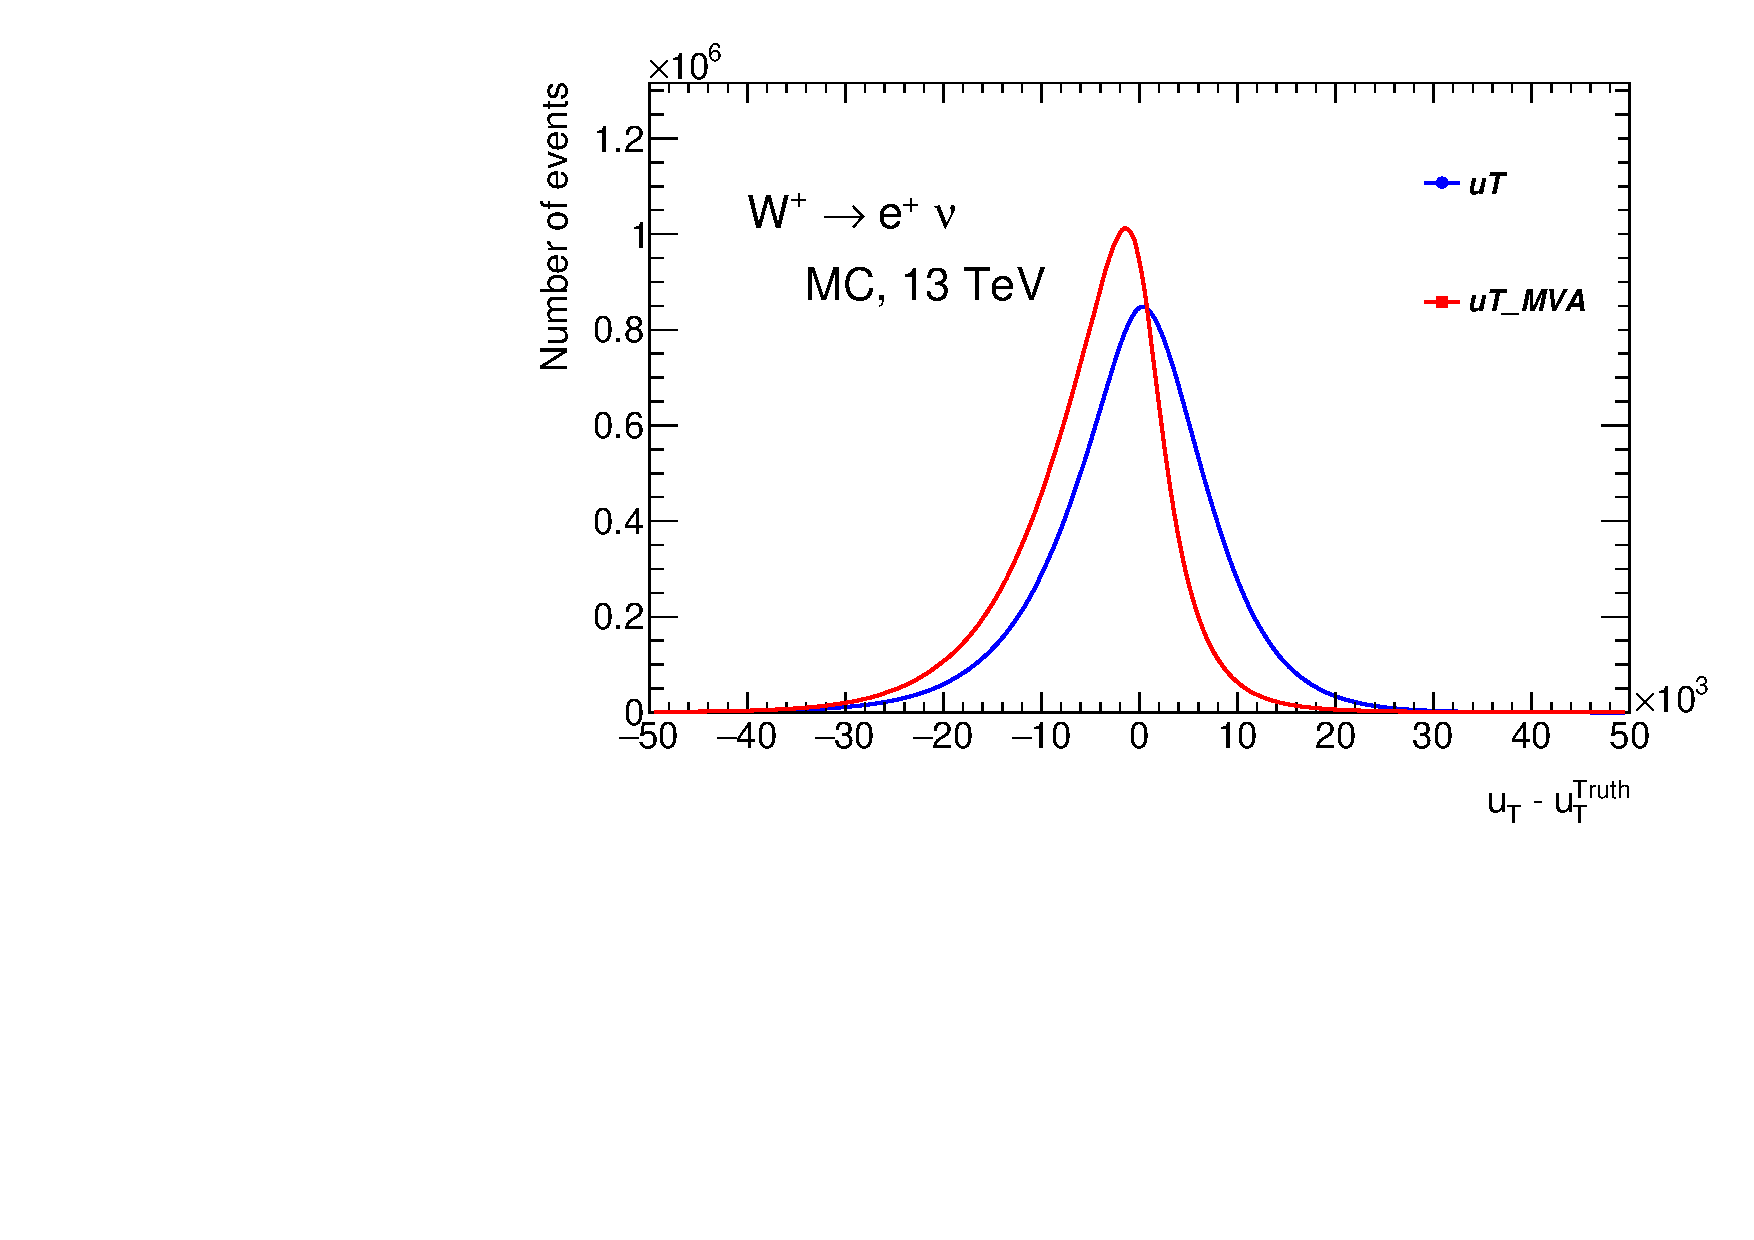
\includegraphics[width=.49\textwidth]{histosDeltaUtplusenu.pdf}}
    	{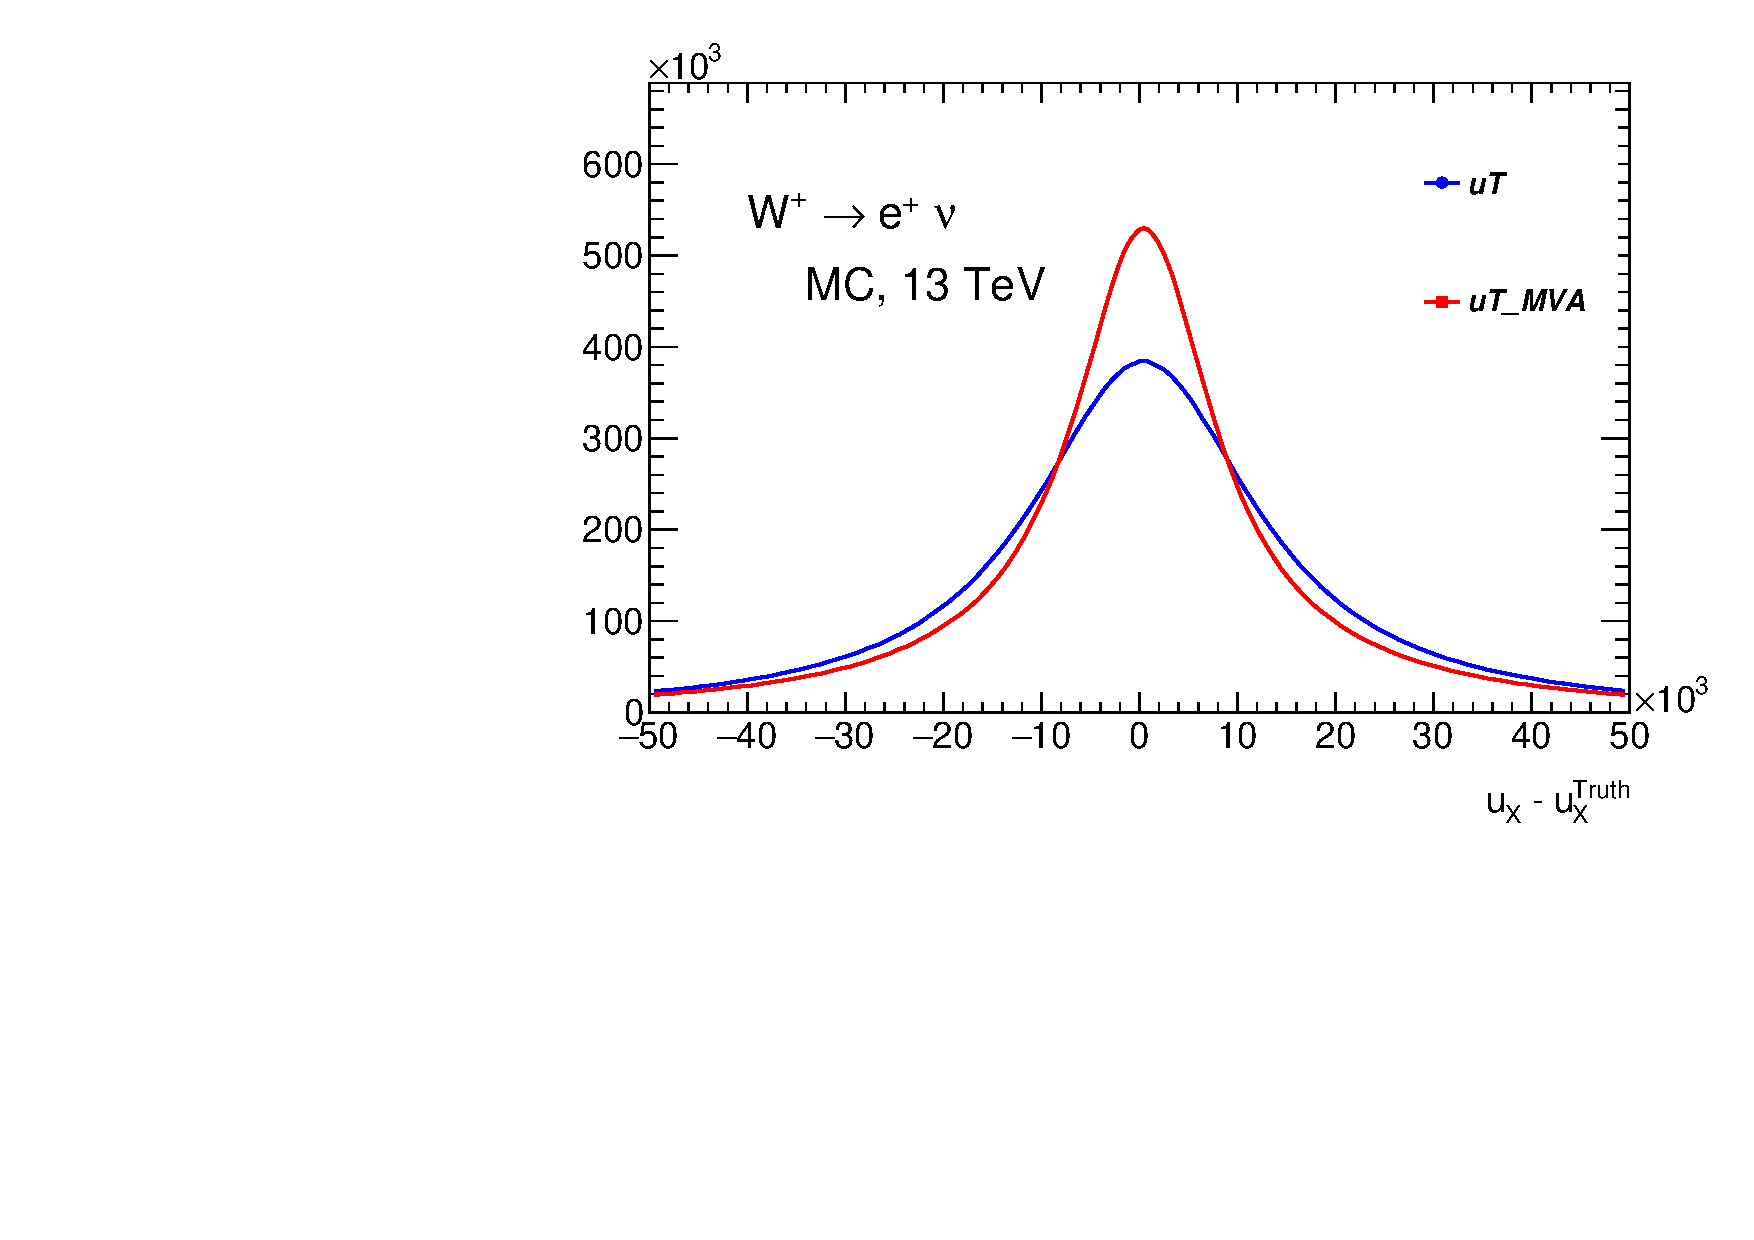
\includegraphics[width=.49\textwidth]{histosDeltaUxplusenu.pdf}} \\
    	{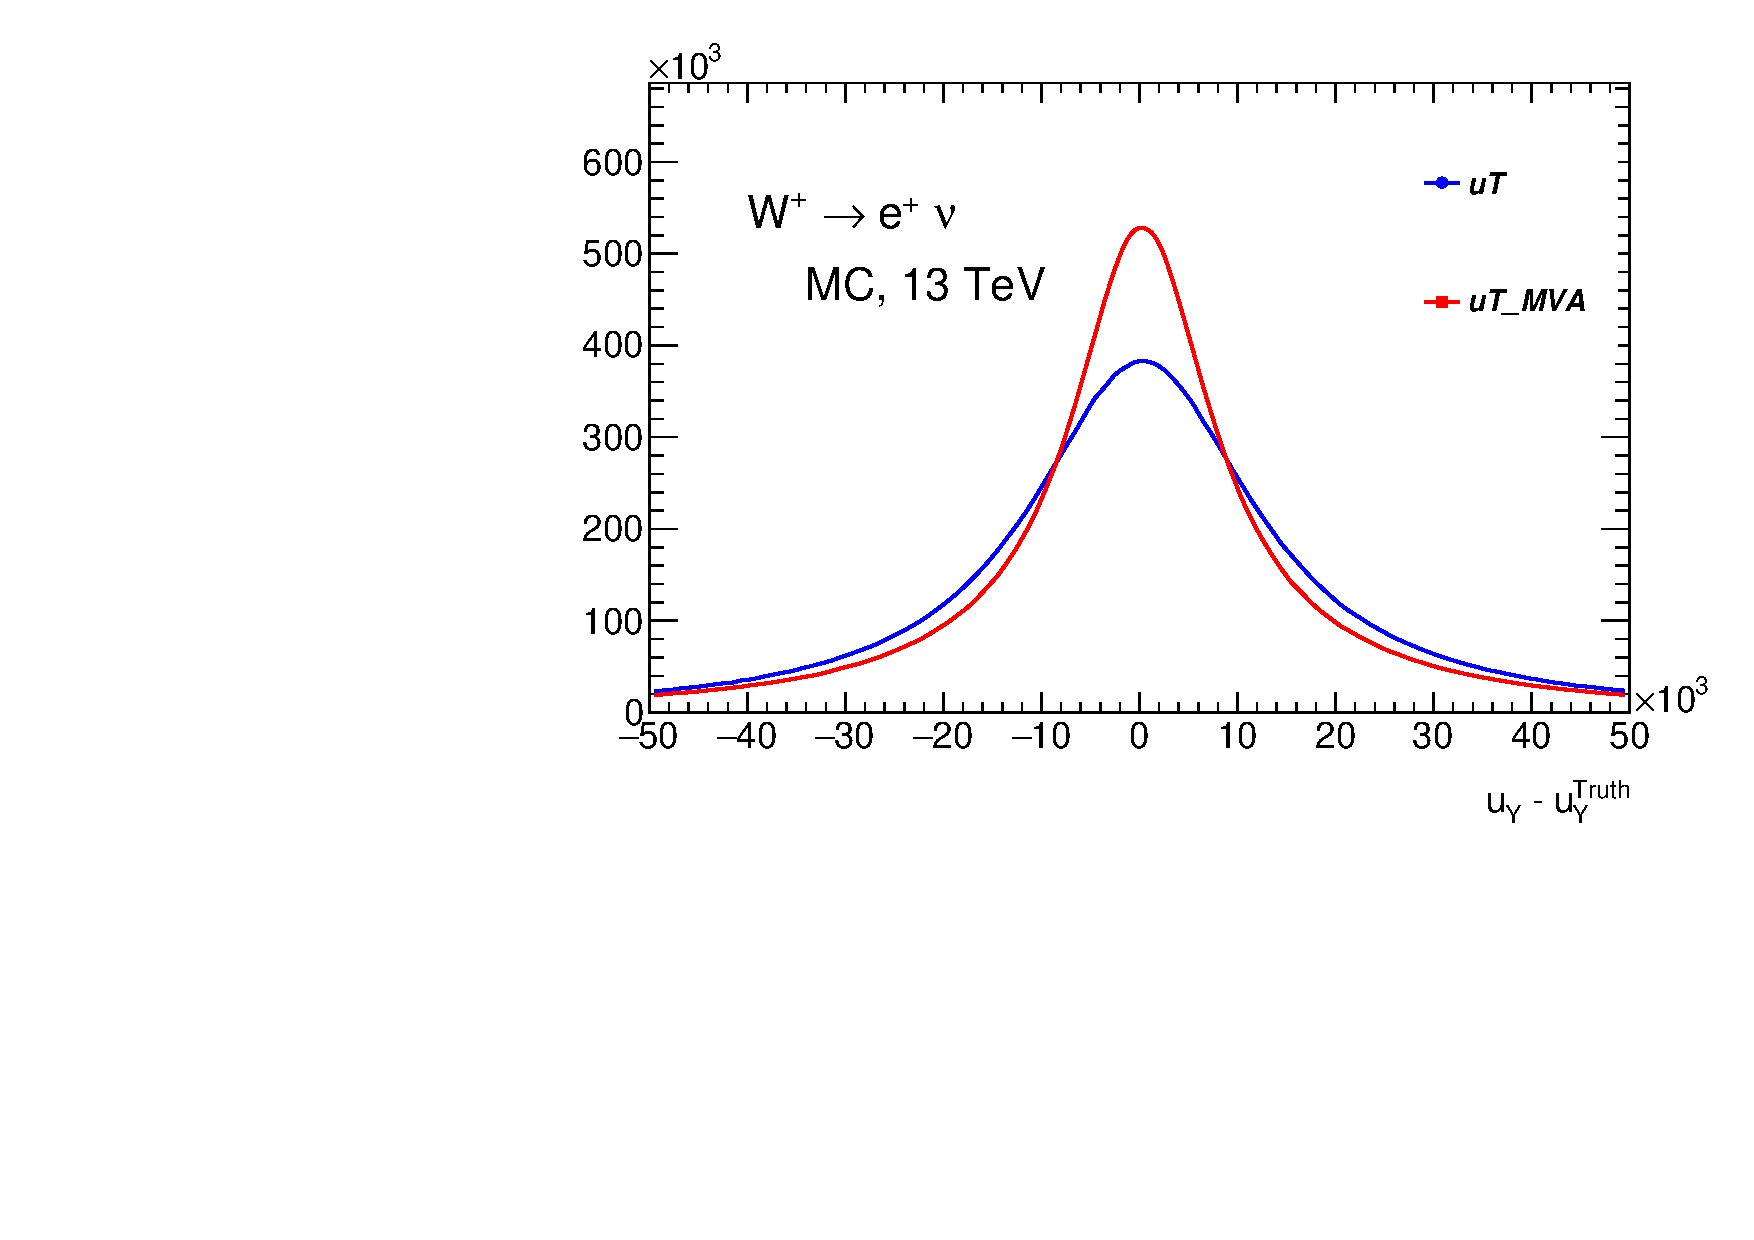
\includegraphics[width=.49\textwidth]{histosDeltaUyplusenu.pdf}}
    	{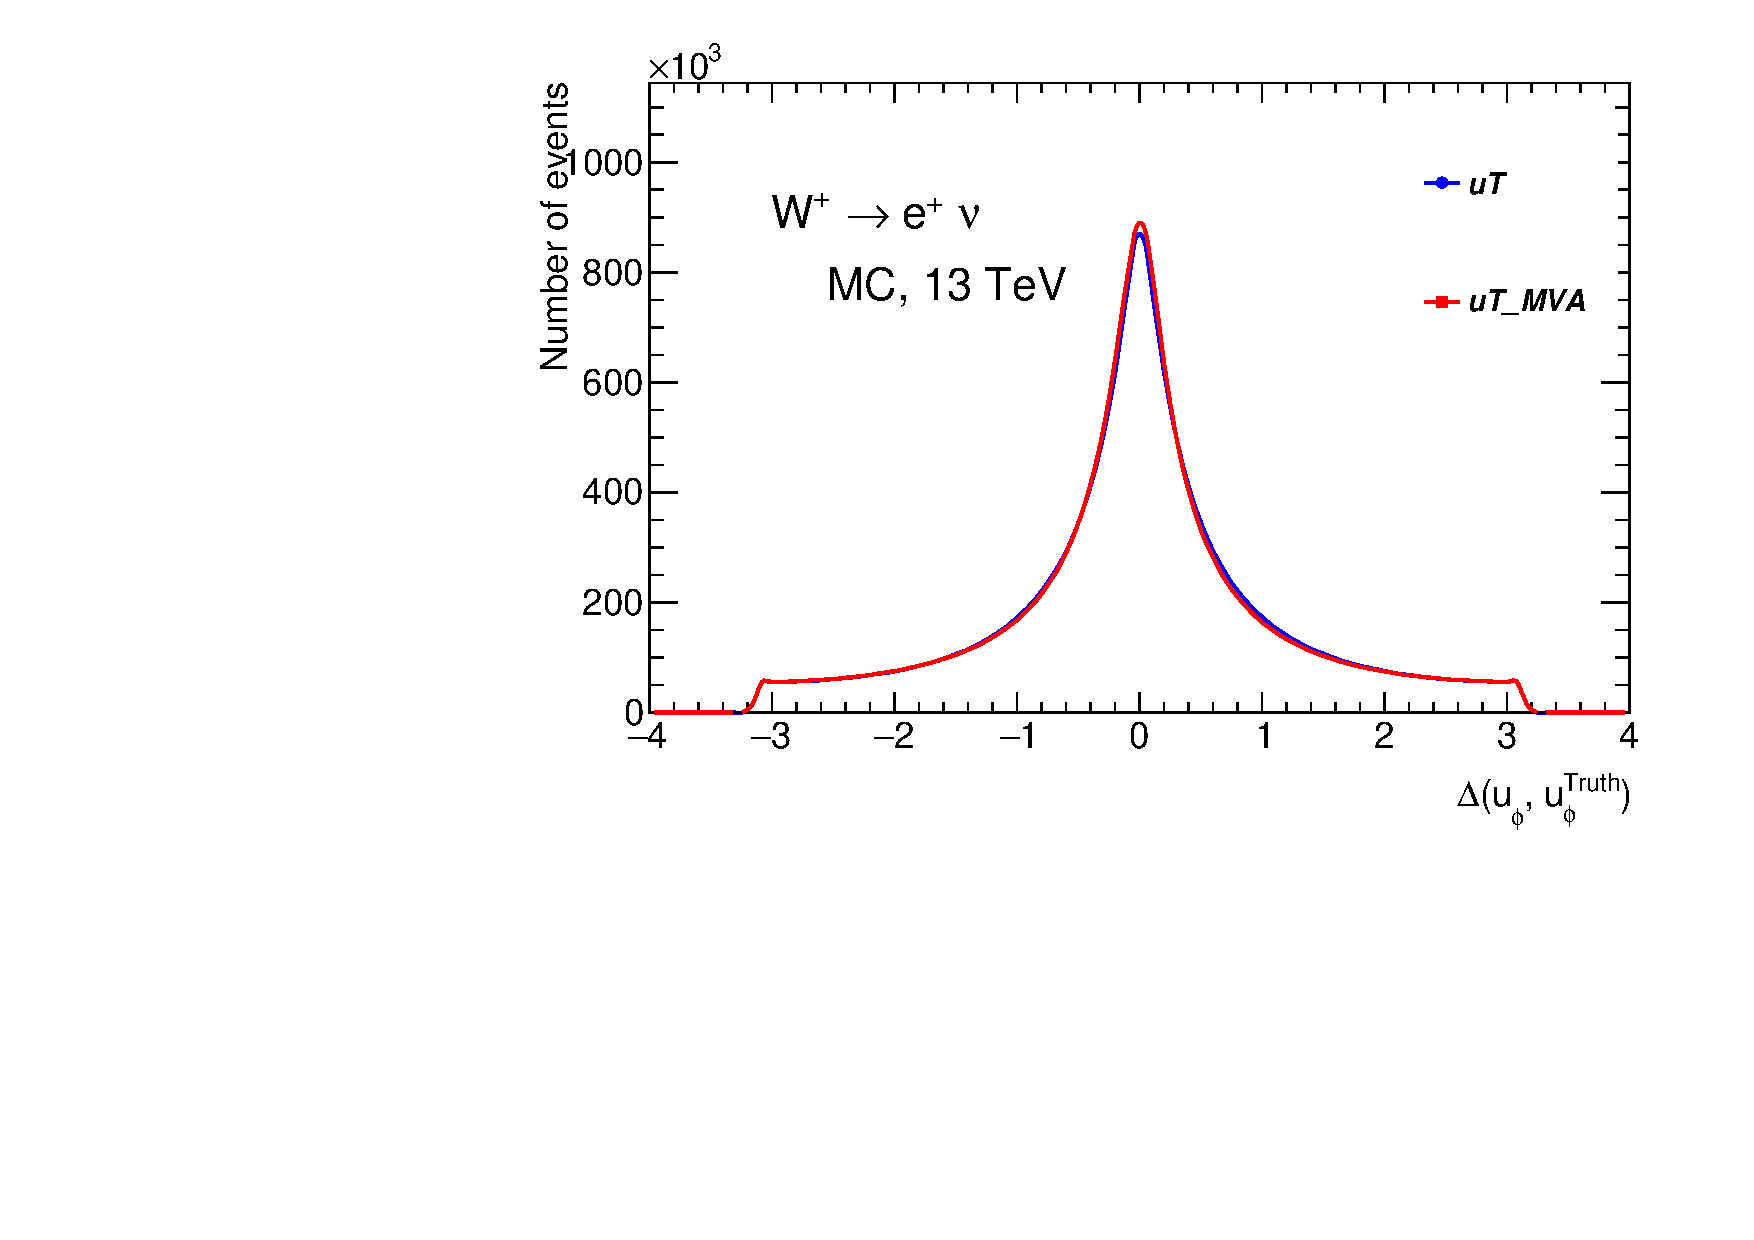
\includegraphics[width=.49\textwidth]{histosDeltaUPhiplusenu.pdf}}\\
    	\label{fig:plusenu_data_distributions1}
    \end{figure}
    \begin{figure}[h]
    	\centering
    	{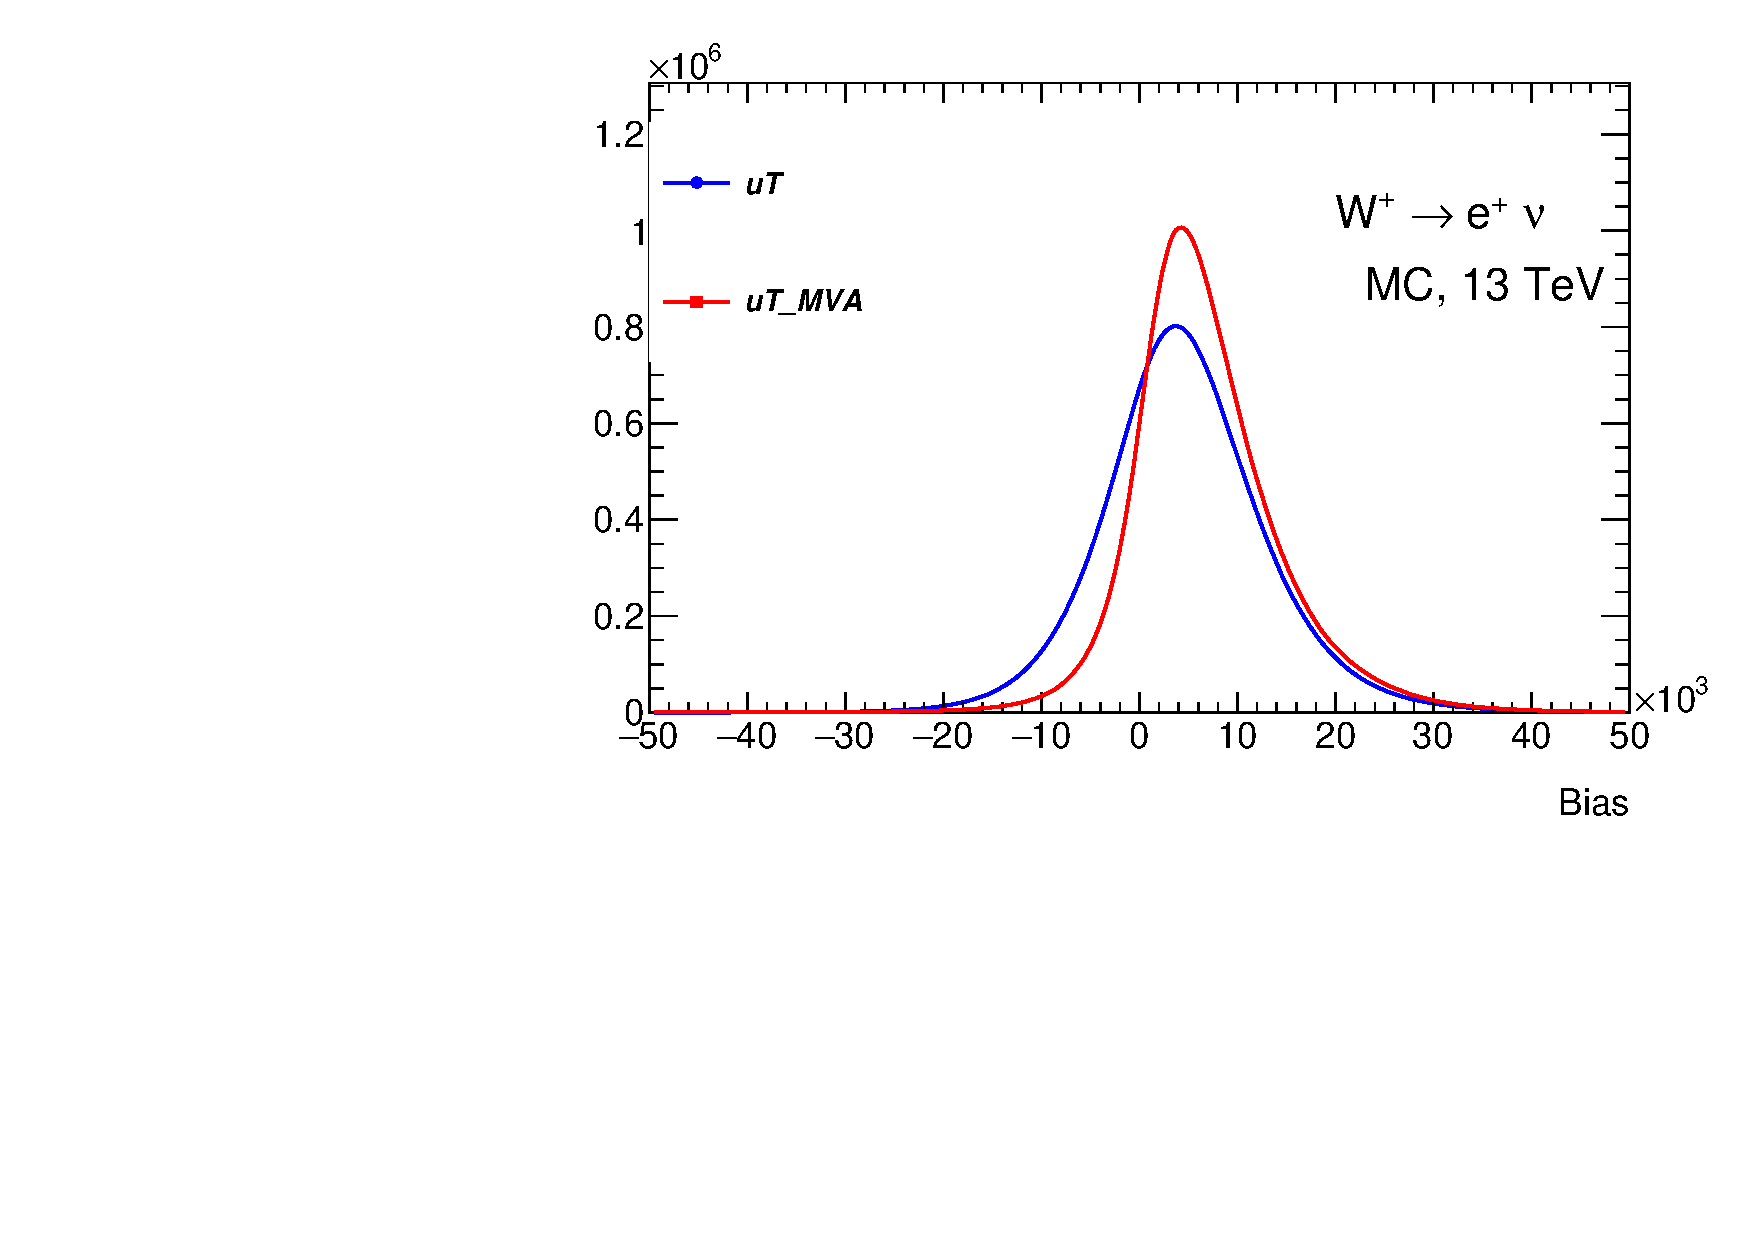
\includegraphics[width=.49\textwidth]{outMVA_biasplusenu}}
    	{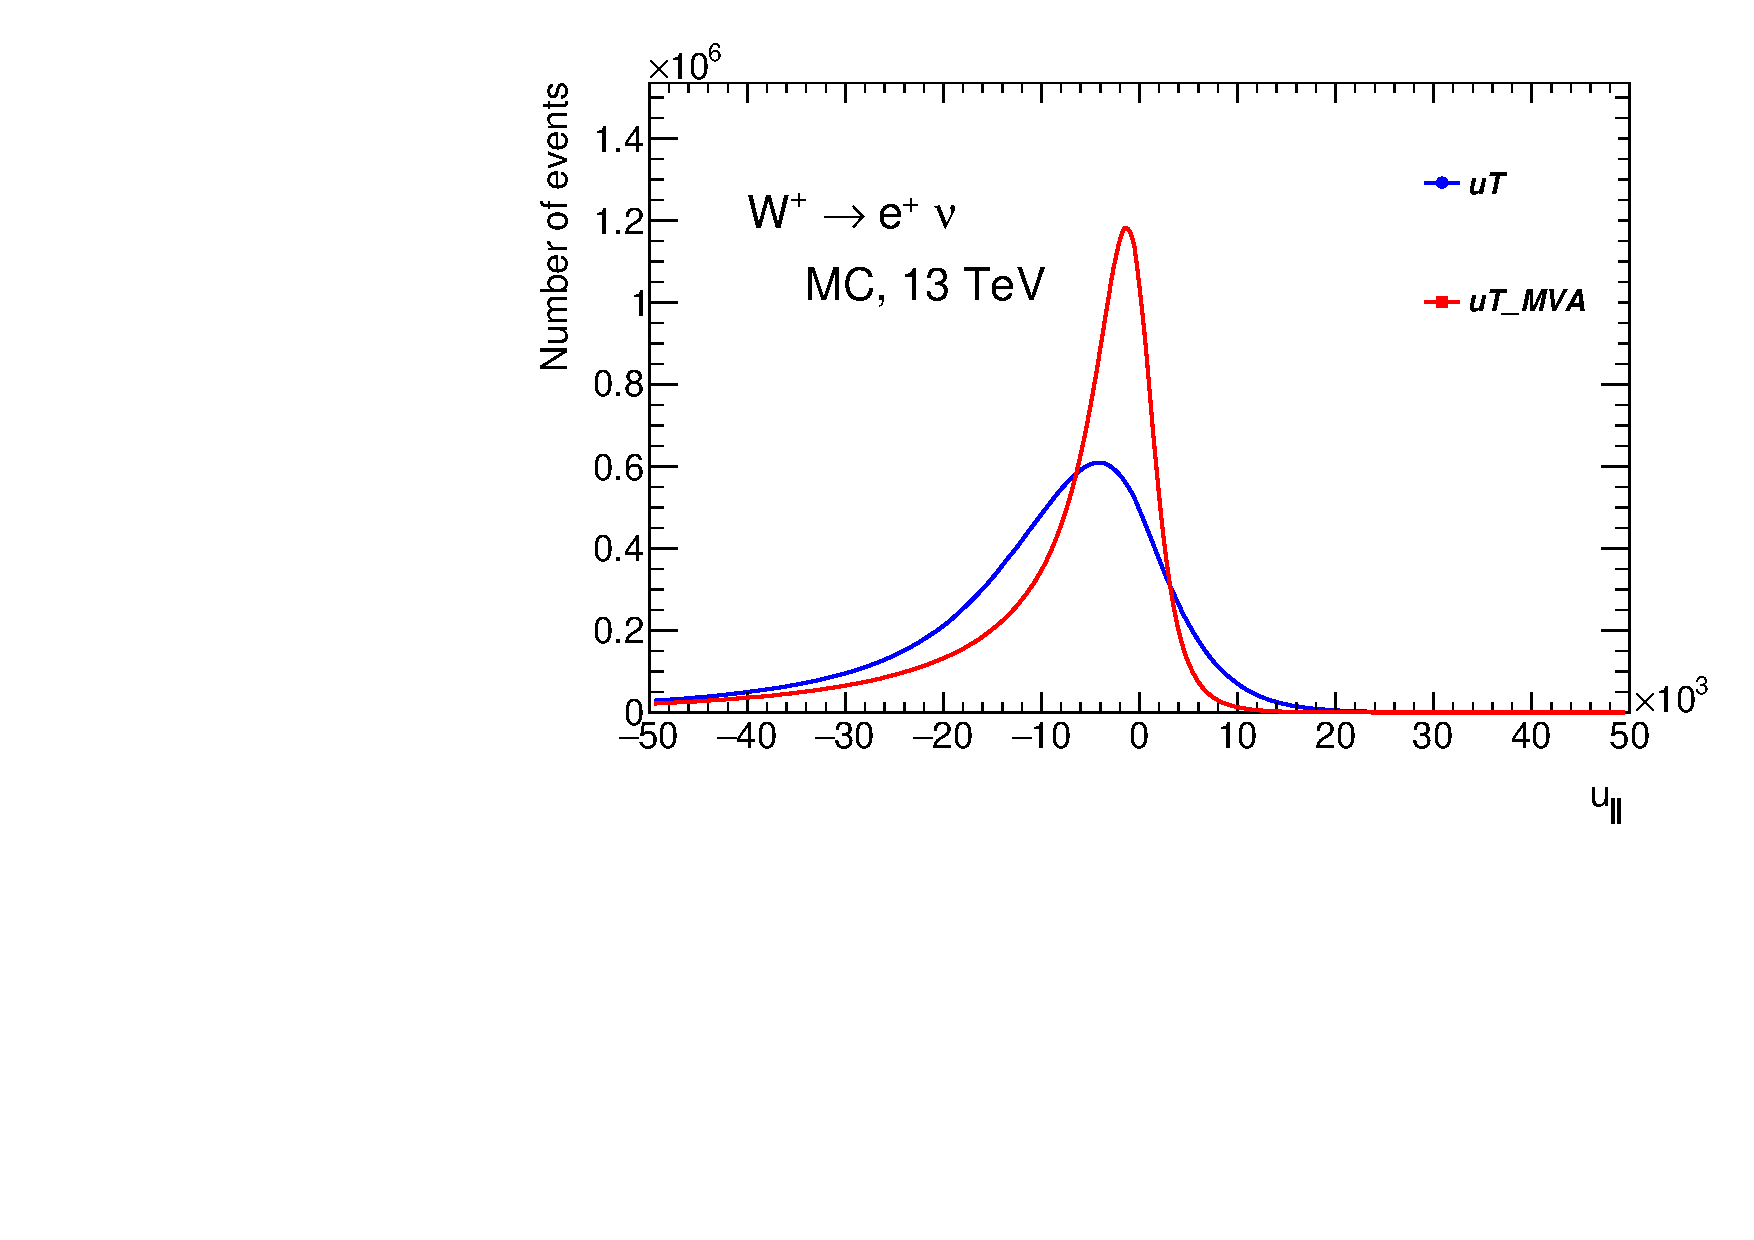
\includegraphics[width=.49\textwidth]{outMVA_Uparplusenu}}
    	{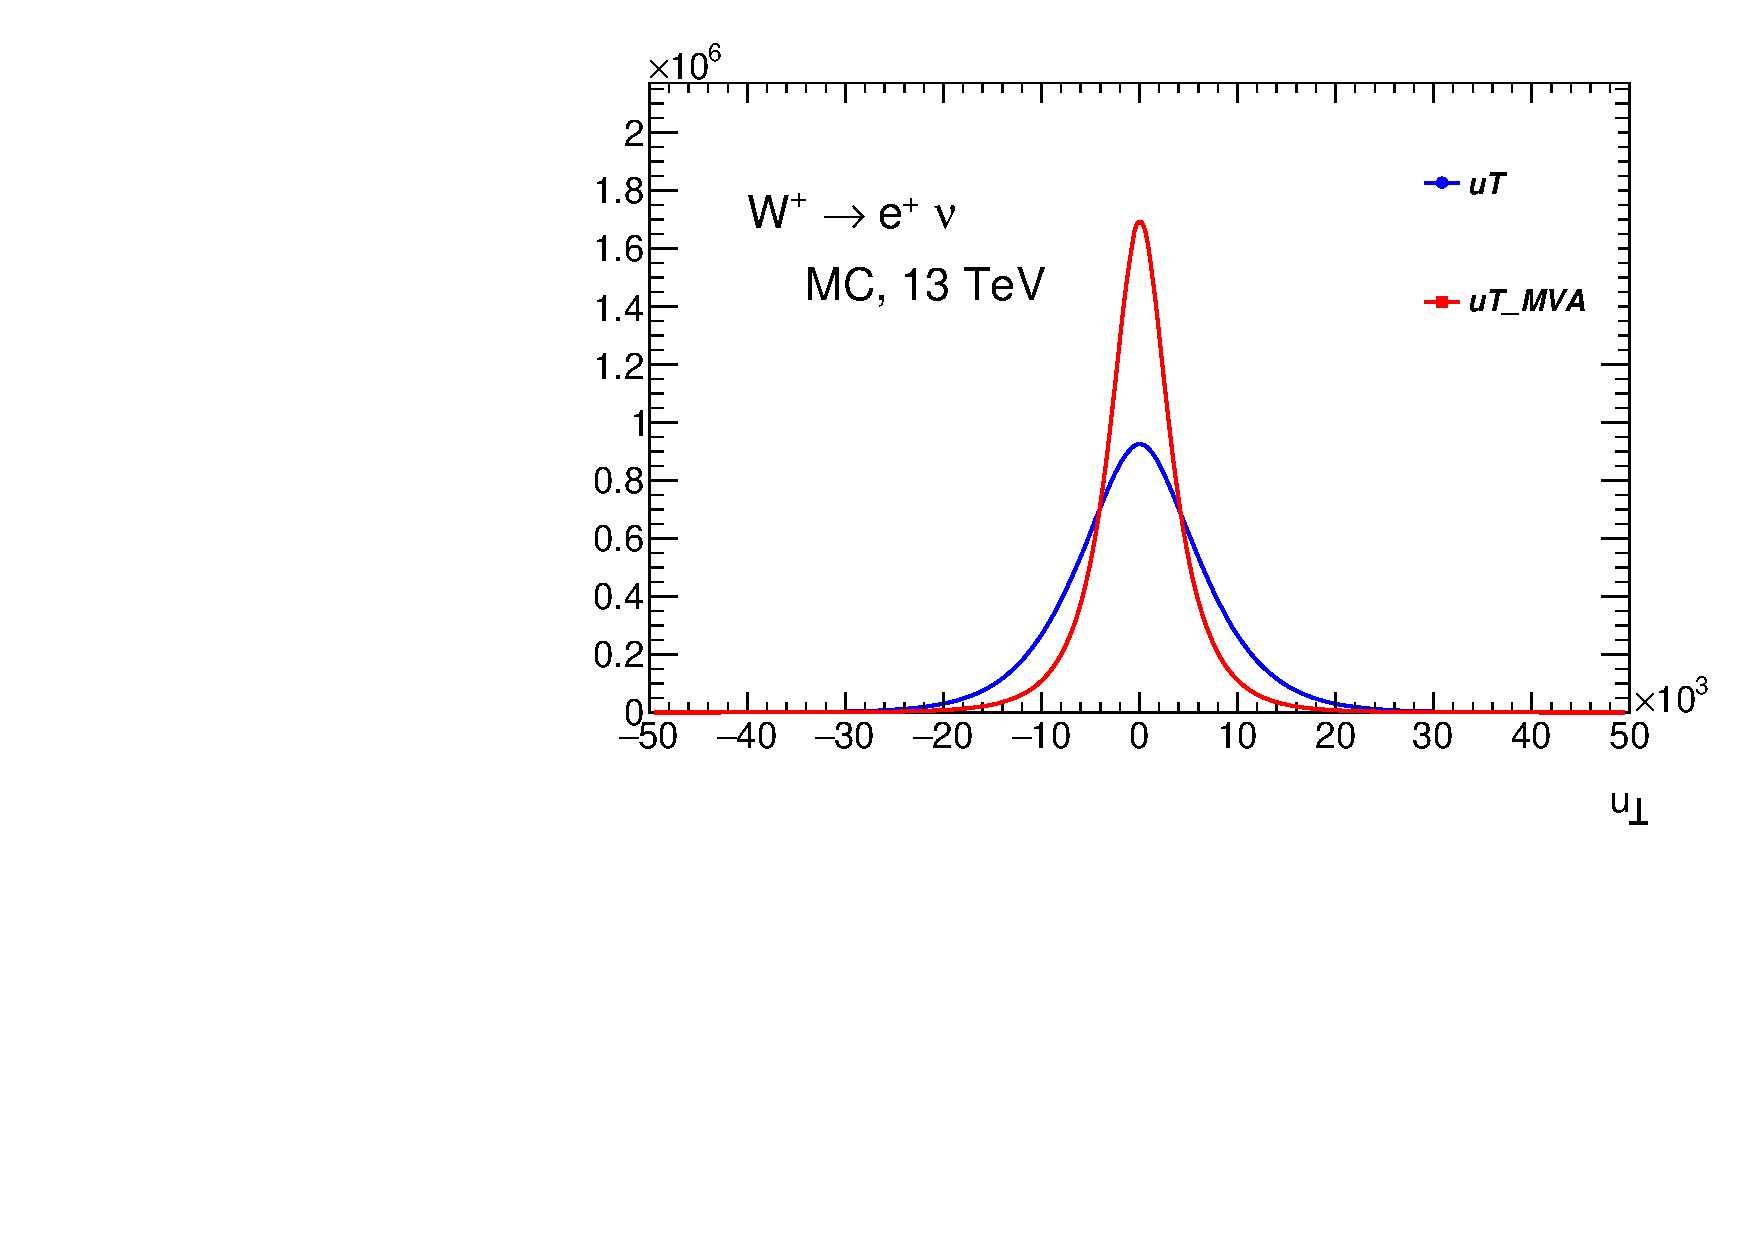
\includegraphics[width=.49\textwidth]{outMVA_uPerpplusenu}}
    	{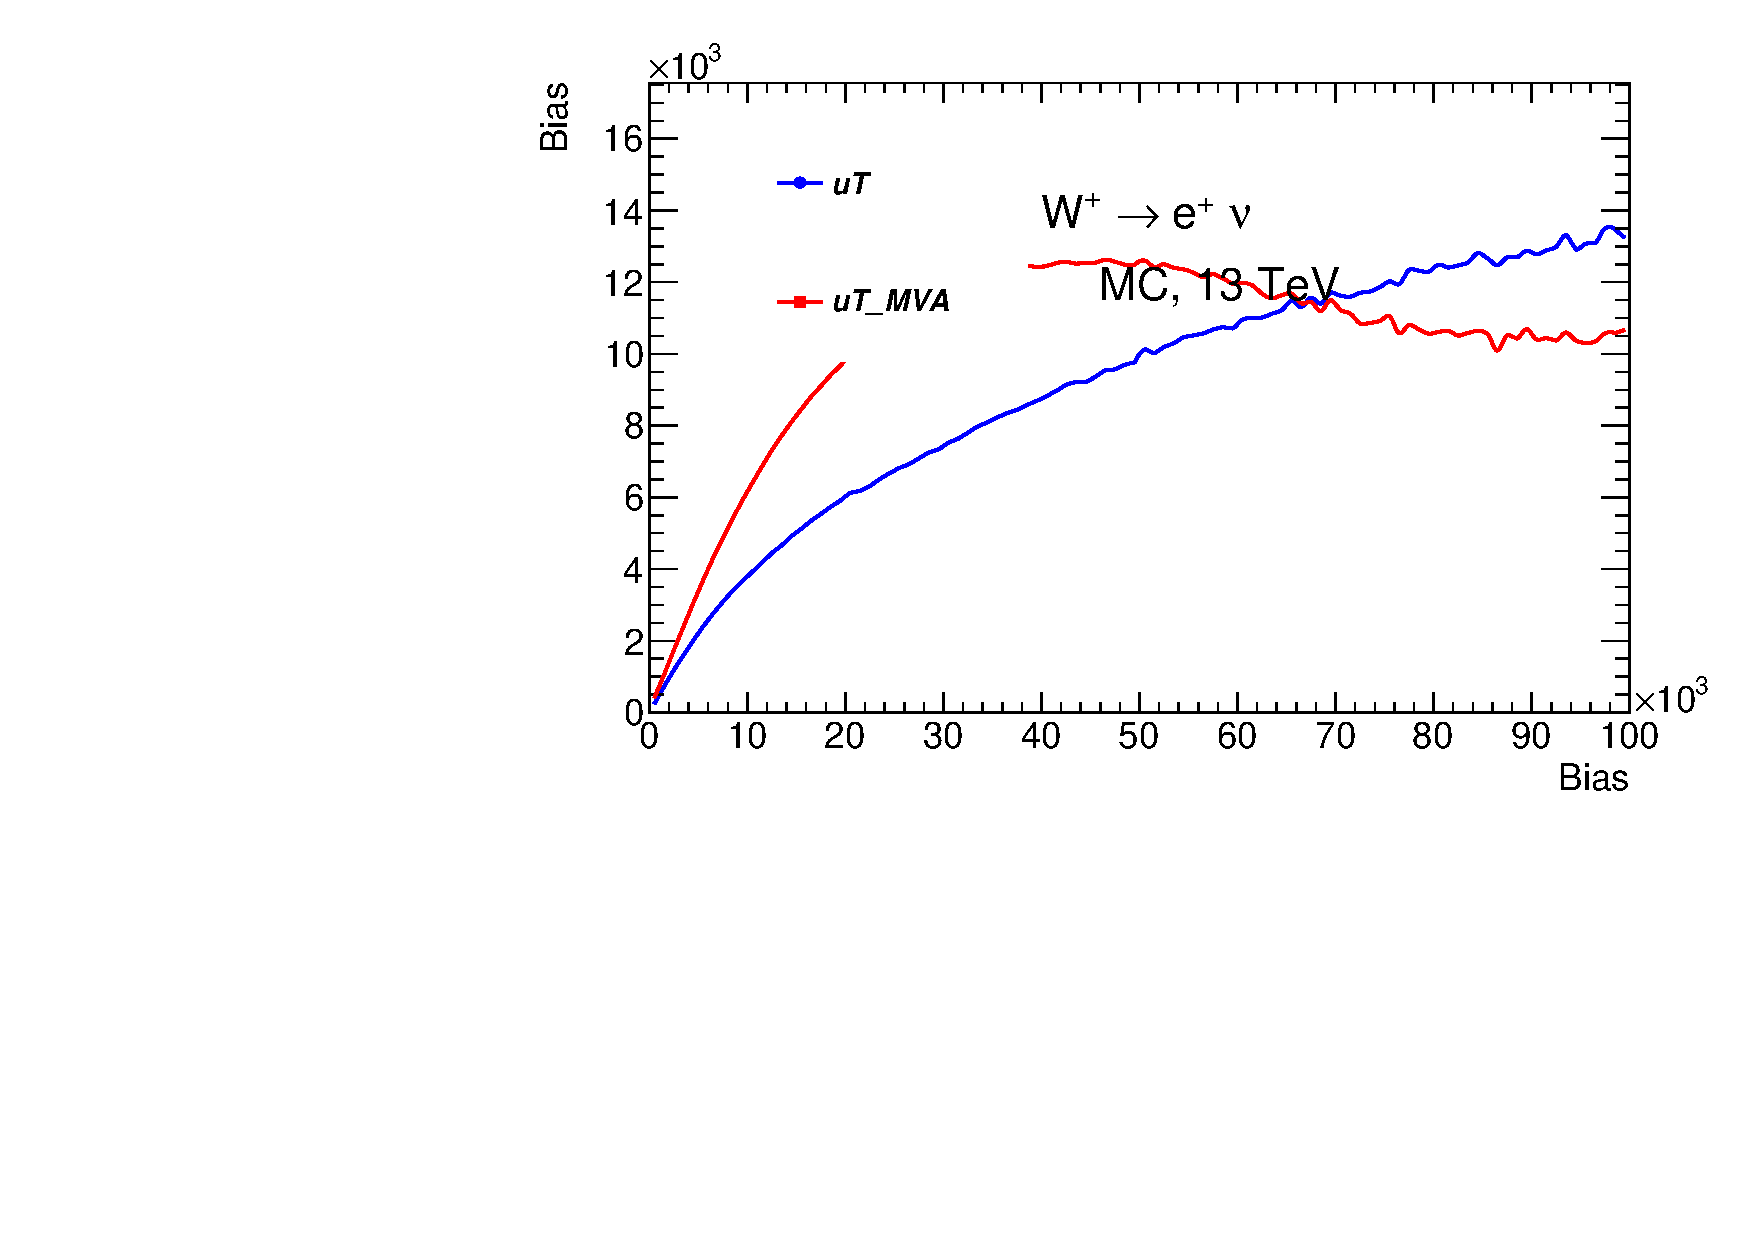
\includegraphics[width=.49\textwidth]{histosMeanBiasplusenu}}
    	{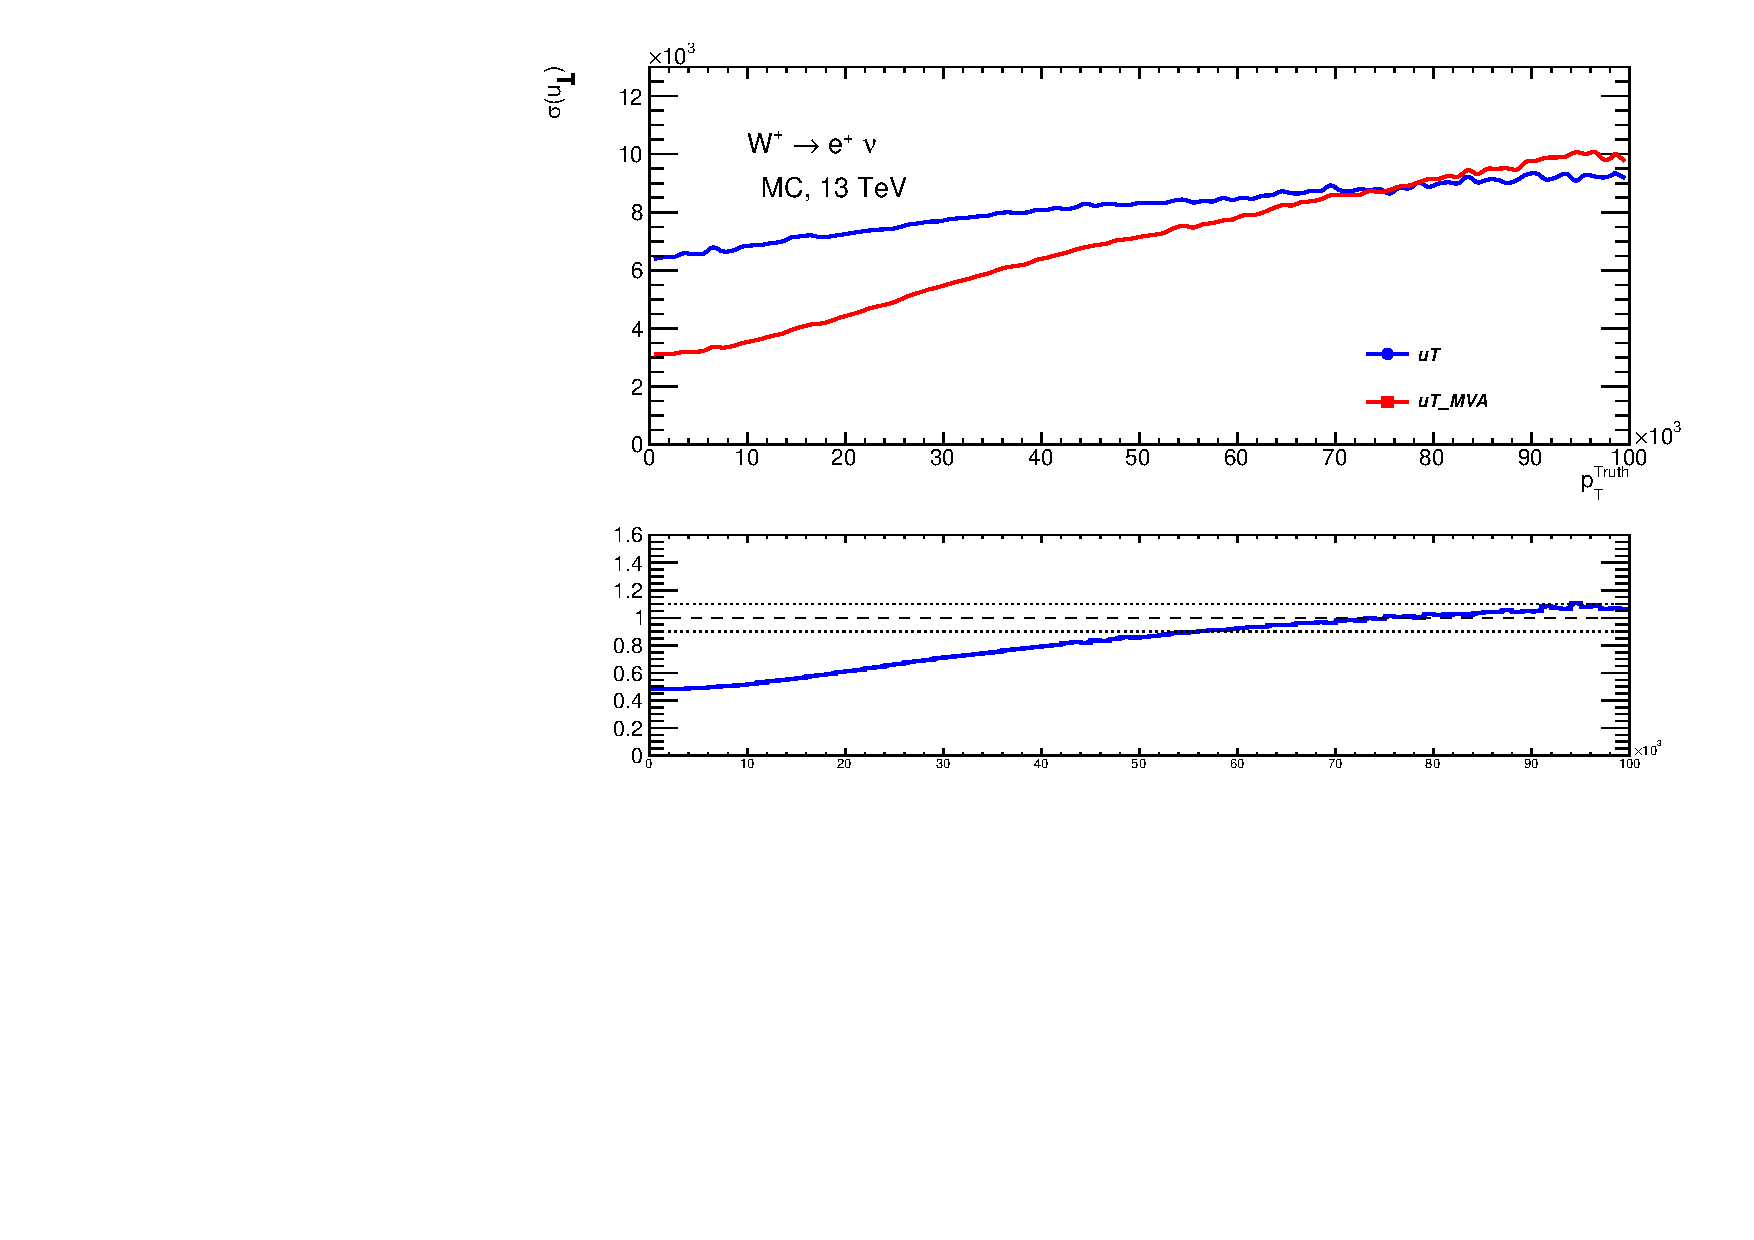
\includegraphics[width=.49\textwidth]{histosSigmaUperpplusenu}}
    	{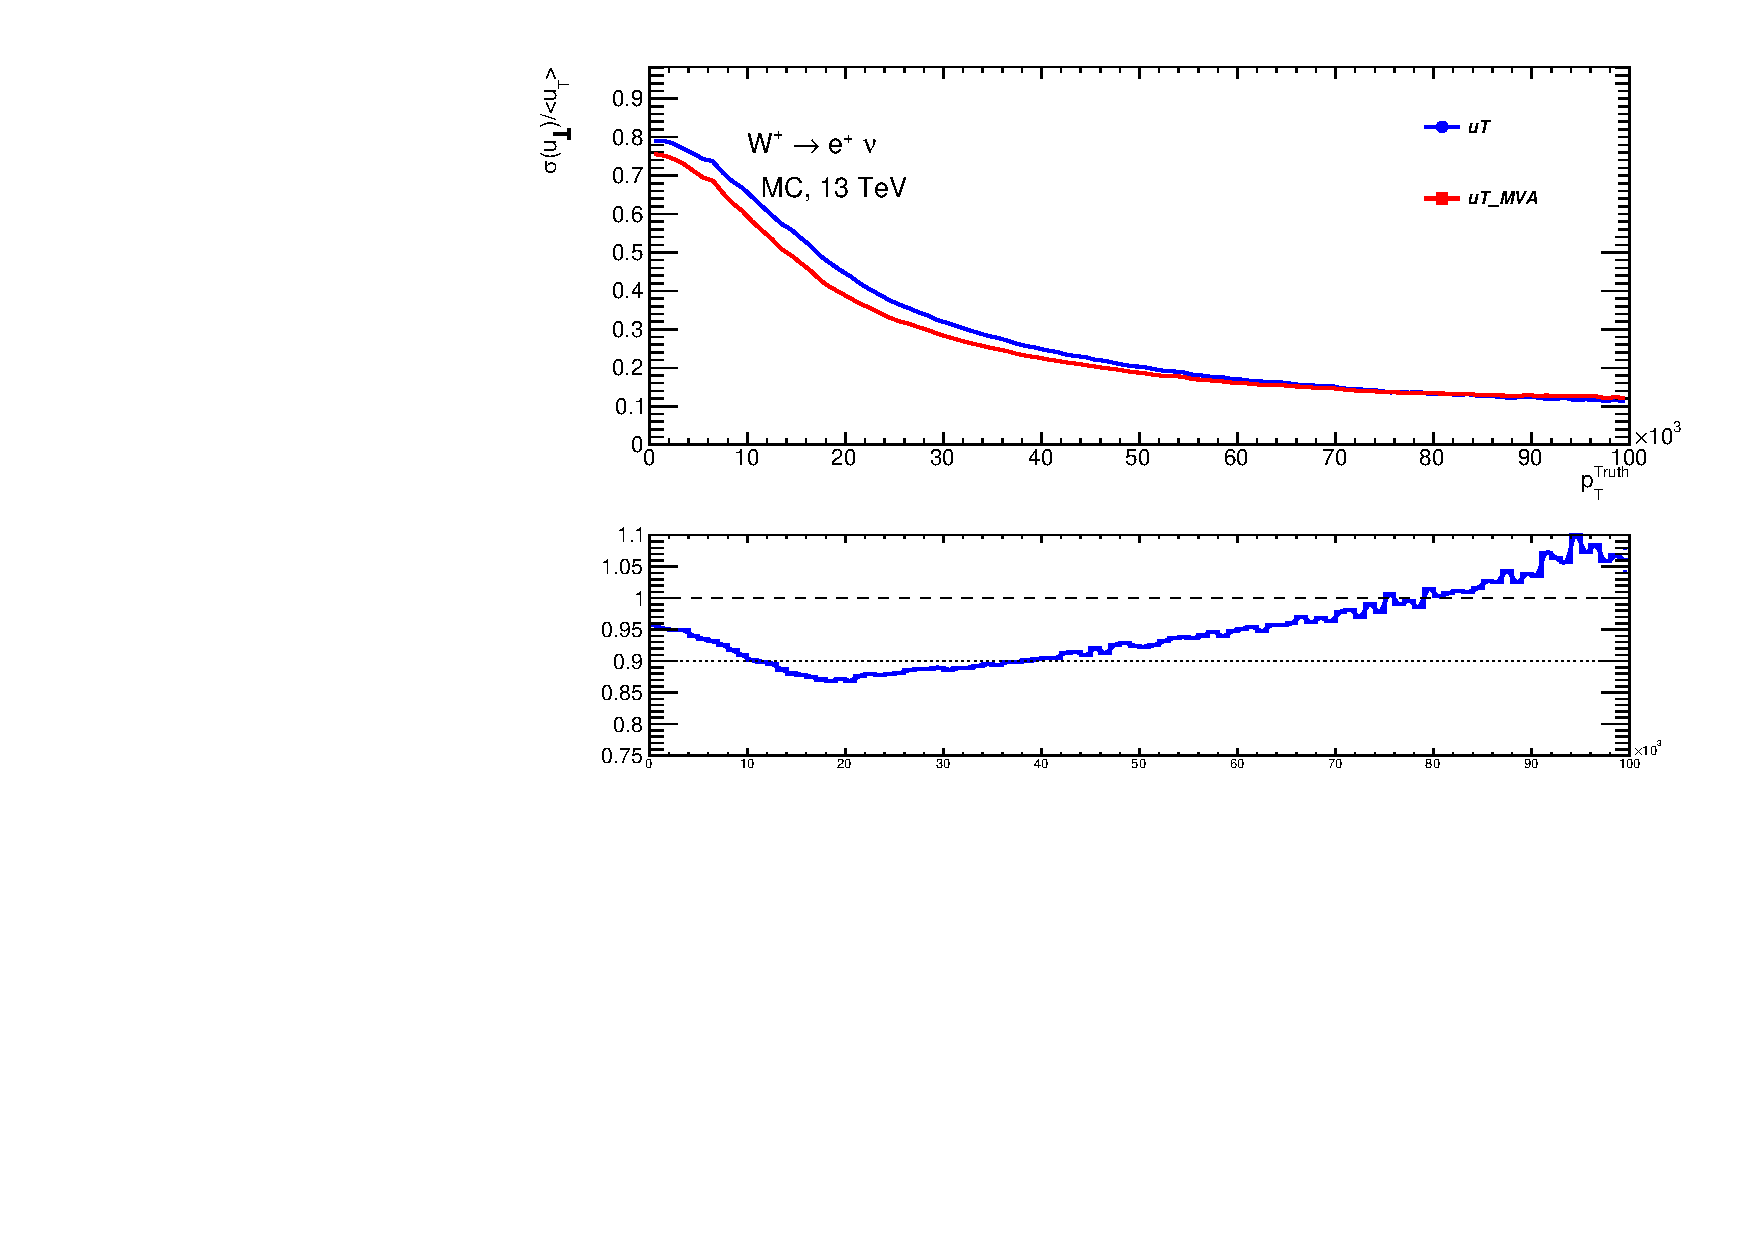
\includegraphics[width=.49\textwidth]{histosUperpRelativeplusenu}}
    	\caption{Comparison of kinematic distributions of $u_T$ vs $u_T^{MVA}$ for $W^+\rightarrow e^+\nu$ data sample.}
    	\label{fig:plusenu_data_distributions2}
    \end{figure}
    
        \begin{figure}[h]
    	\centering
    	{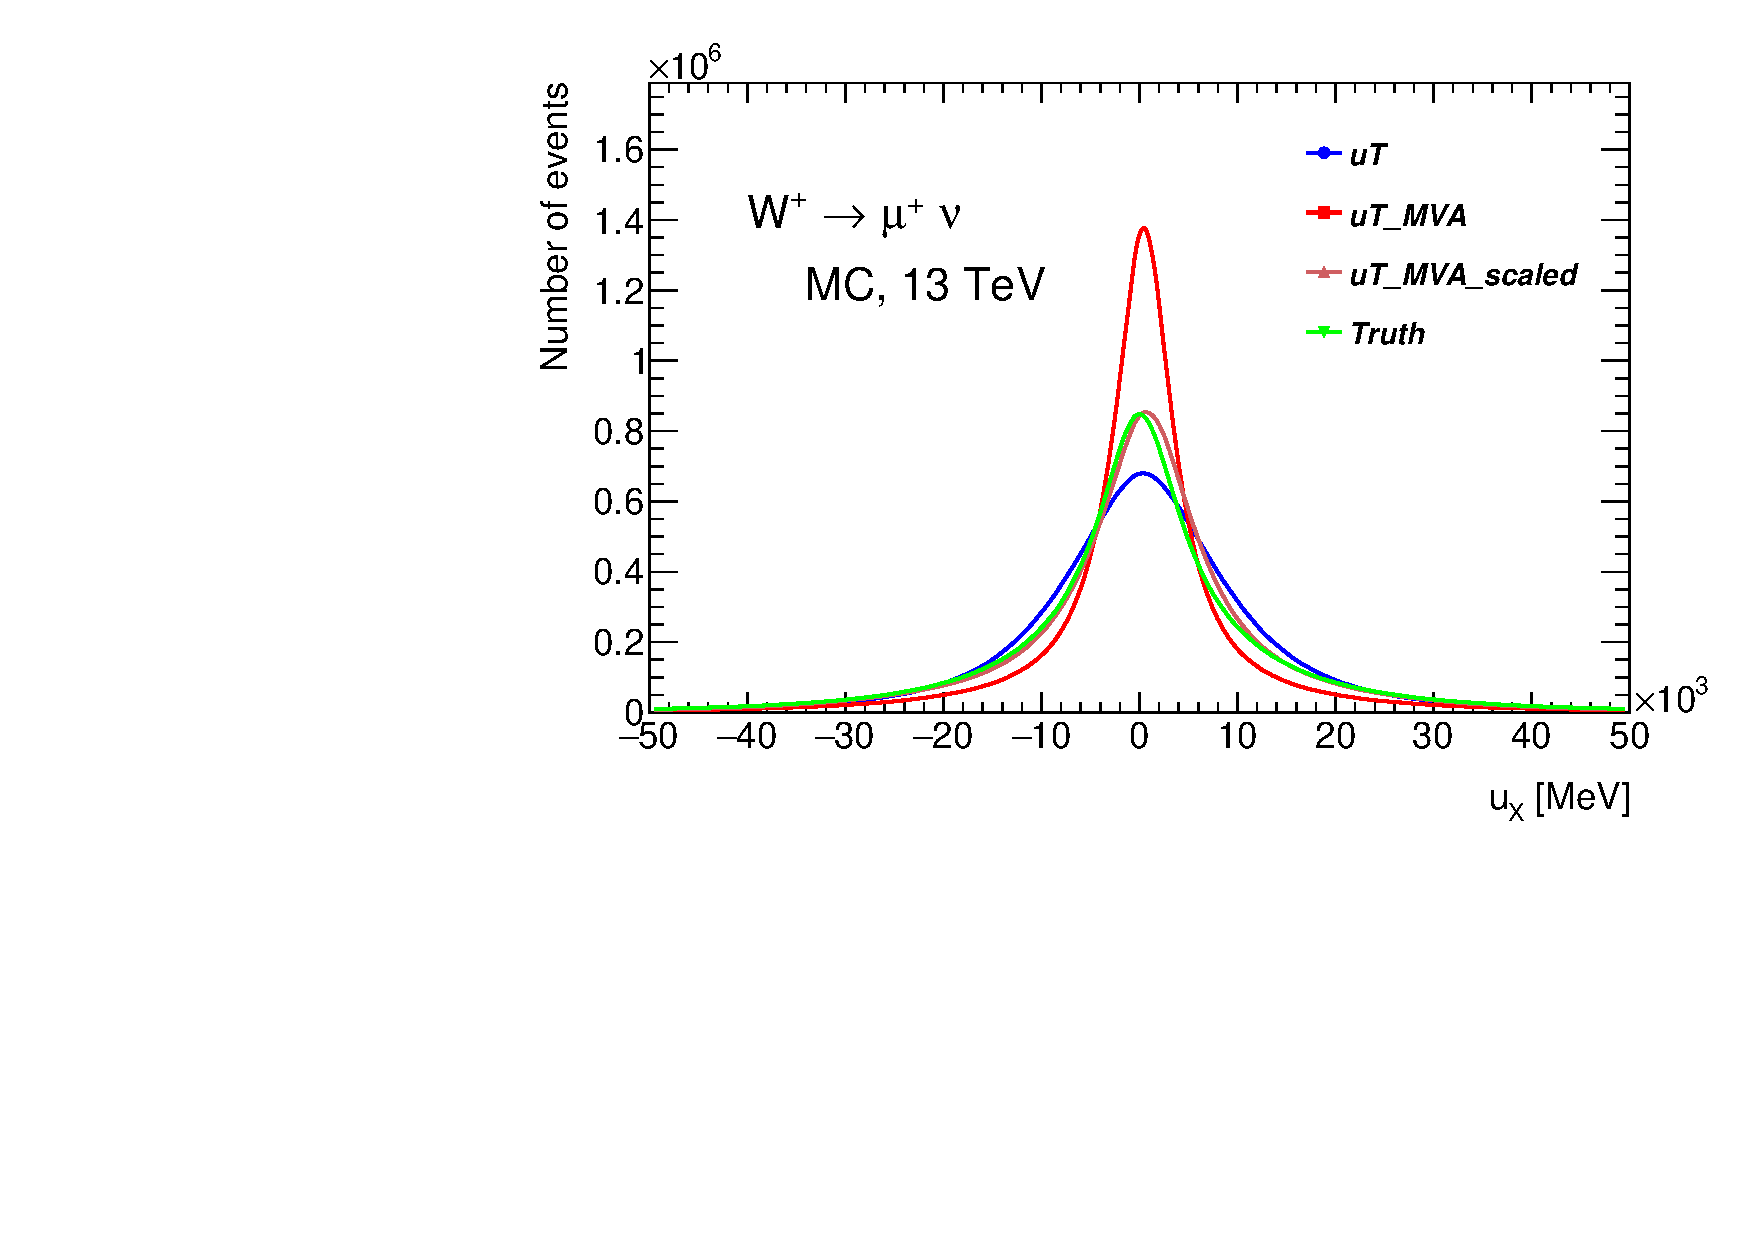
\includegraphics[width=.49\textwidth]{hist_uXplusmunu.pdf}}
    	{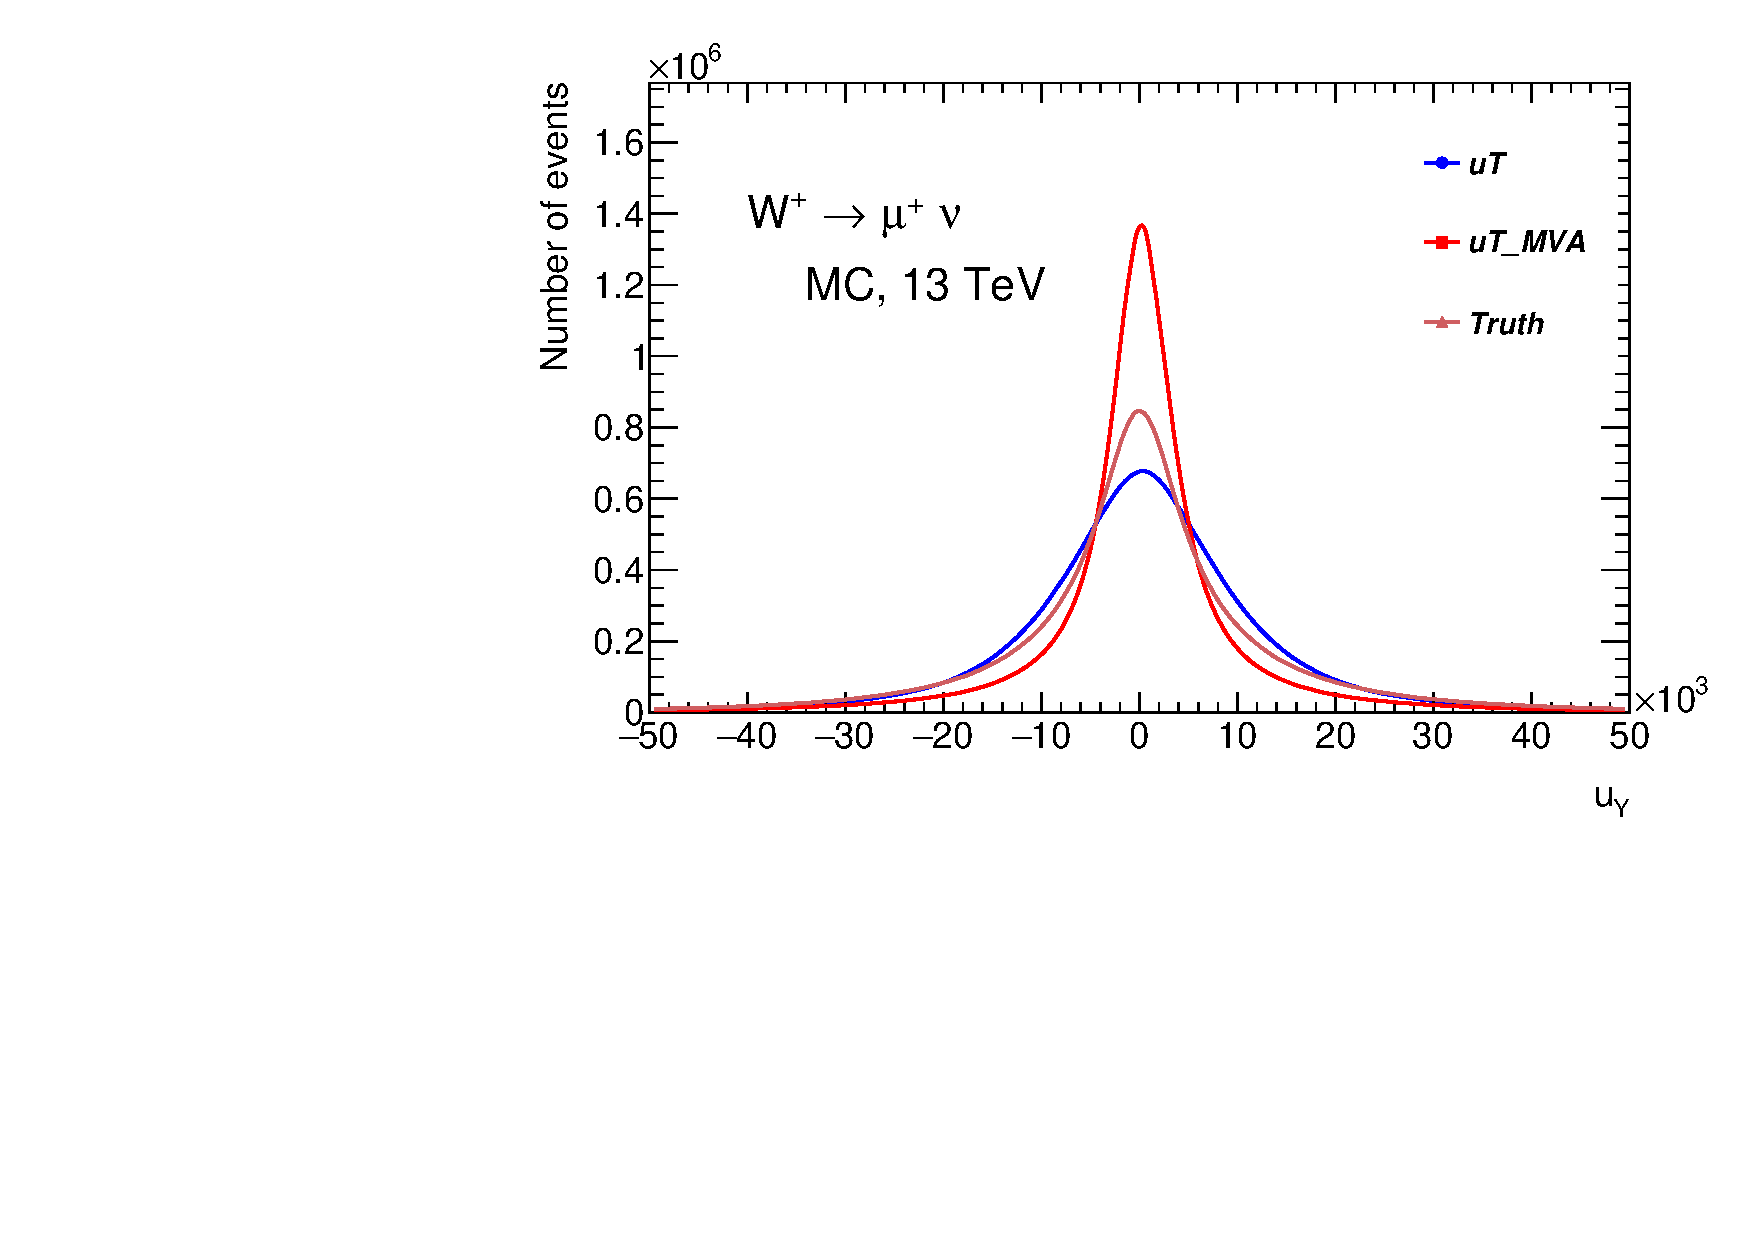
\includegraphics[width=.49\textwidth]{hist_uYplusmunu.pdf}} \\
    	{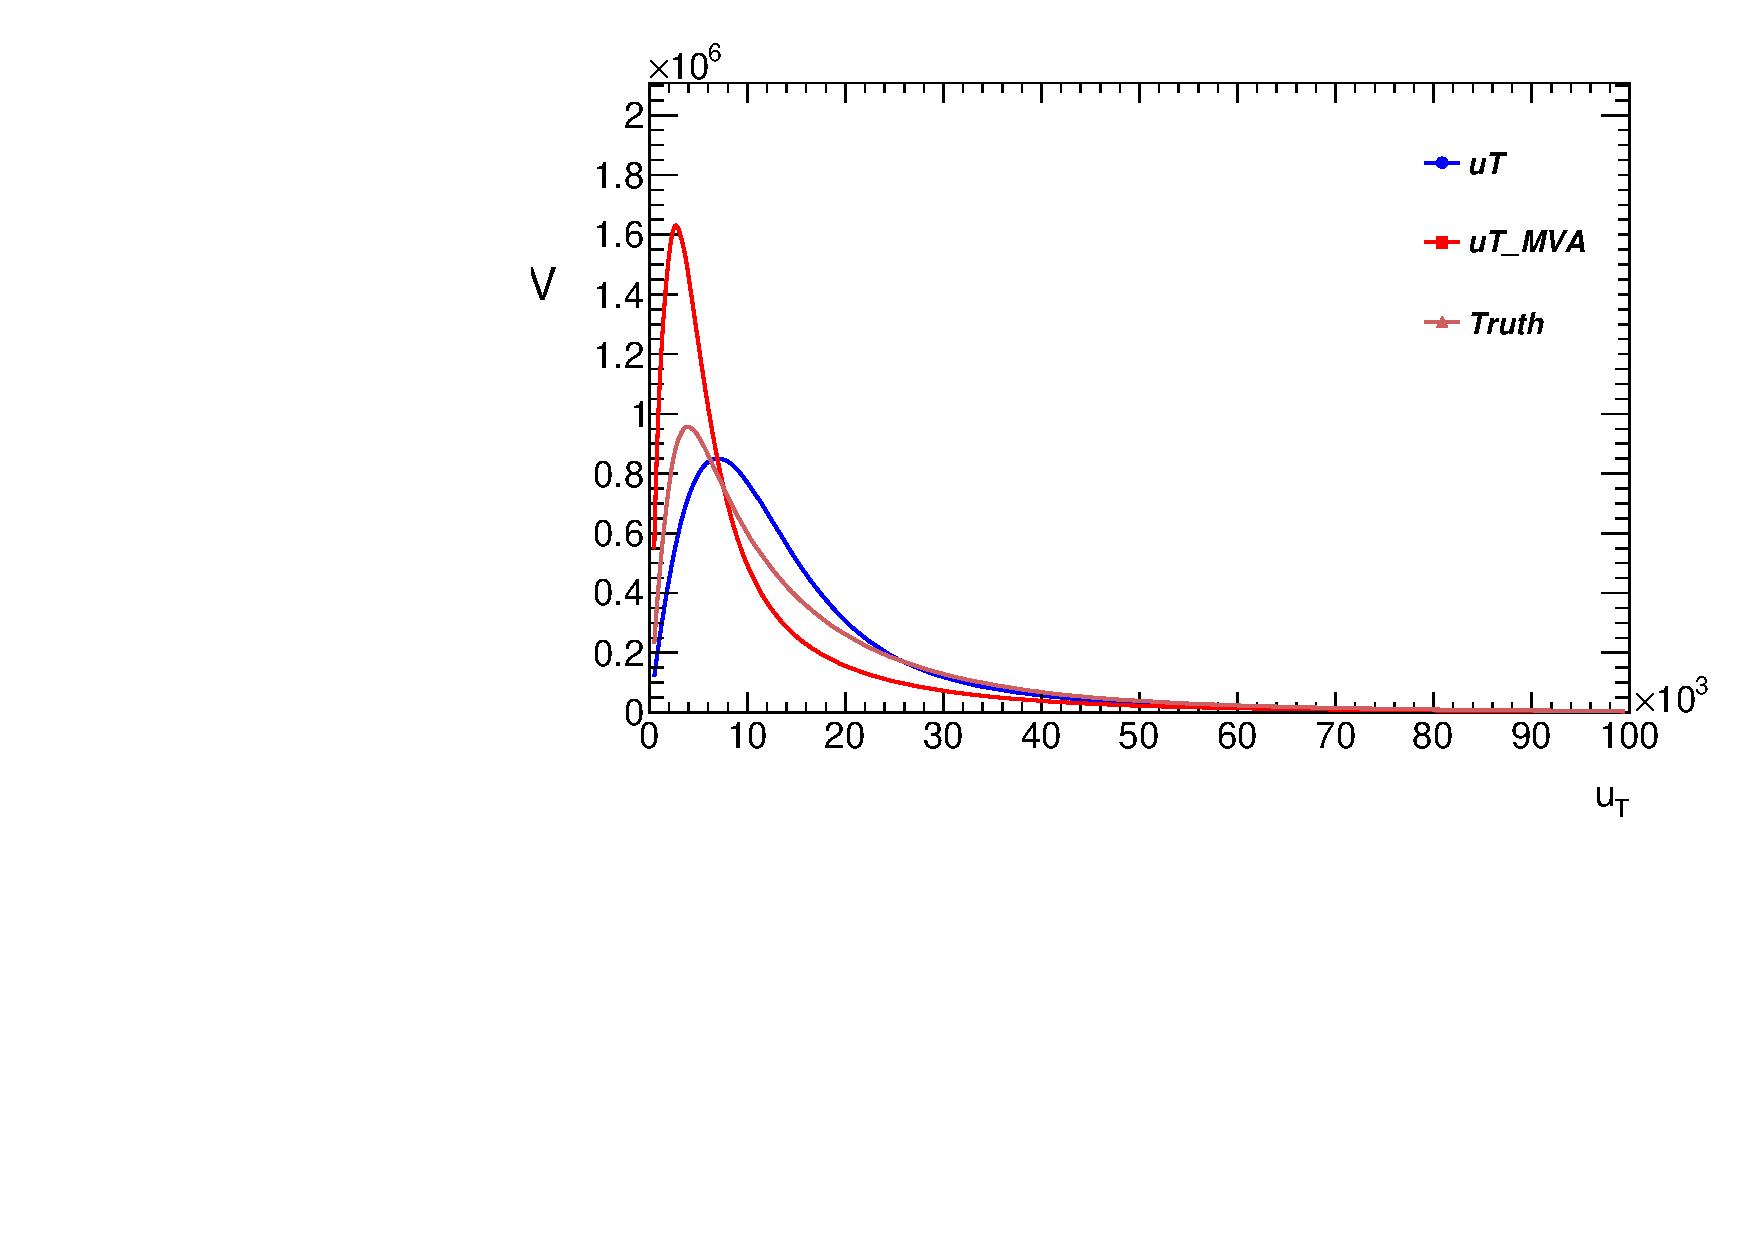
\includegraphics[width=.49\textwidth]{hist_uTplusmunu.pdf}}
    	{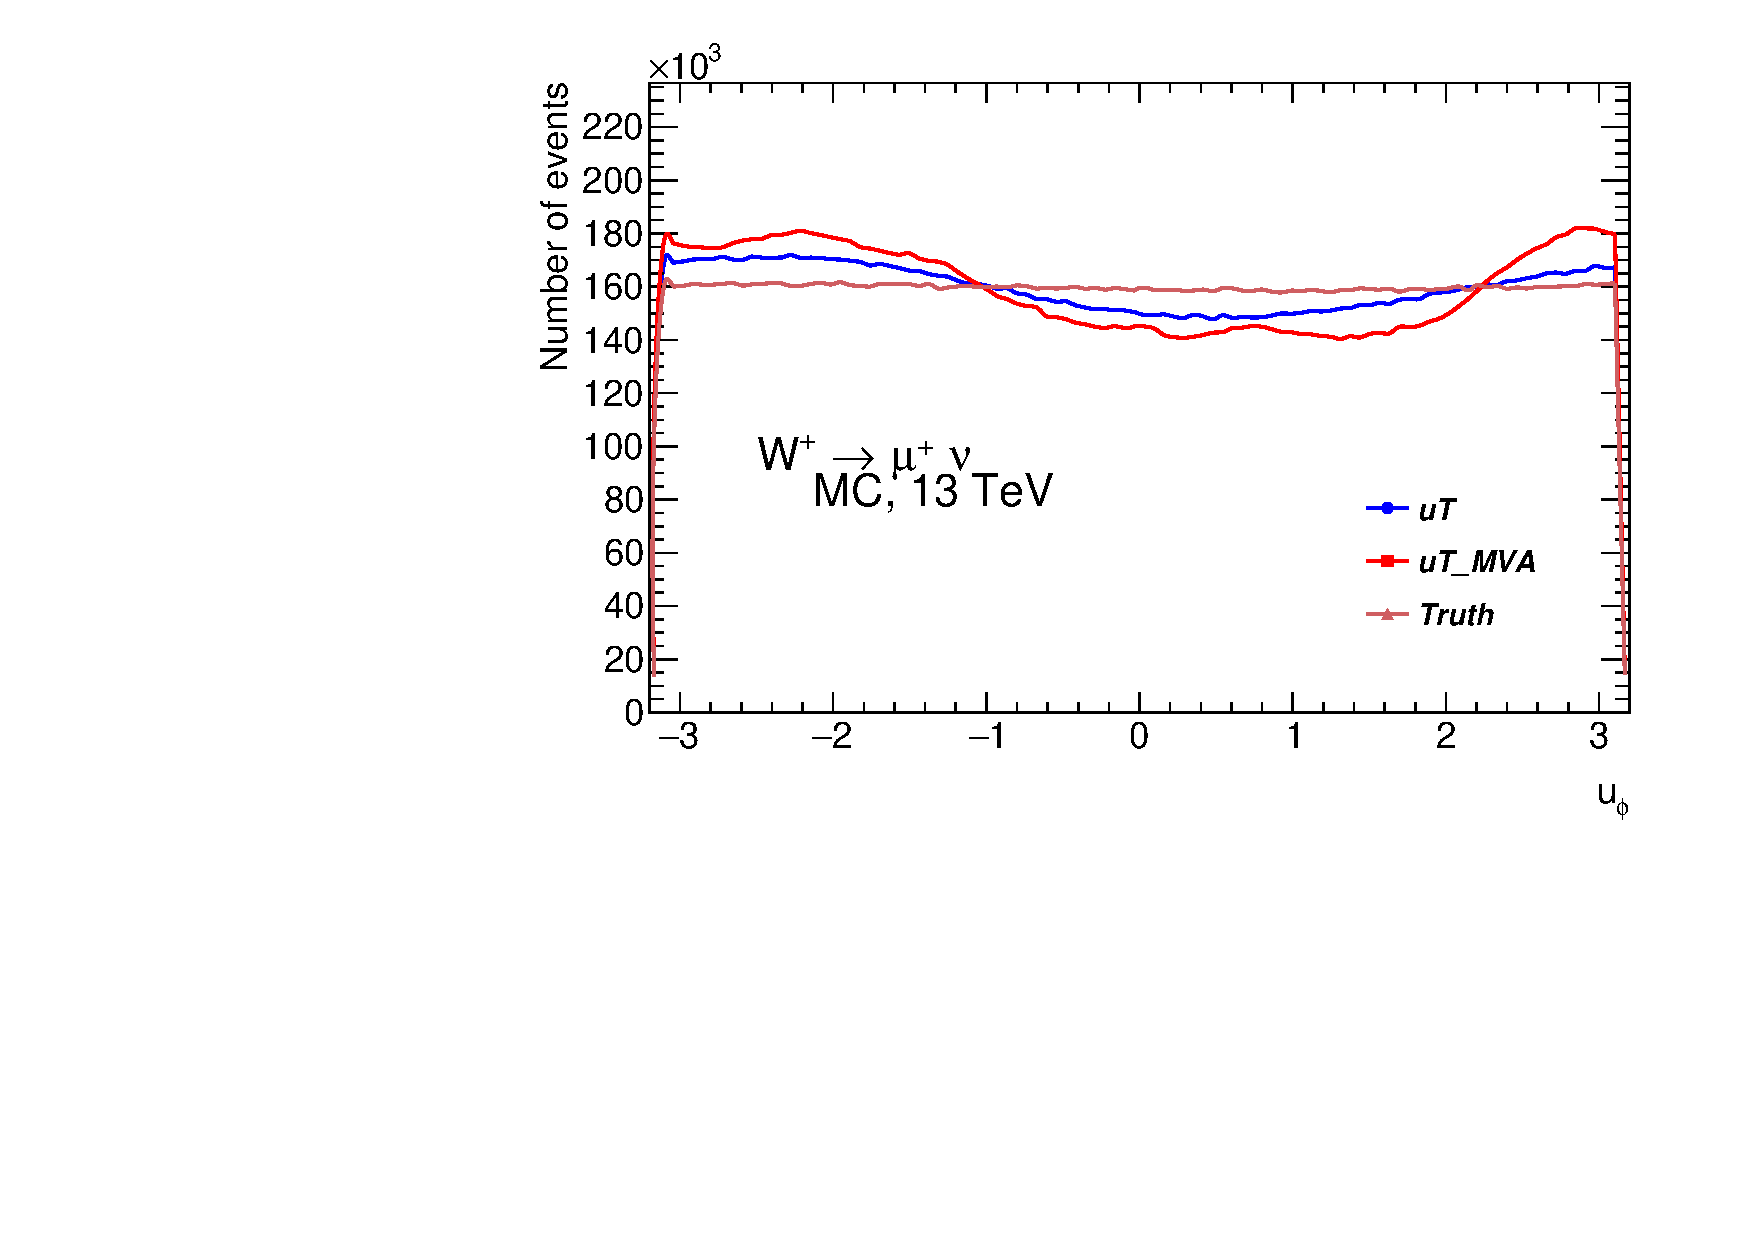
\includegraphics[width=.49\textwidth]{hist_uPhiplusmunu.pdf}}\\
    	{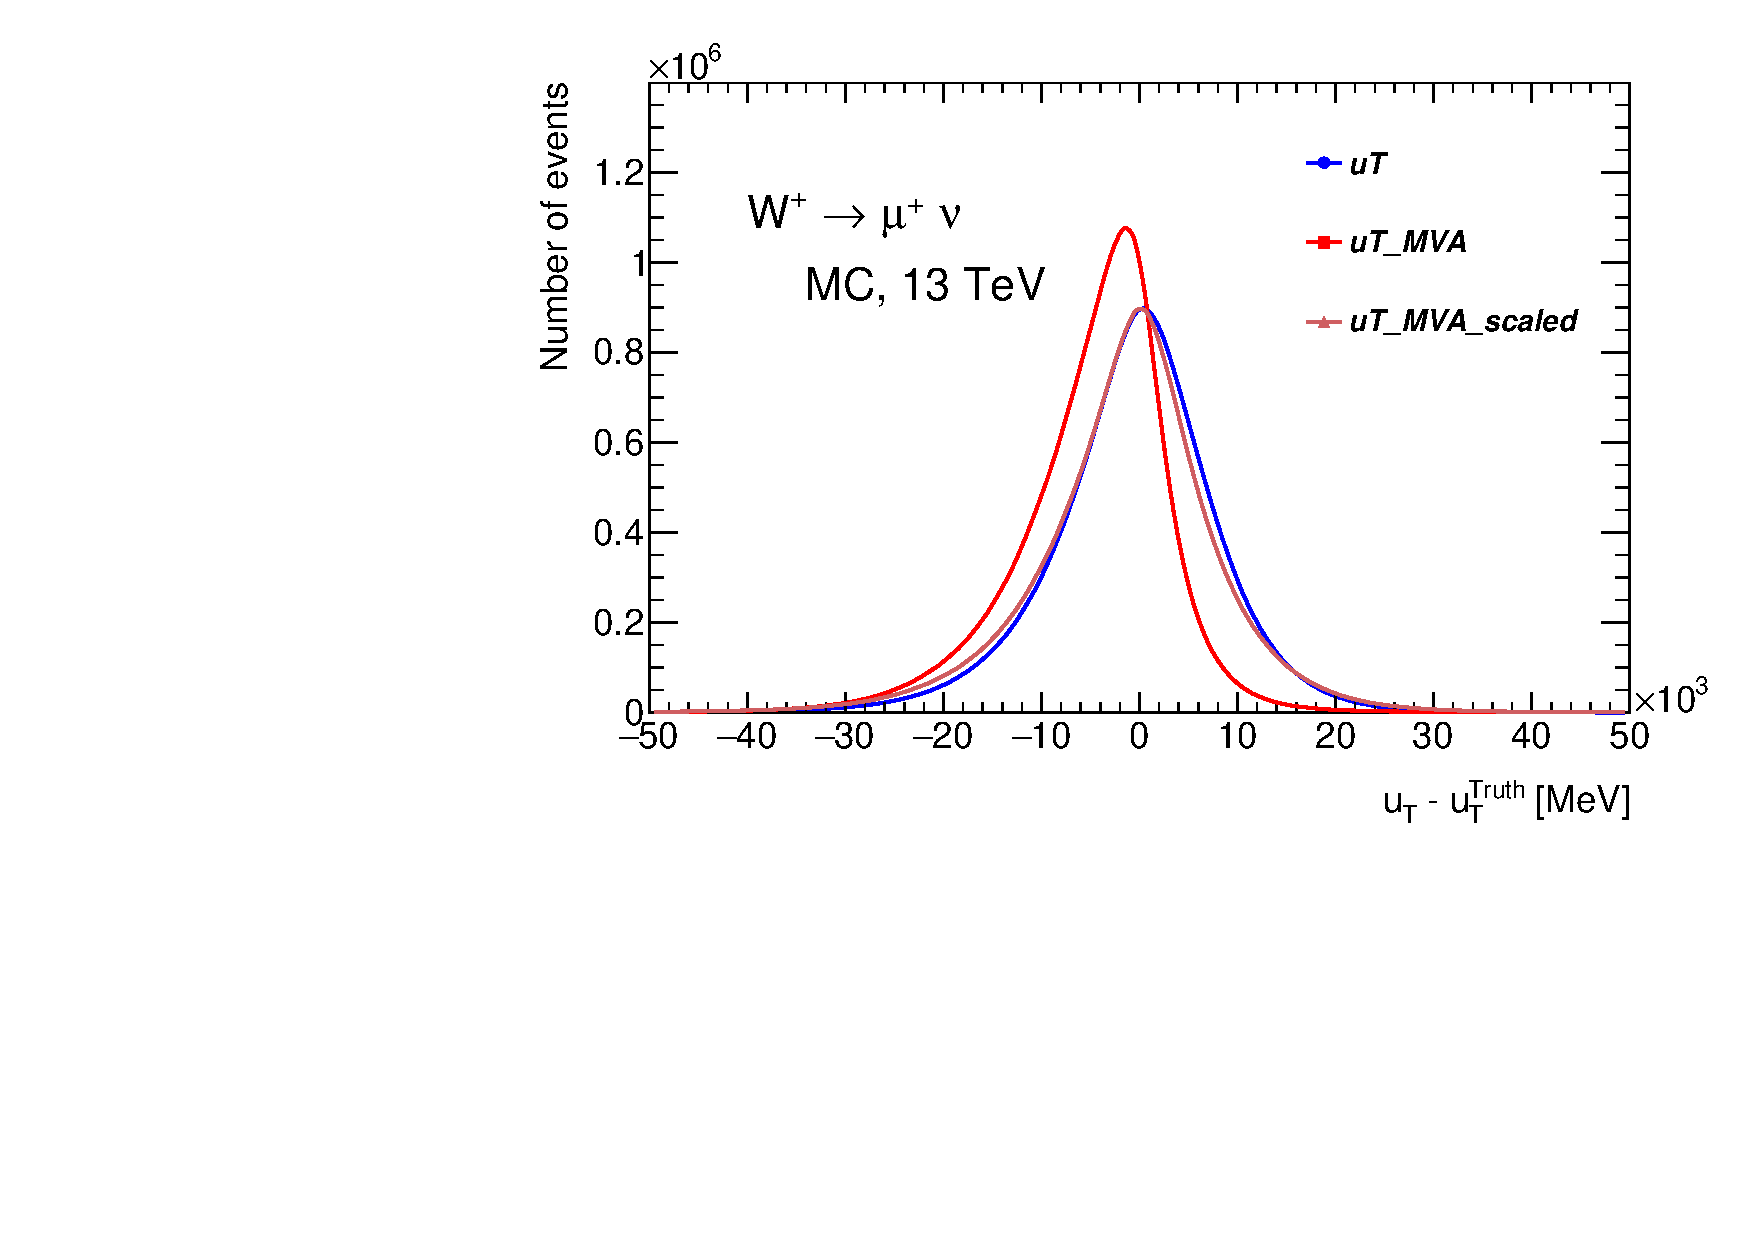
\includegraphics[width=.49\textwidth]{histosDeltaUtplusmunu.pdf}}
    	{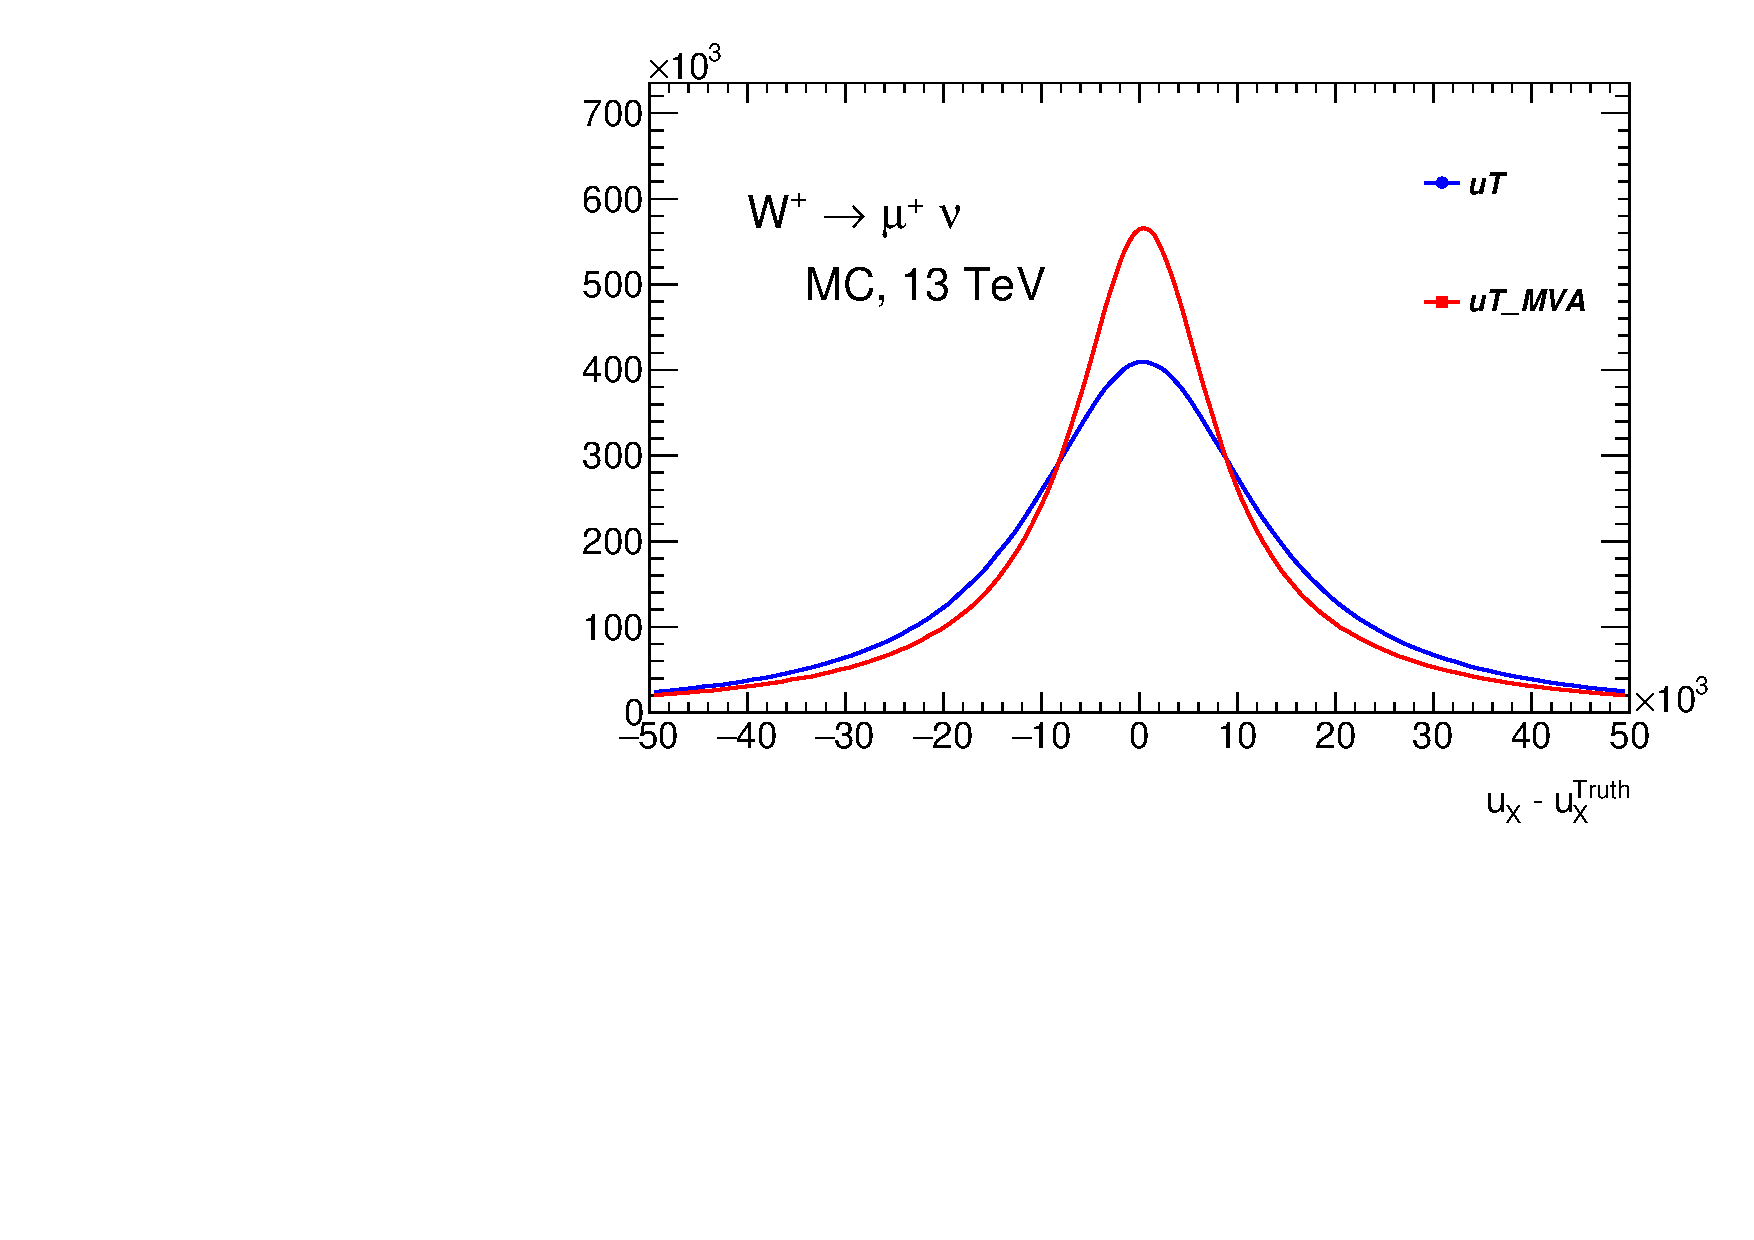
\includegraphics[width=.49\textwidth]{histosDeltaUxplusmunu.pdf}} \\
    	{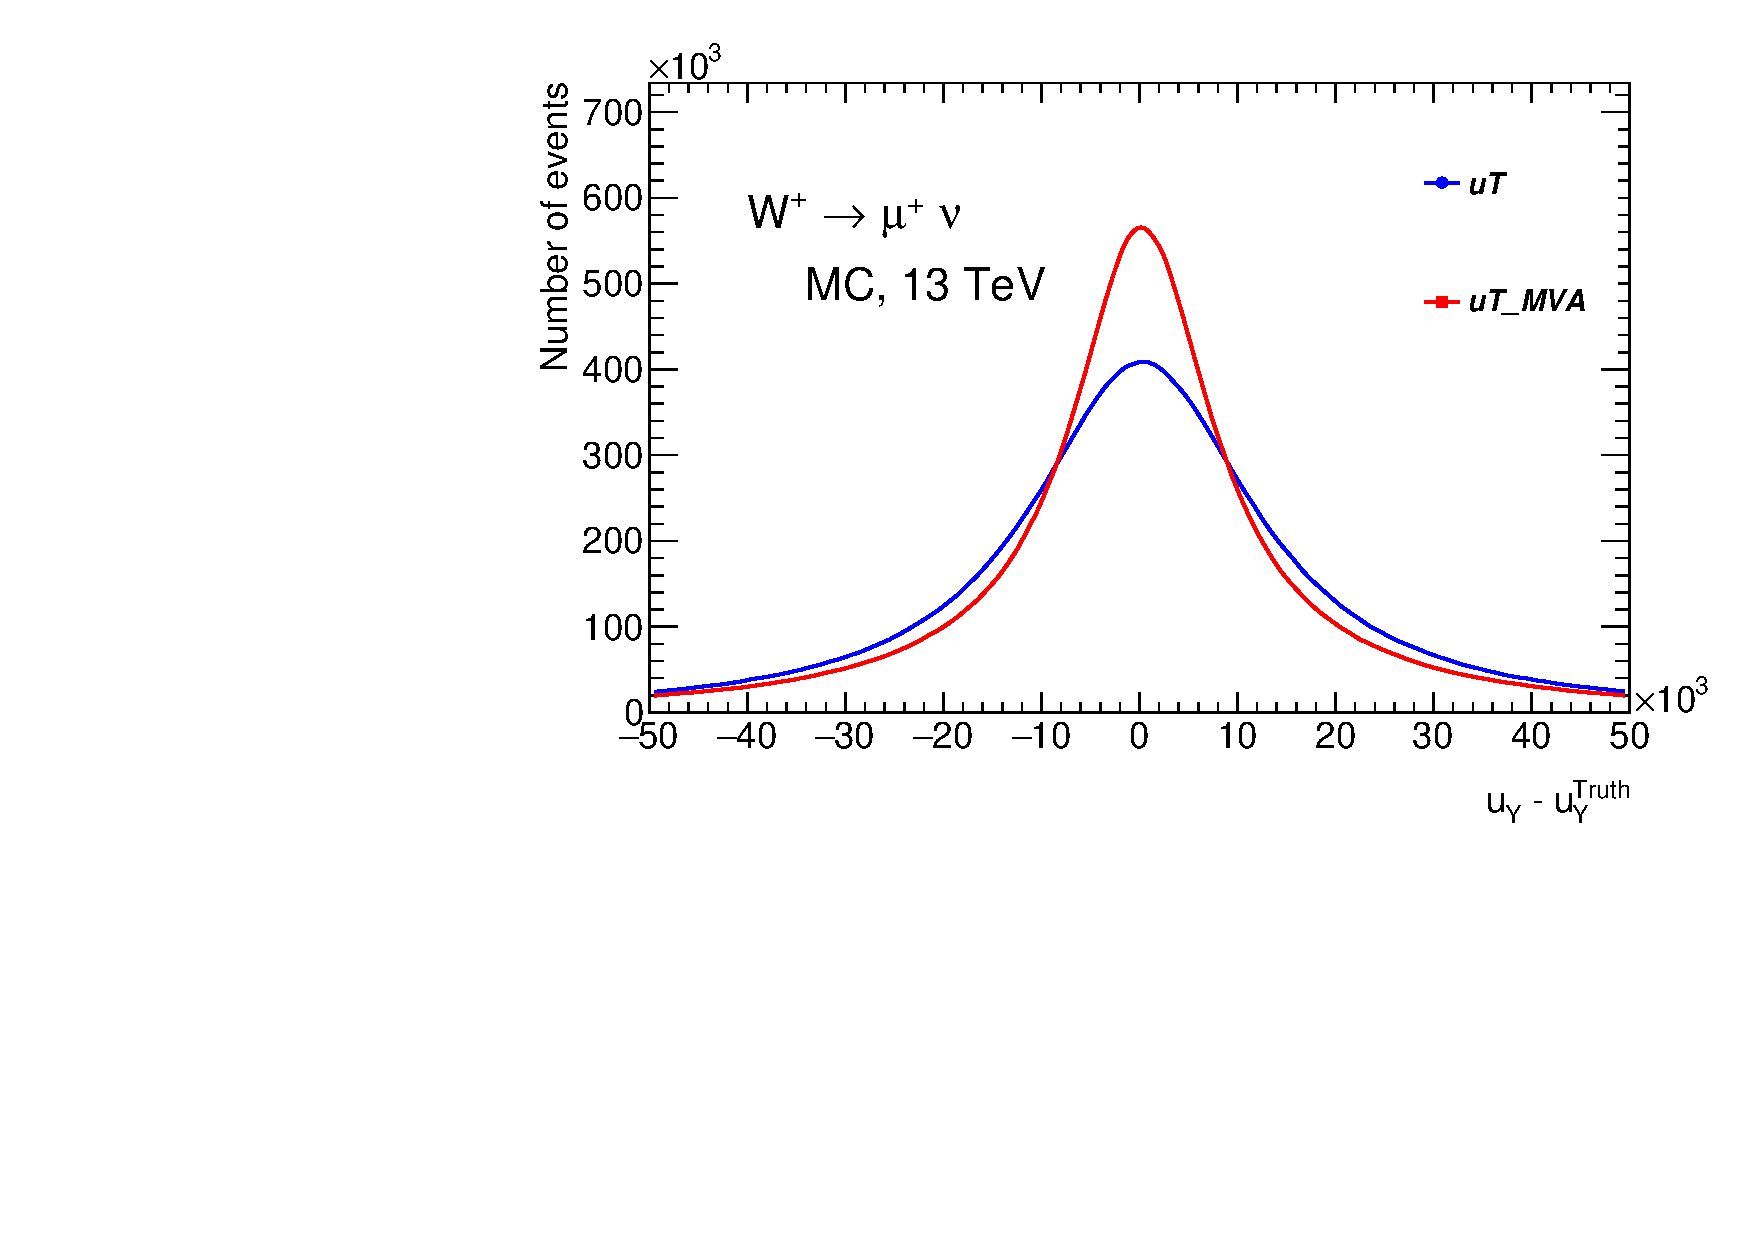
\includegraphics[width=.49\textwidth]{histosDeltaUyplusmunu.pdf}}
    	{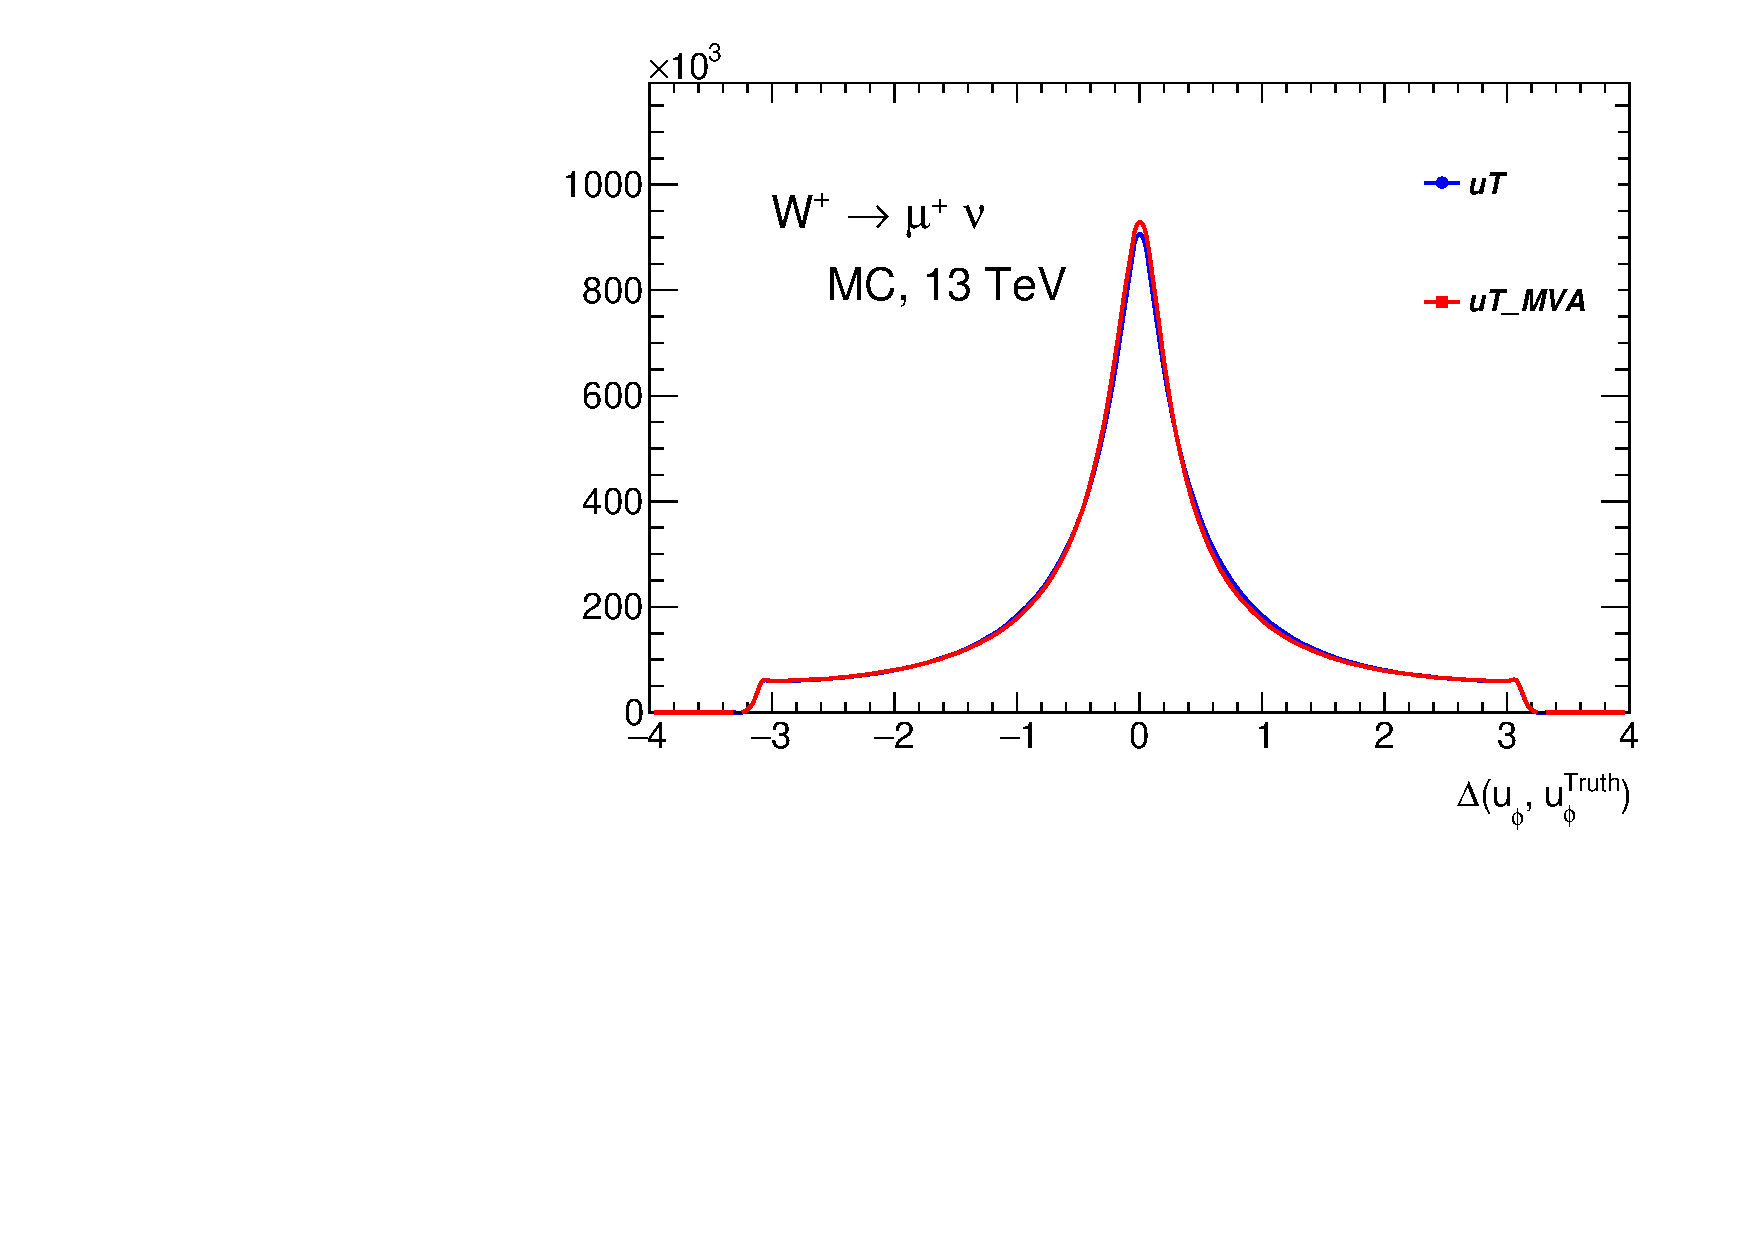
\includegraphics[width=.49\textwidth]{histosDeltaUPhiplusmunu.pdf}}\\
    	\label{fig:plusmunu_data_distributions1}
    \end{figure}
    \begin{figure}[h]
    	\centering
    	{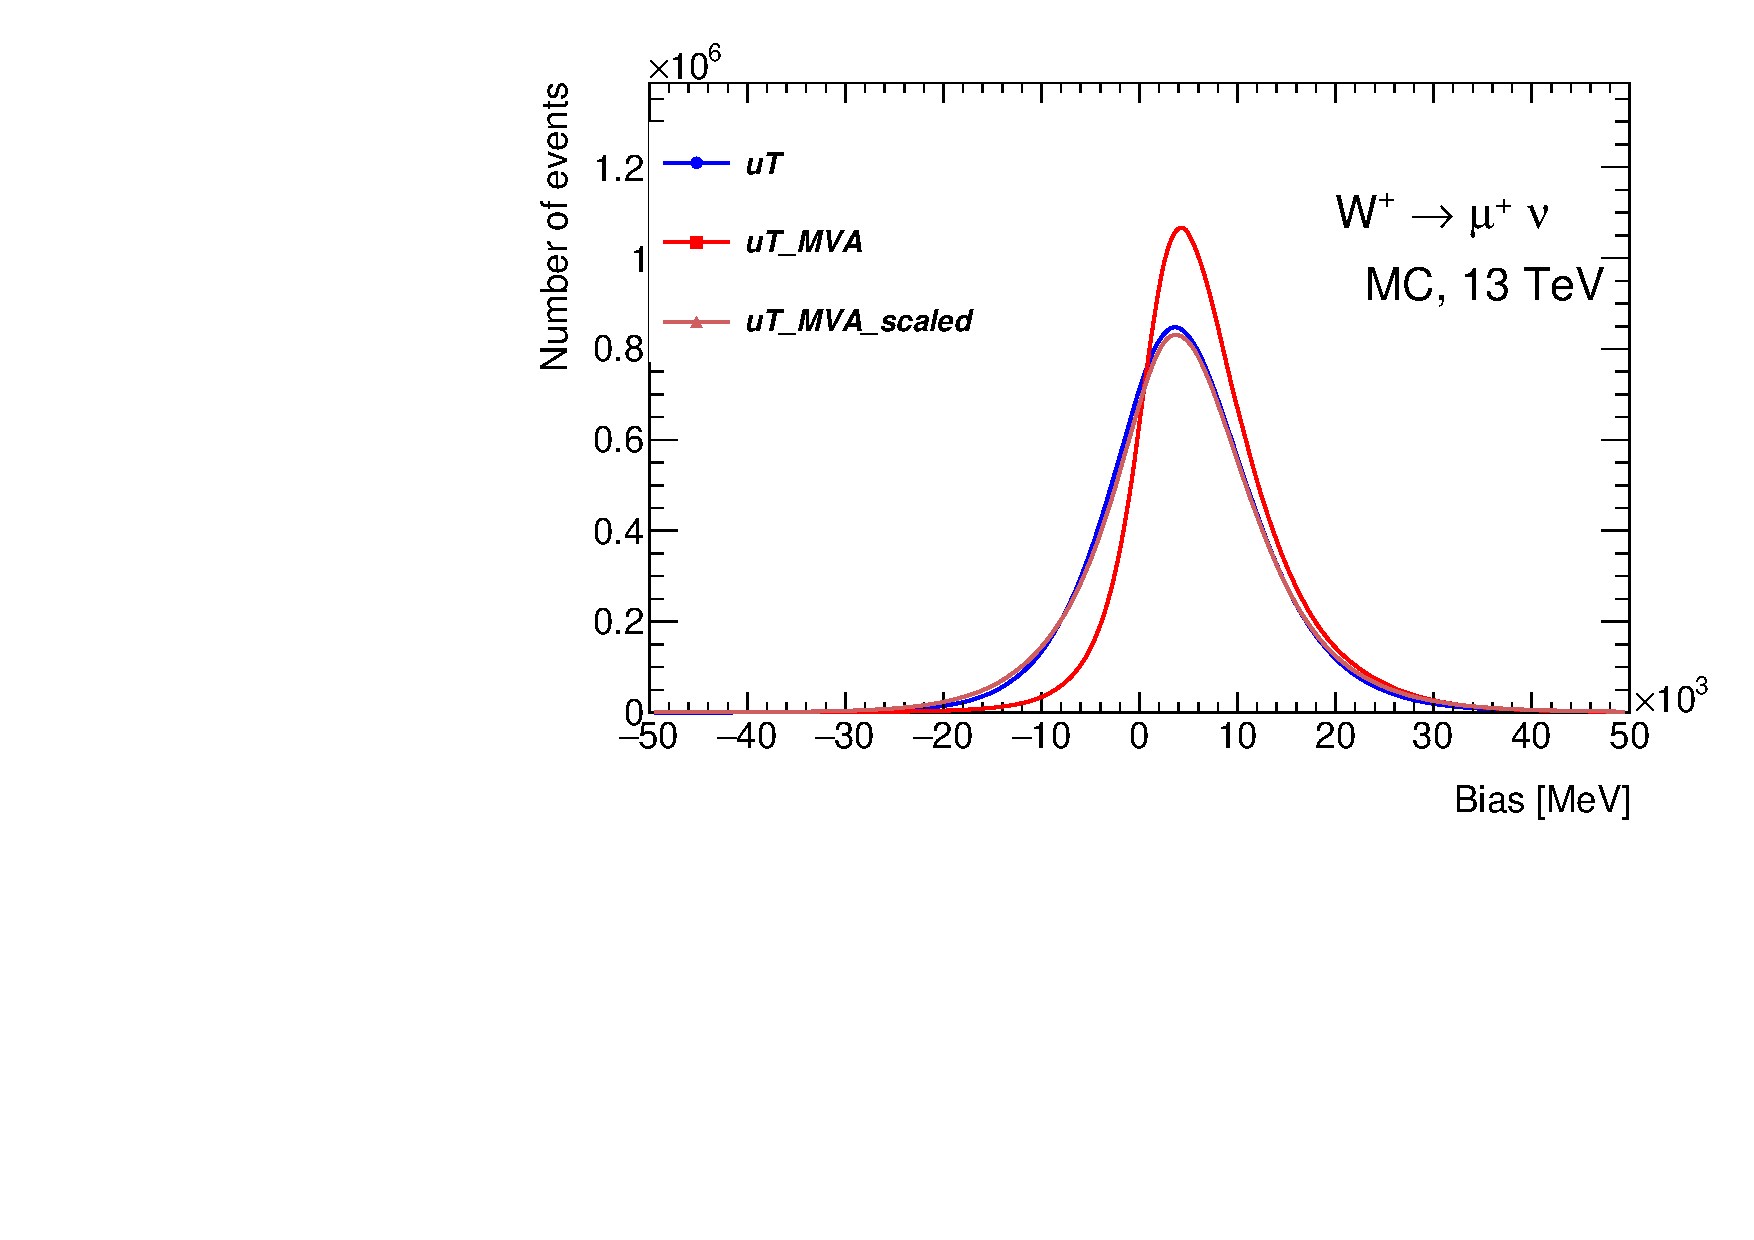
\includegraphics[width=.49\textwidth]{outMVA_biasplusmunu}}
    	{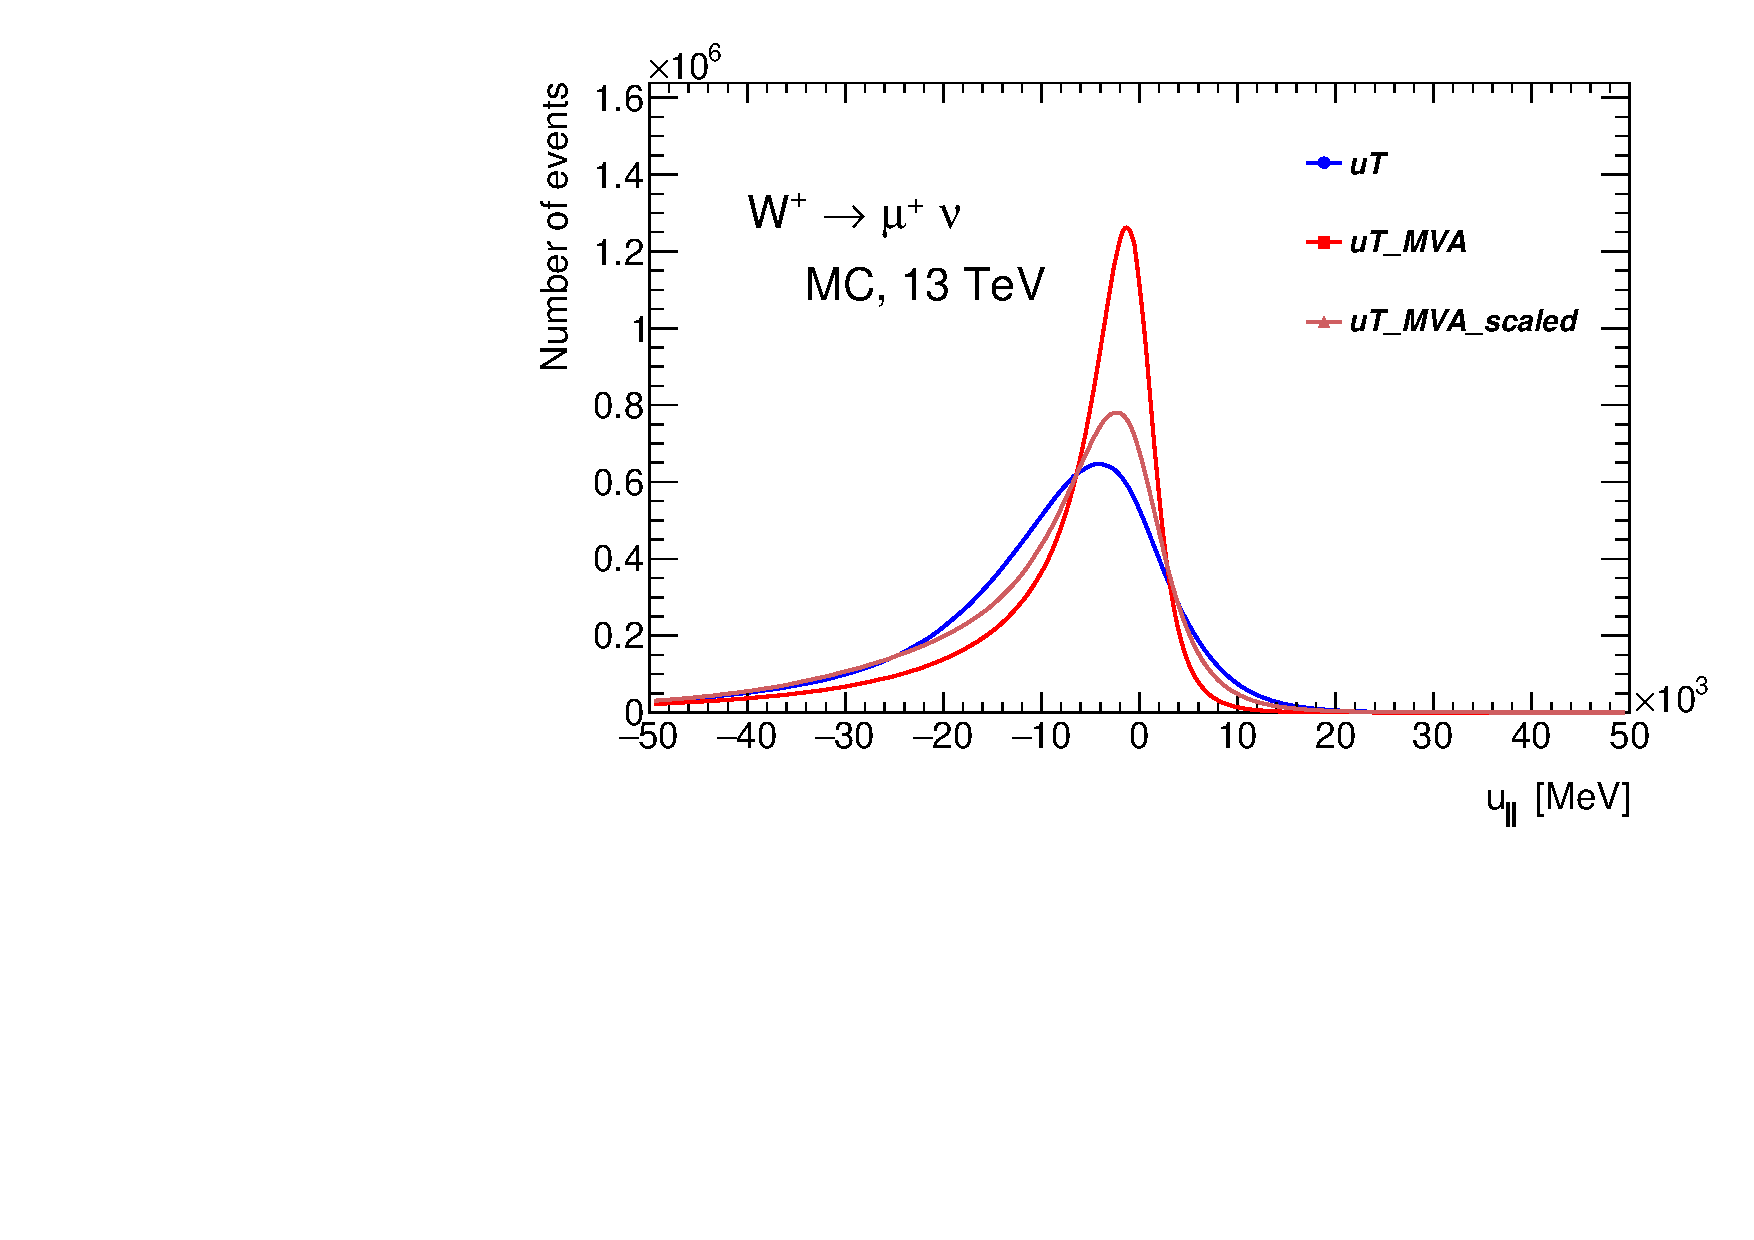
\includegraphics[width=.49\textwidth]{outMVA_Uparplusmunu}}
    	{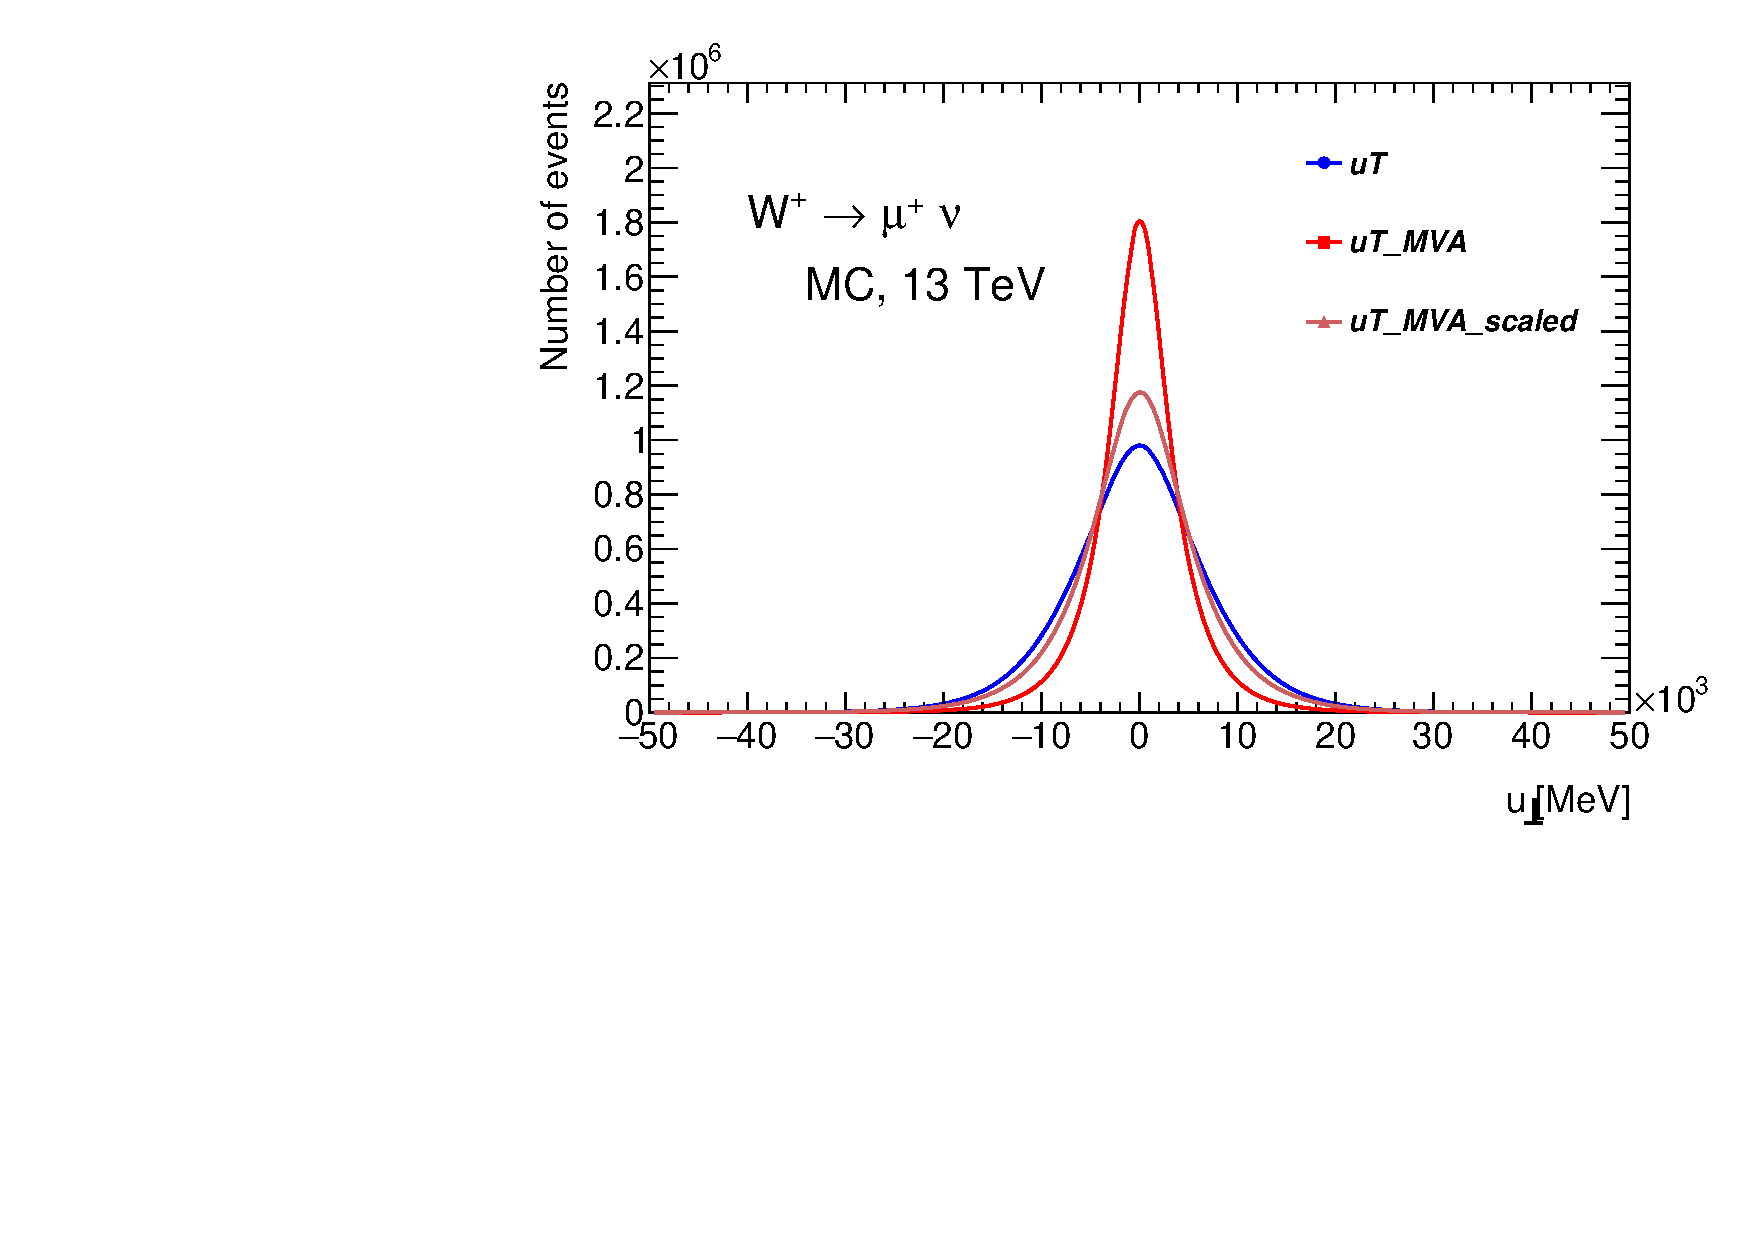
\includegraphics[width=.49\textwidth]{outMVA_uPerpplusmunu}}
    	{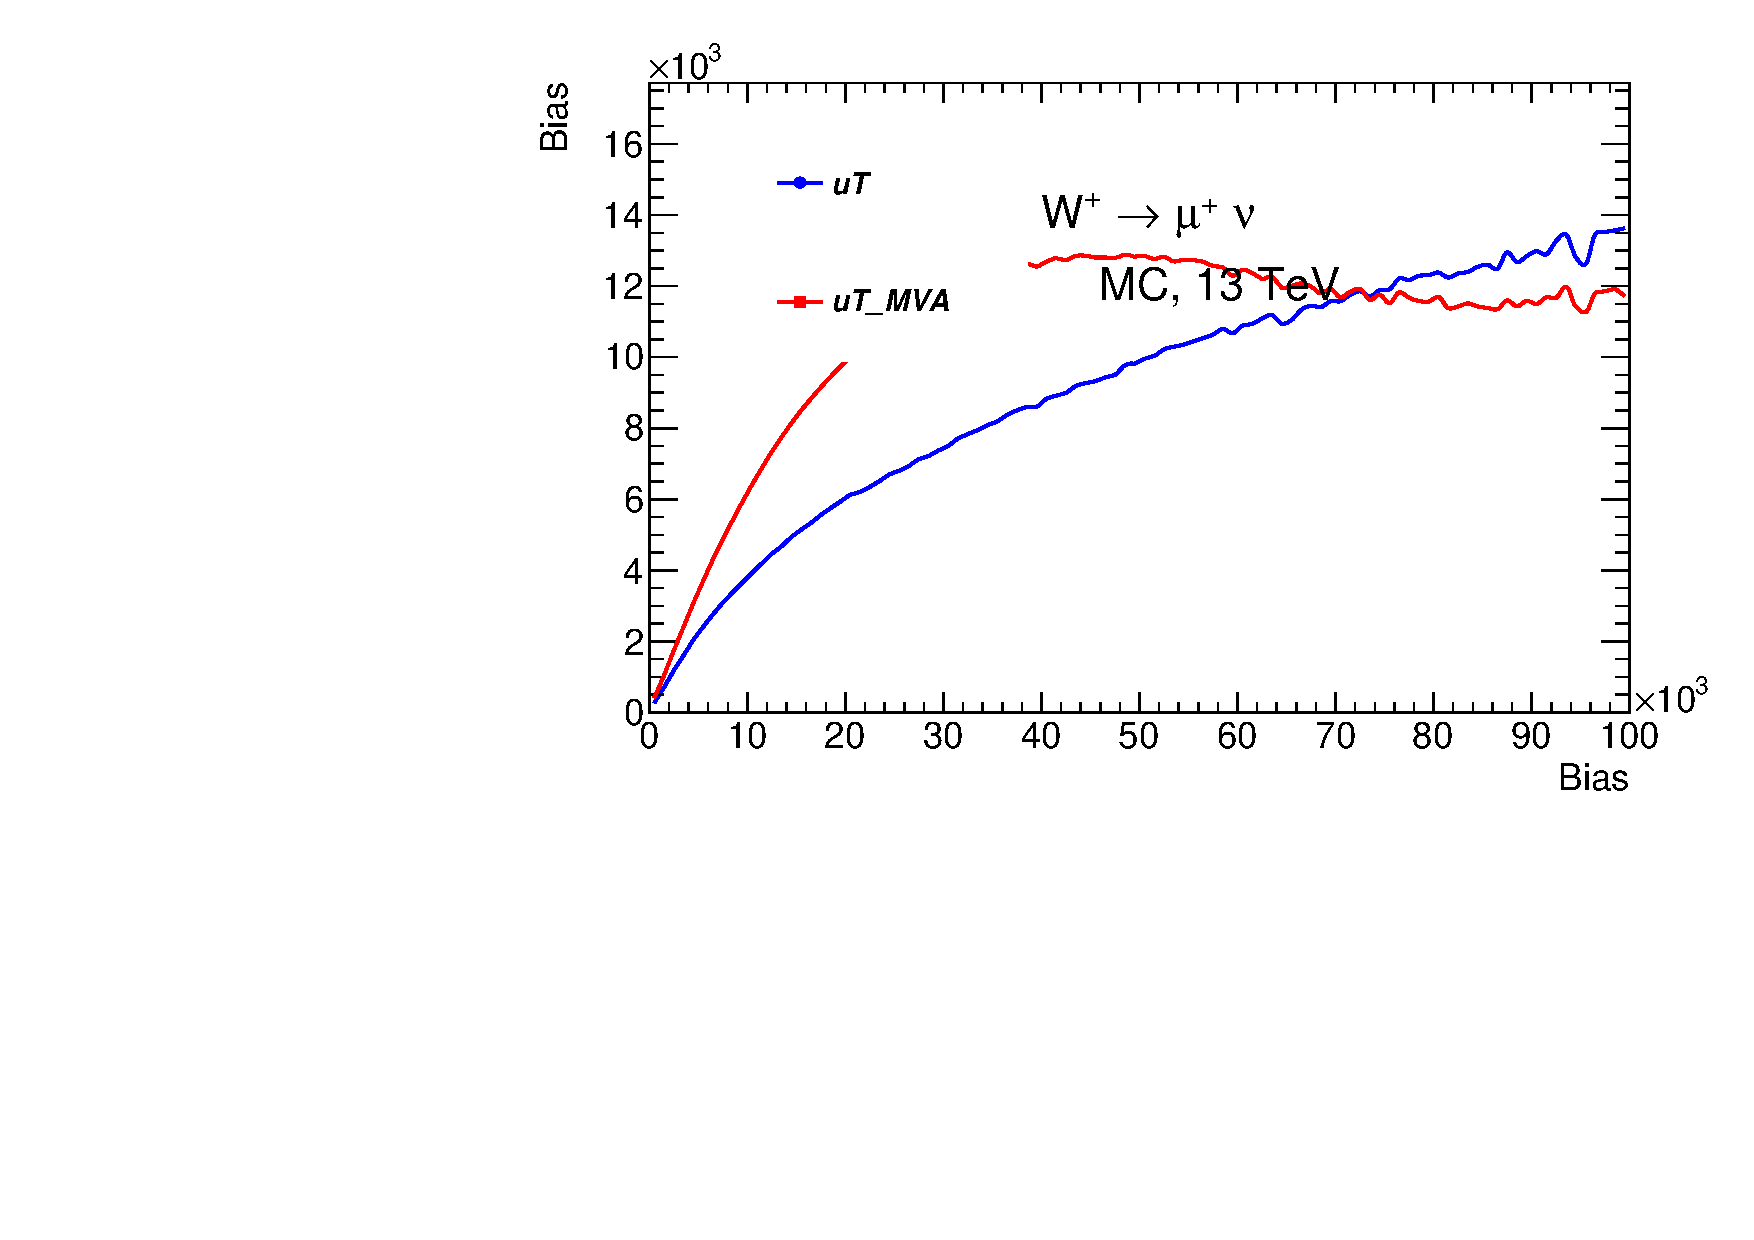
\includegraphics[width=.49\textwidth]{histosMeanBiasplusmunu}}
    	{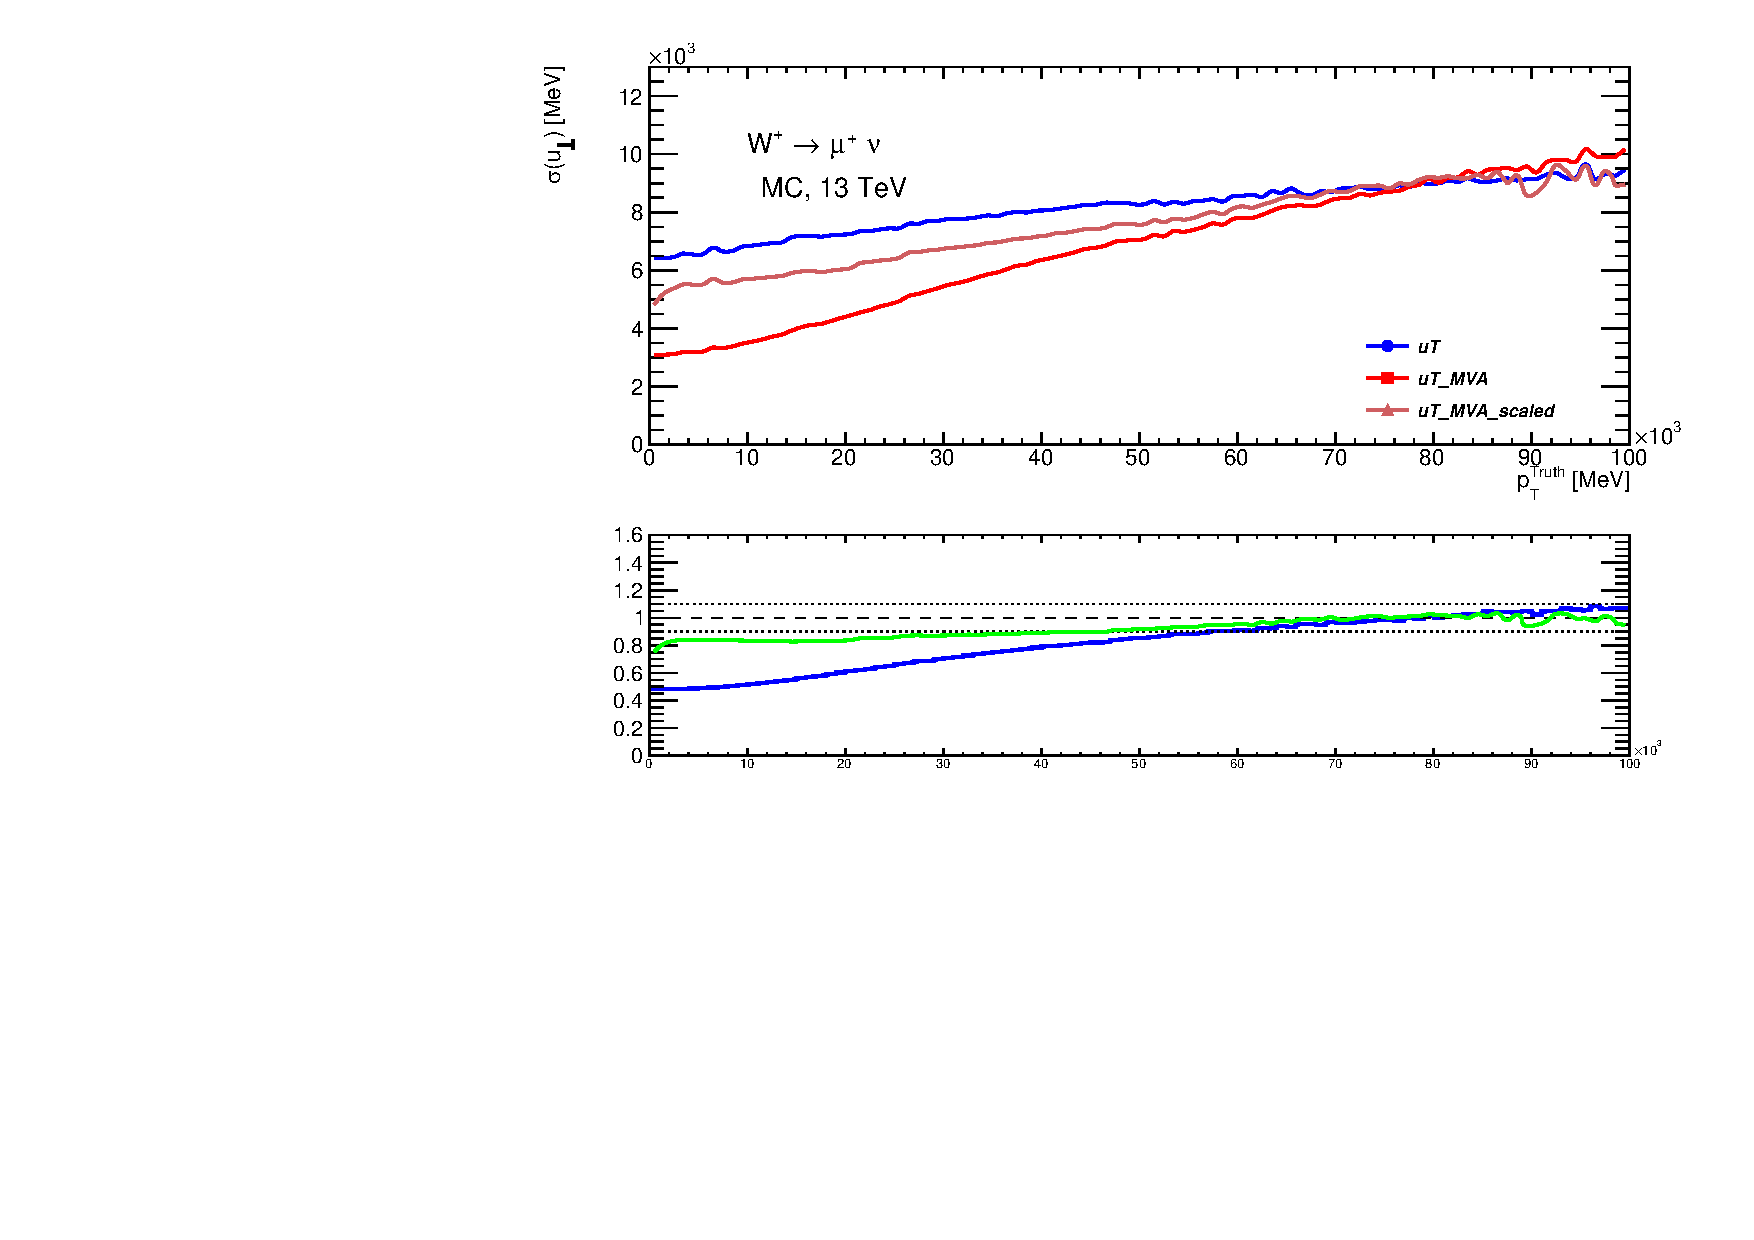
\includegraphics[width=.49\textwidth]{histosSigmaUperpplusmunu}}
    	{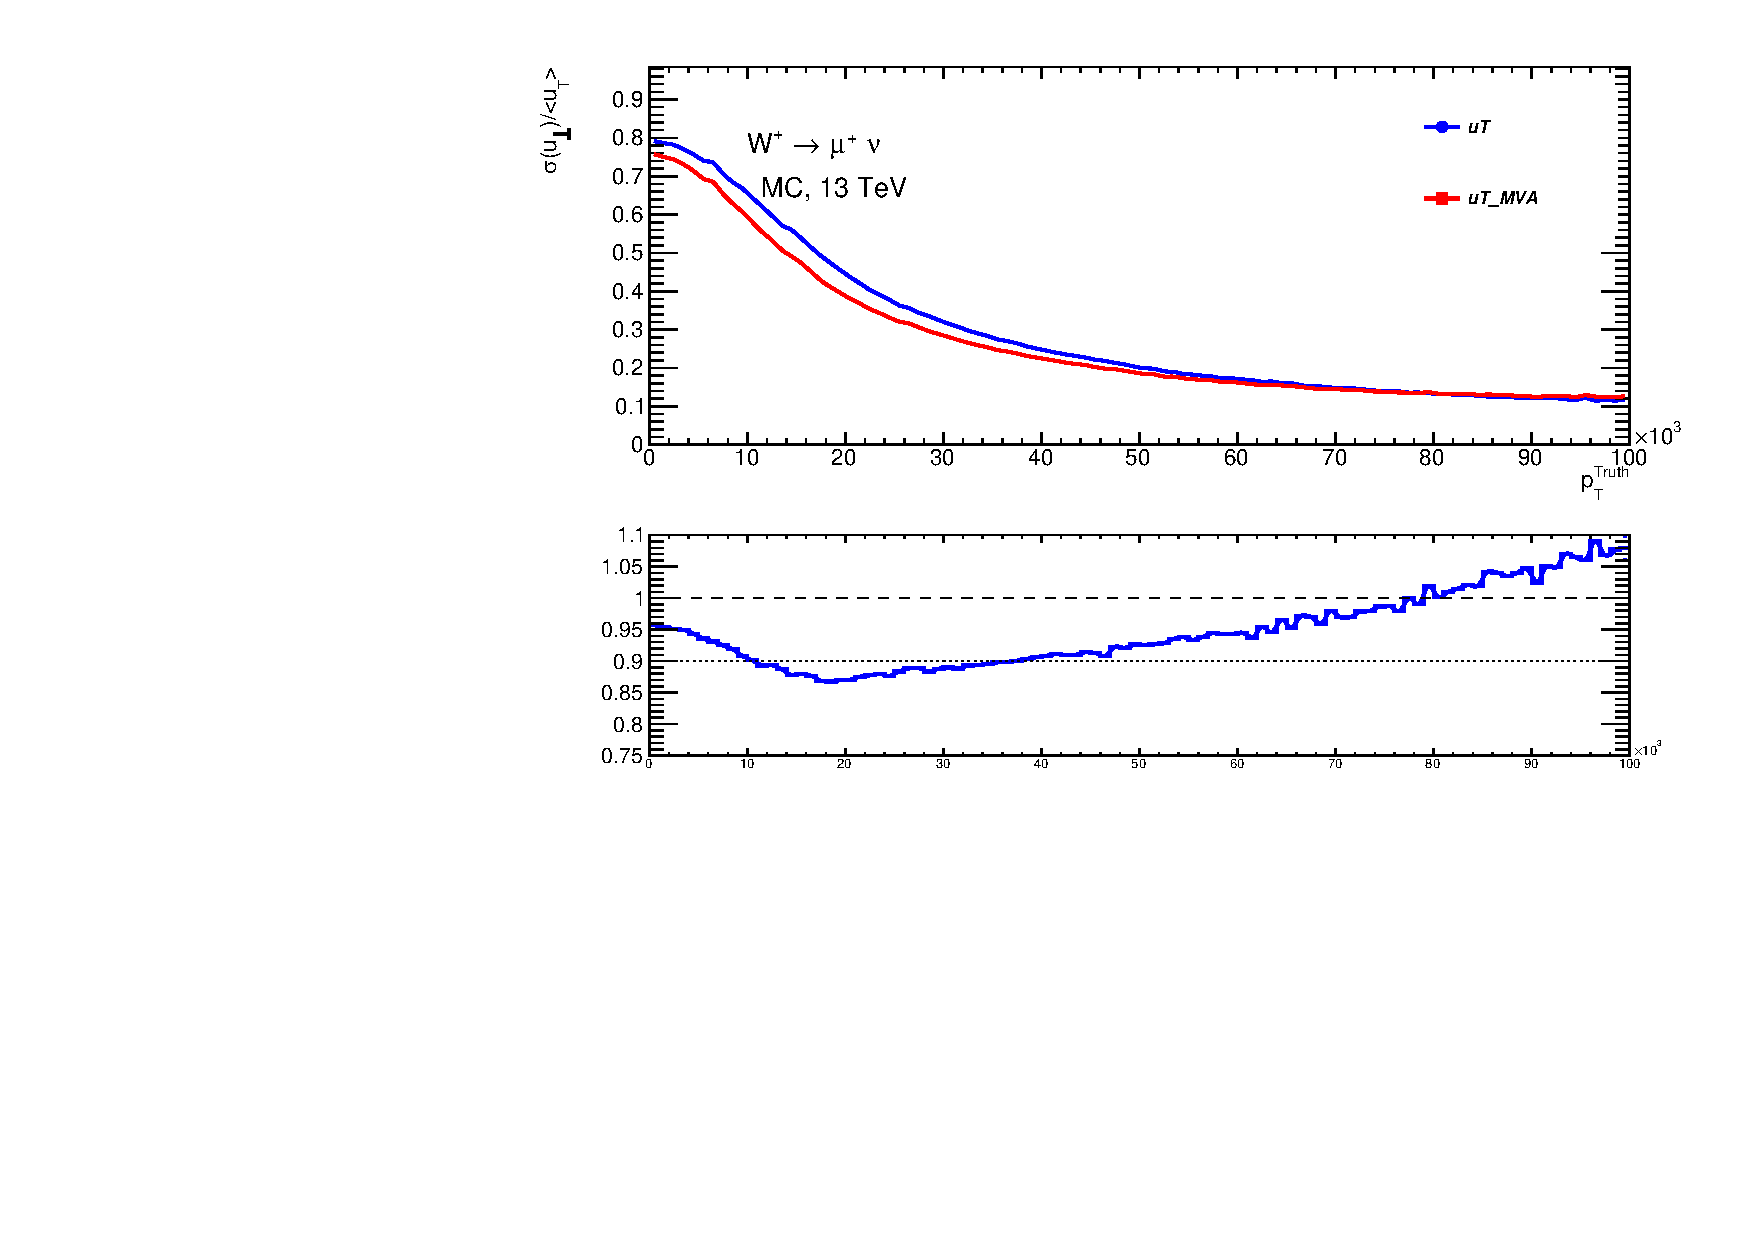
\includegraphics[width=.49\textwidth]{histosUperpRelativeplusmunu}}
    	\caption{Comparison of kinematic distributions of $u_T$ vs $u_T^{MVA}$ for $W^-\rightarrow e^-\nu$ data sample.}
    	\label{fig:plusmunu_data_distributions2}
    \end{figure}
    
        \begin{figure}[h]
    	\centering
    	{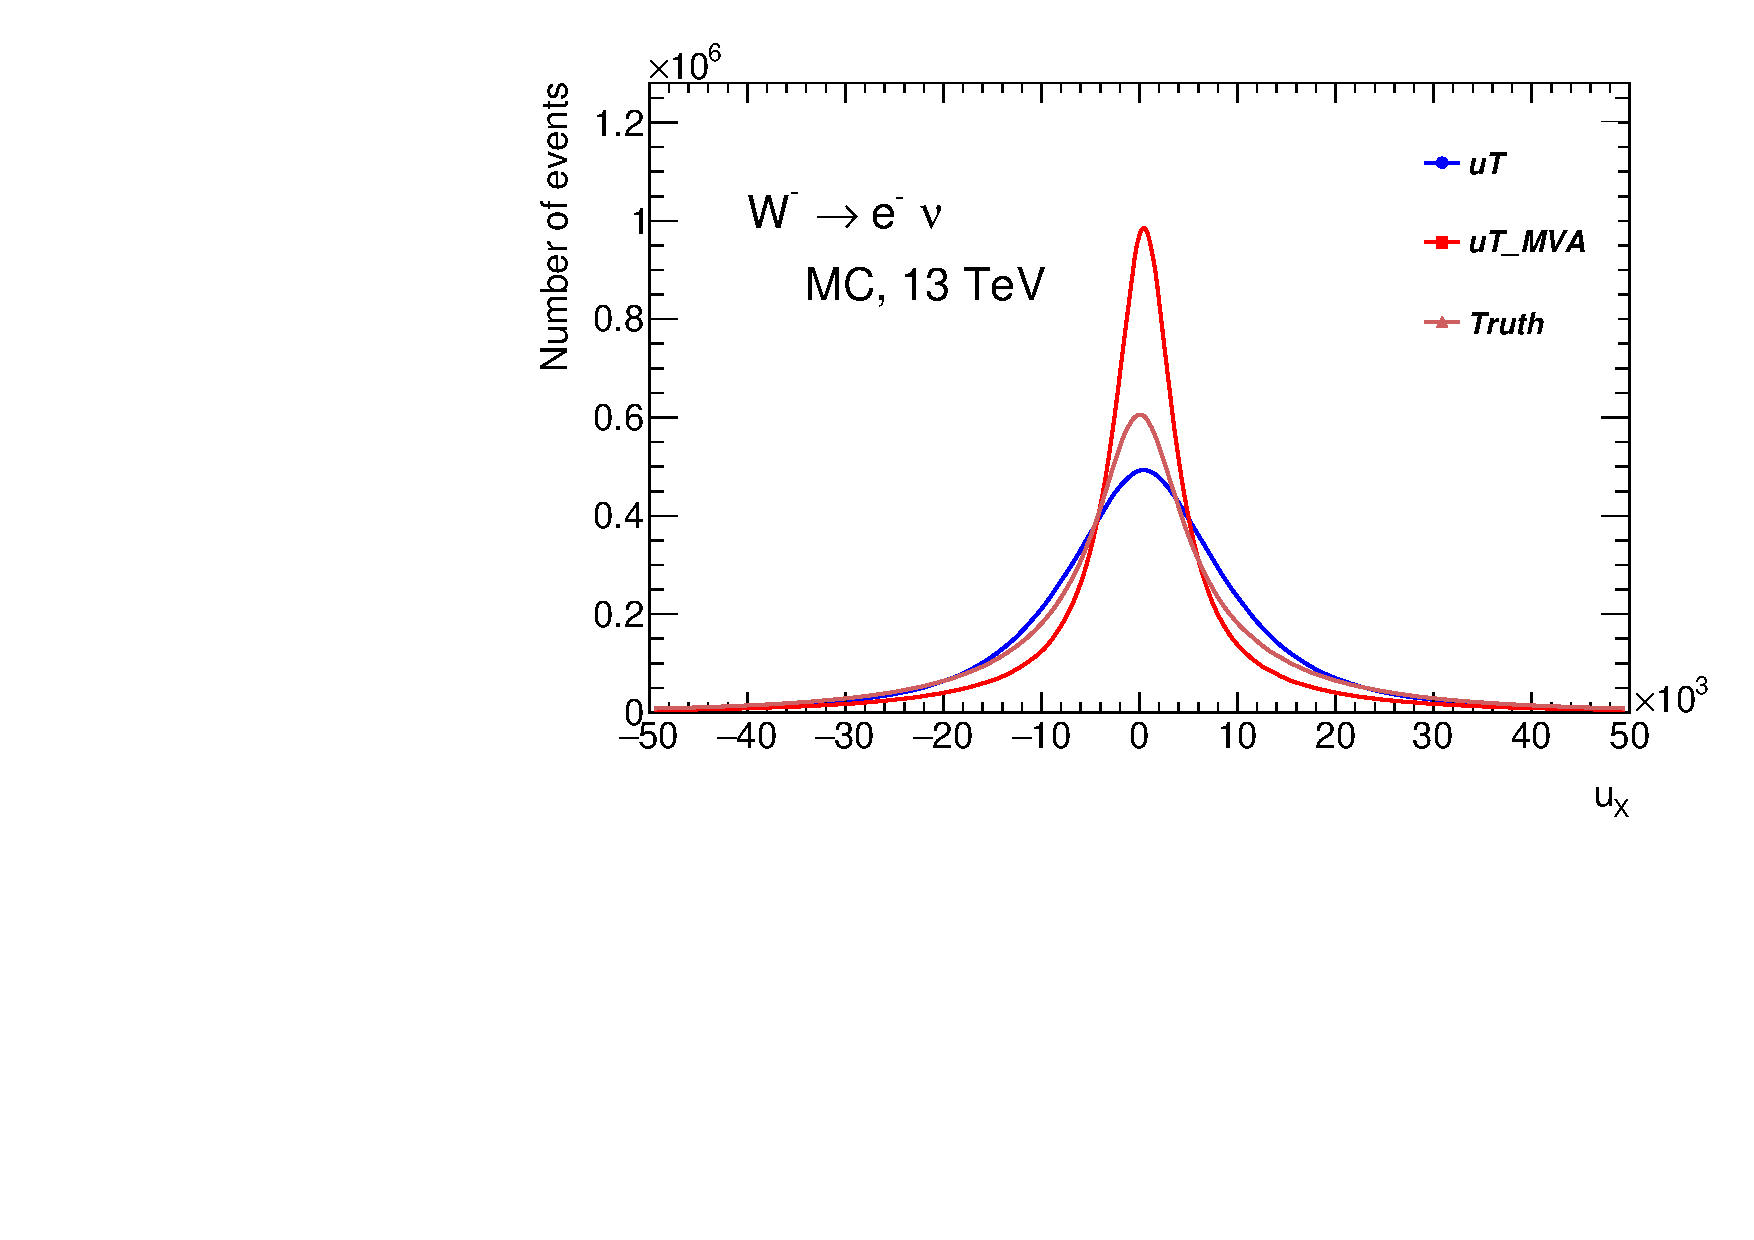
\includegraphics[width=.49\textwidth]{hist_uXminusenu.pdf}}
    	{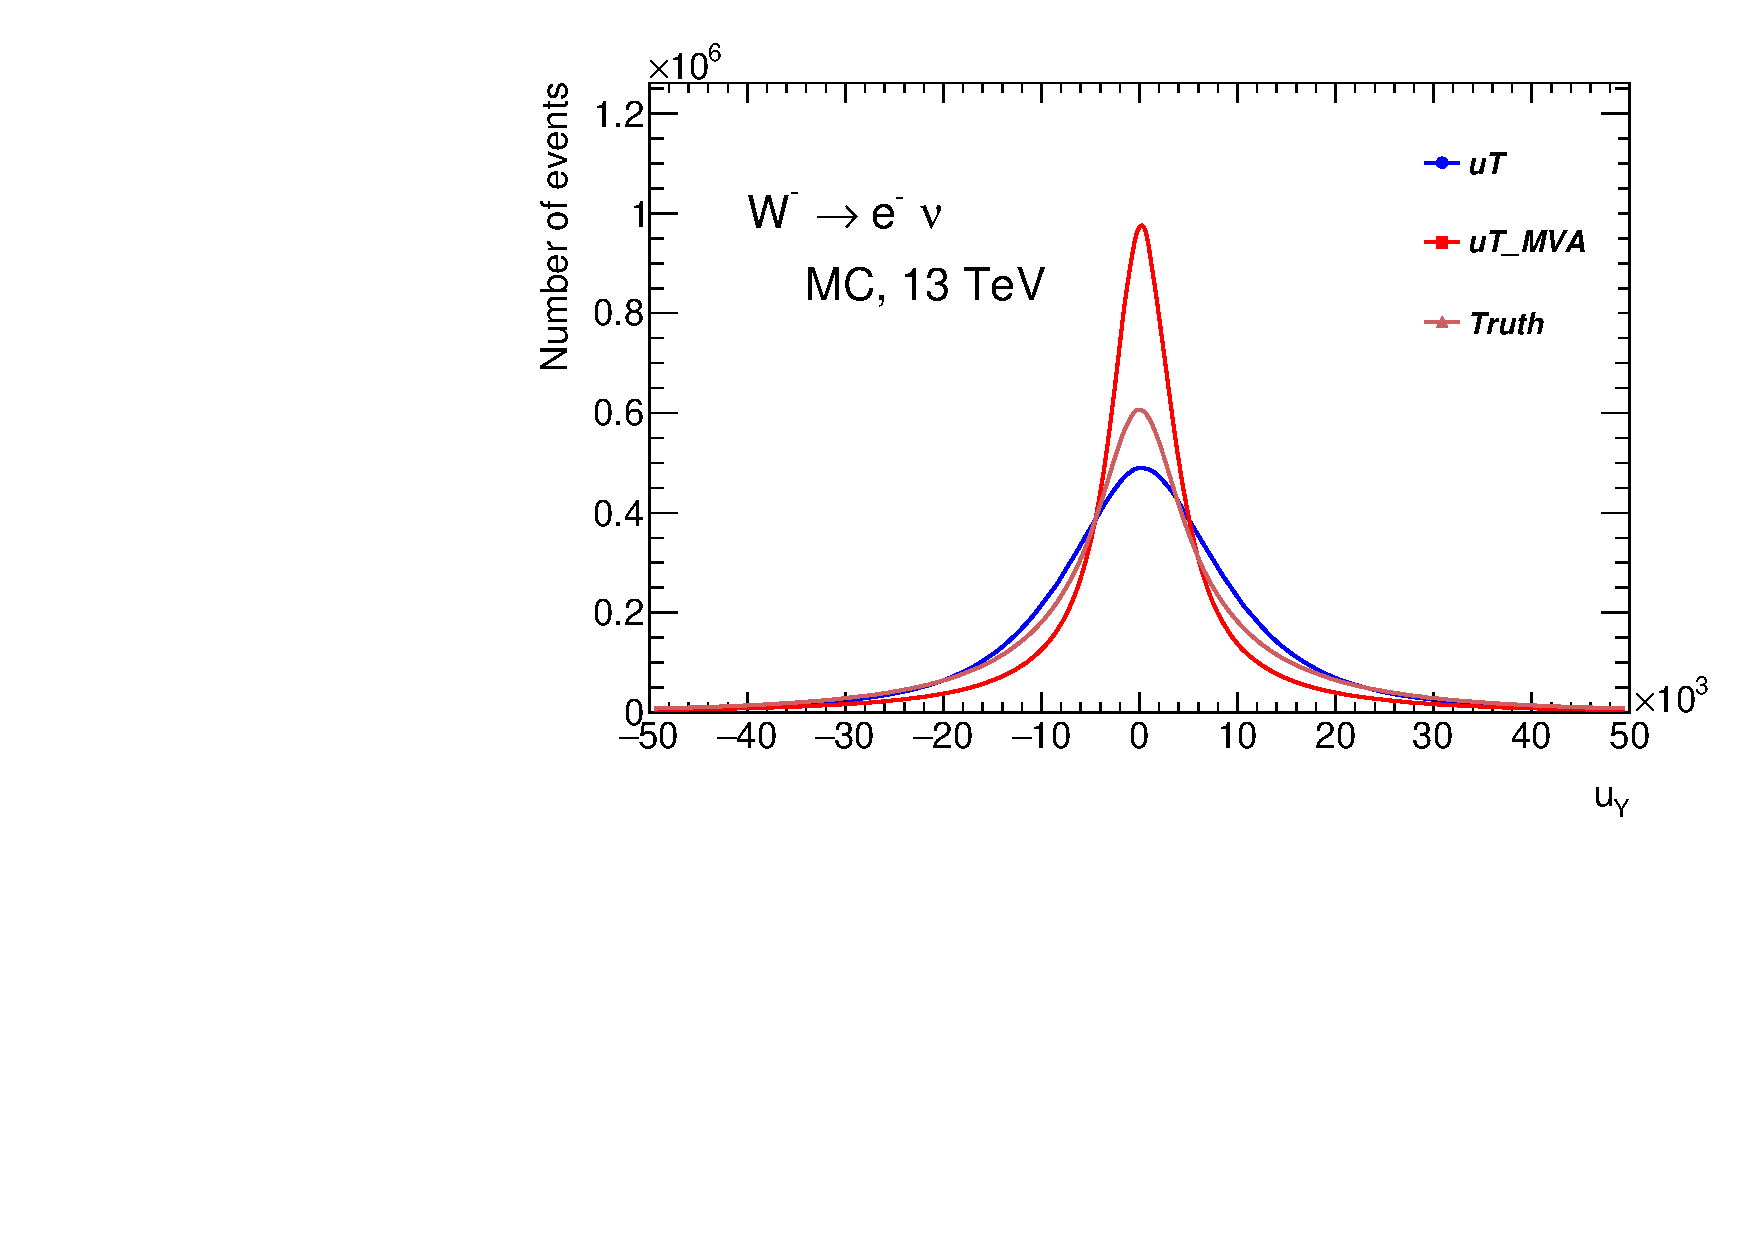
\includegraphics[width=.49\textwidth]{hist_uYminusenu.pdf}} \\
    	{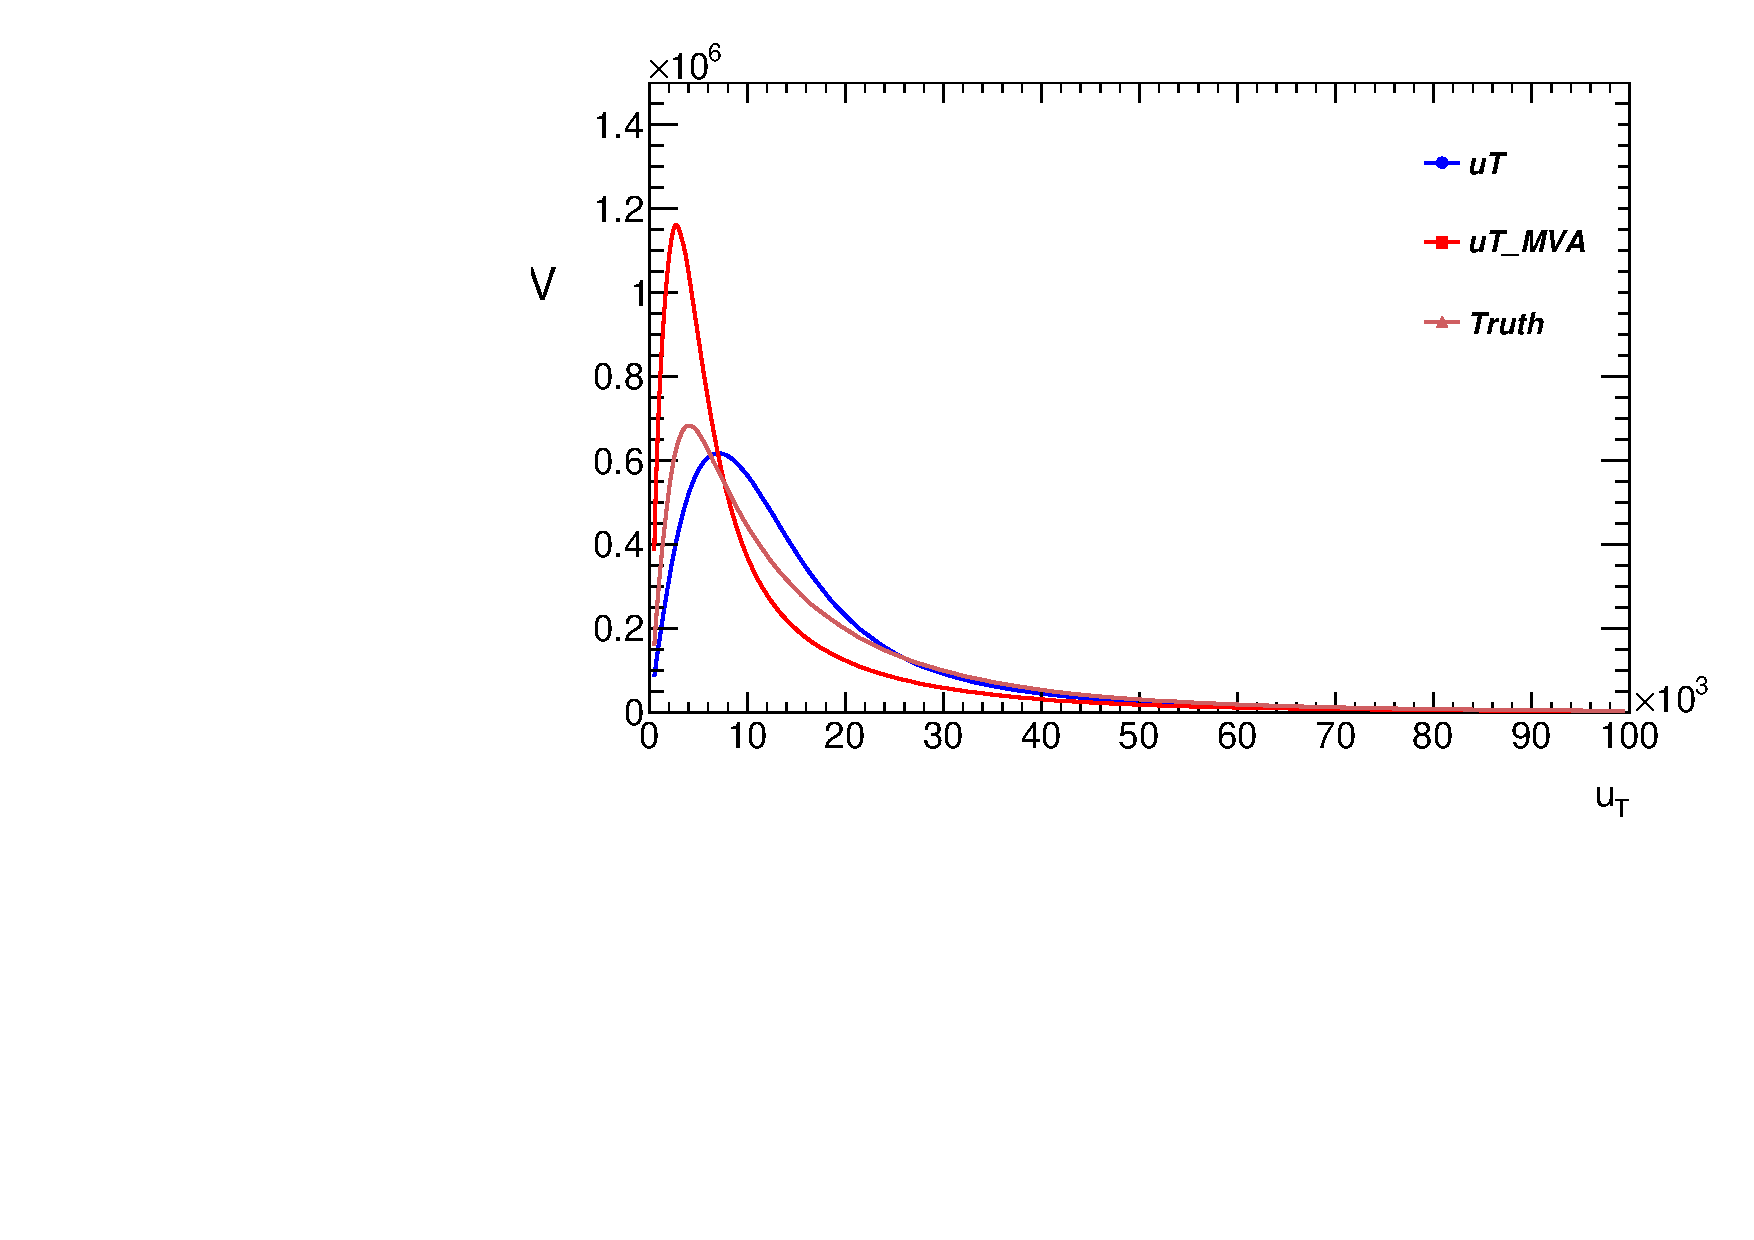
\includegraphics[width=.49\textwidth]{hist_uTminusenu.pdf}}
    	{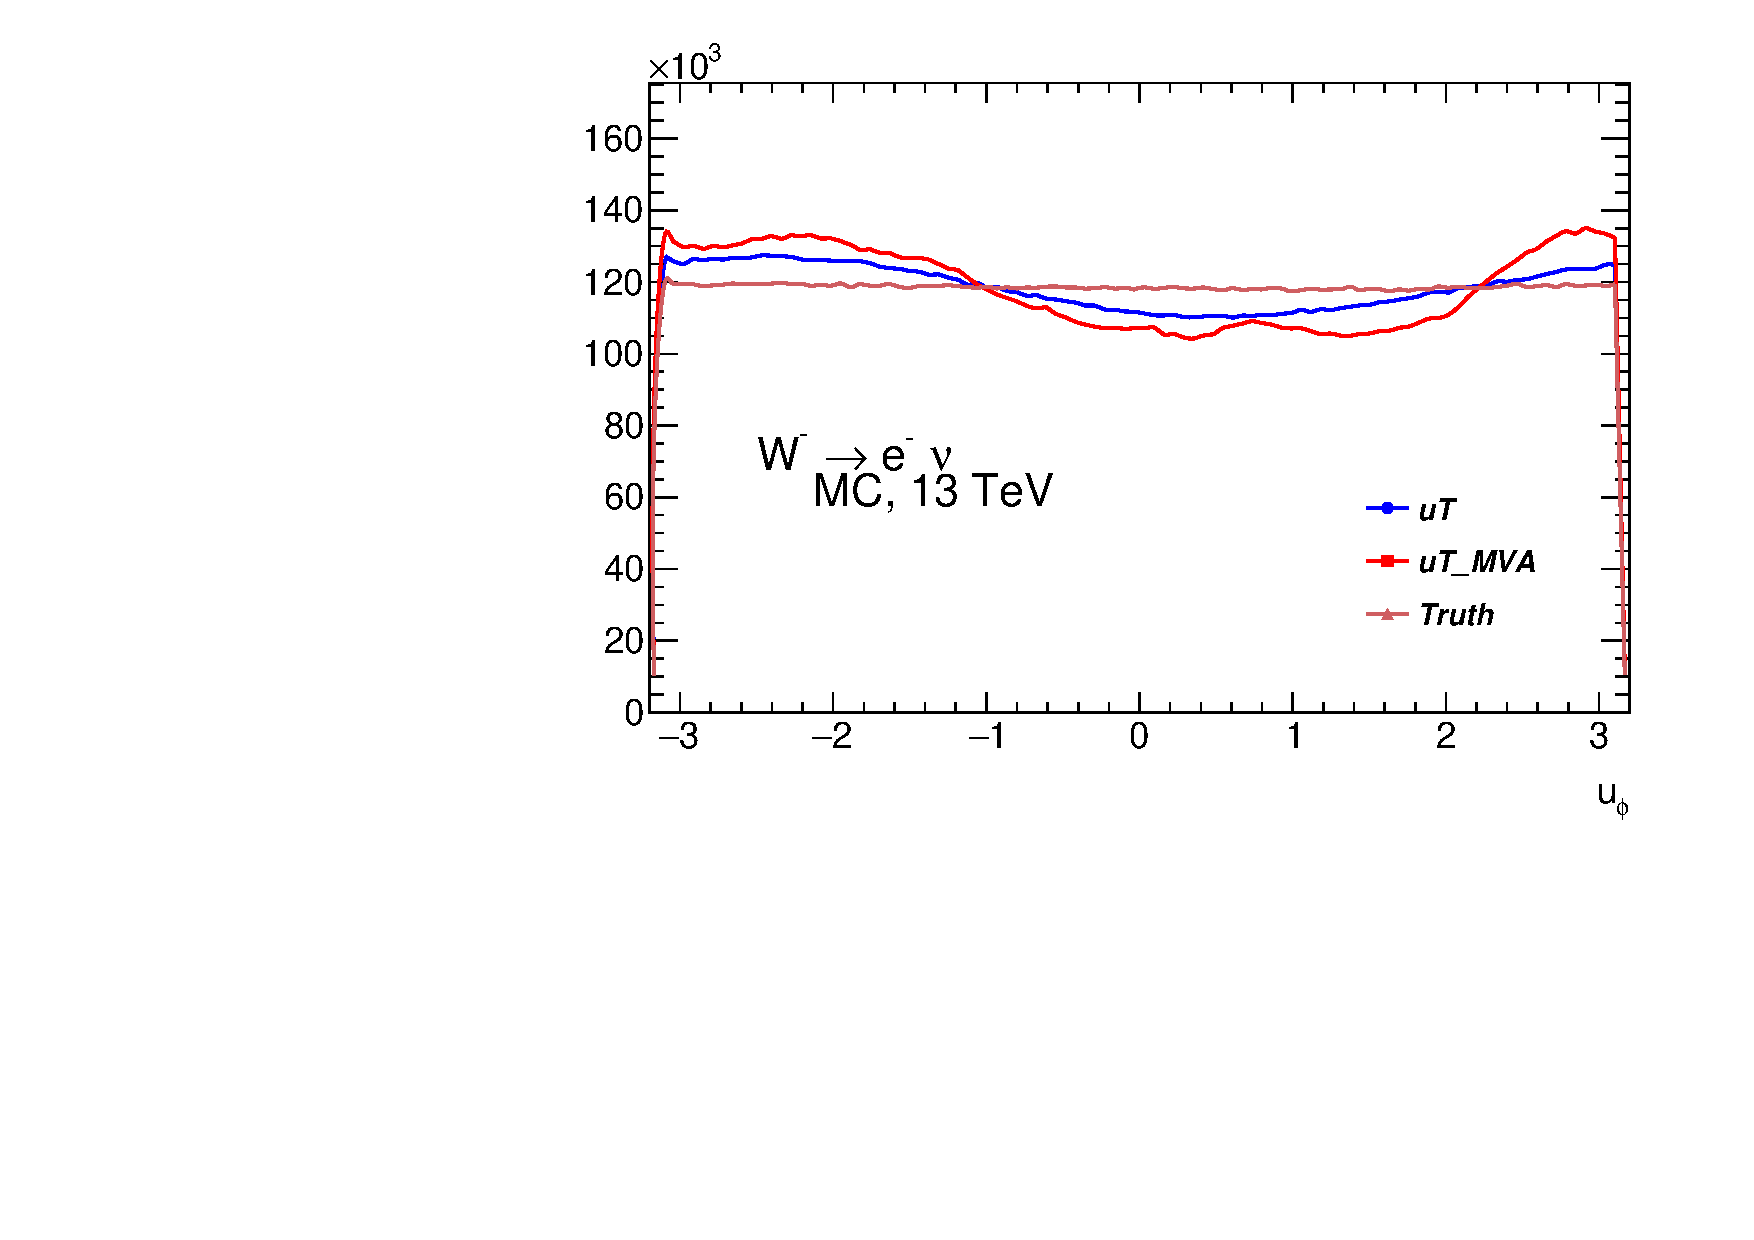
\includegraphics[width=.49\textwidth]{hist_uPhiminusenu.pdf}}\\
    	{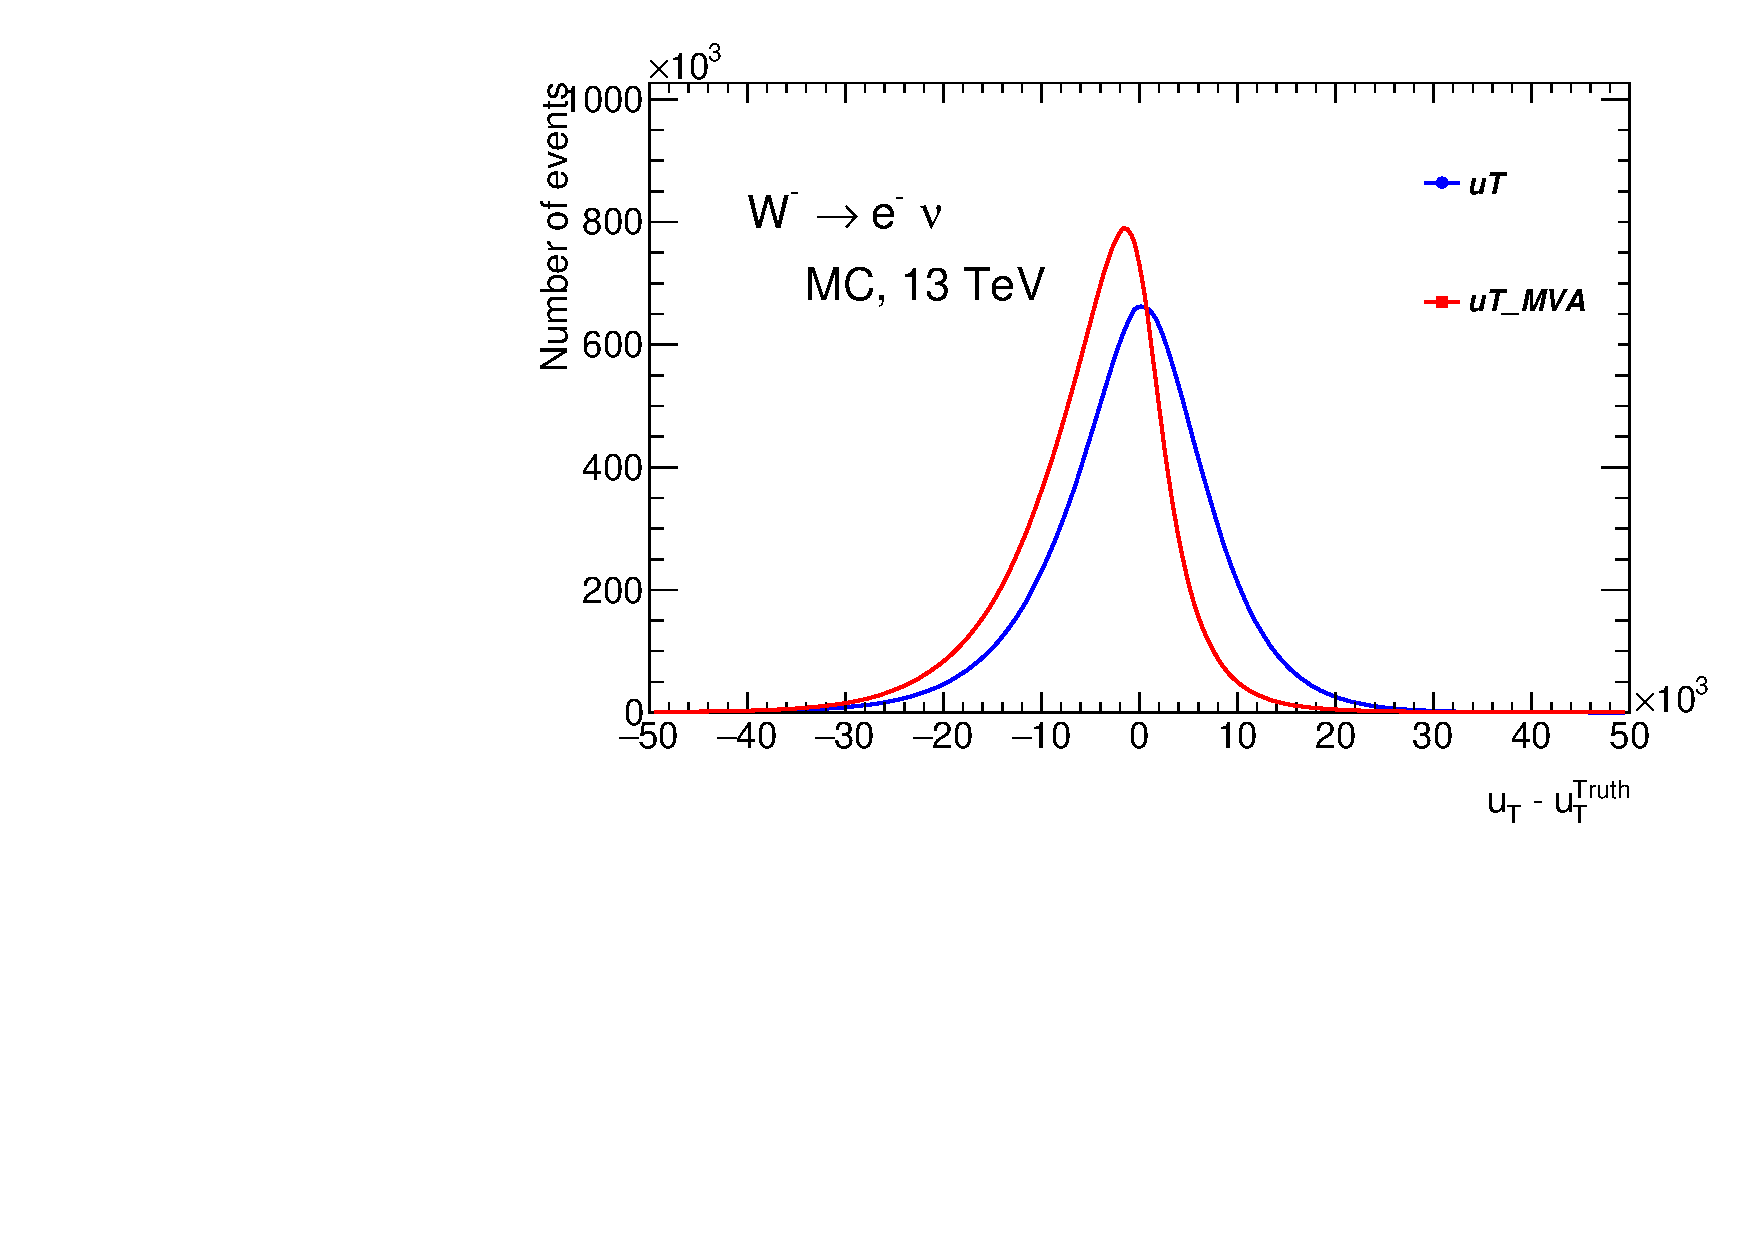
\includegraphics[width=.49\textwidth]{histosDeltaUtminusenu.pdf}}
    	{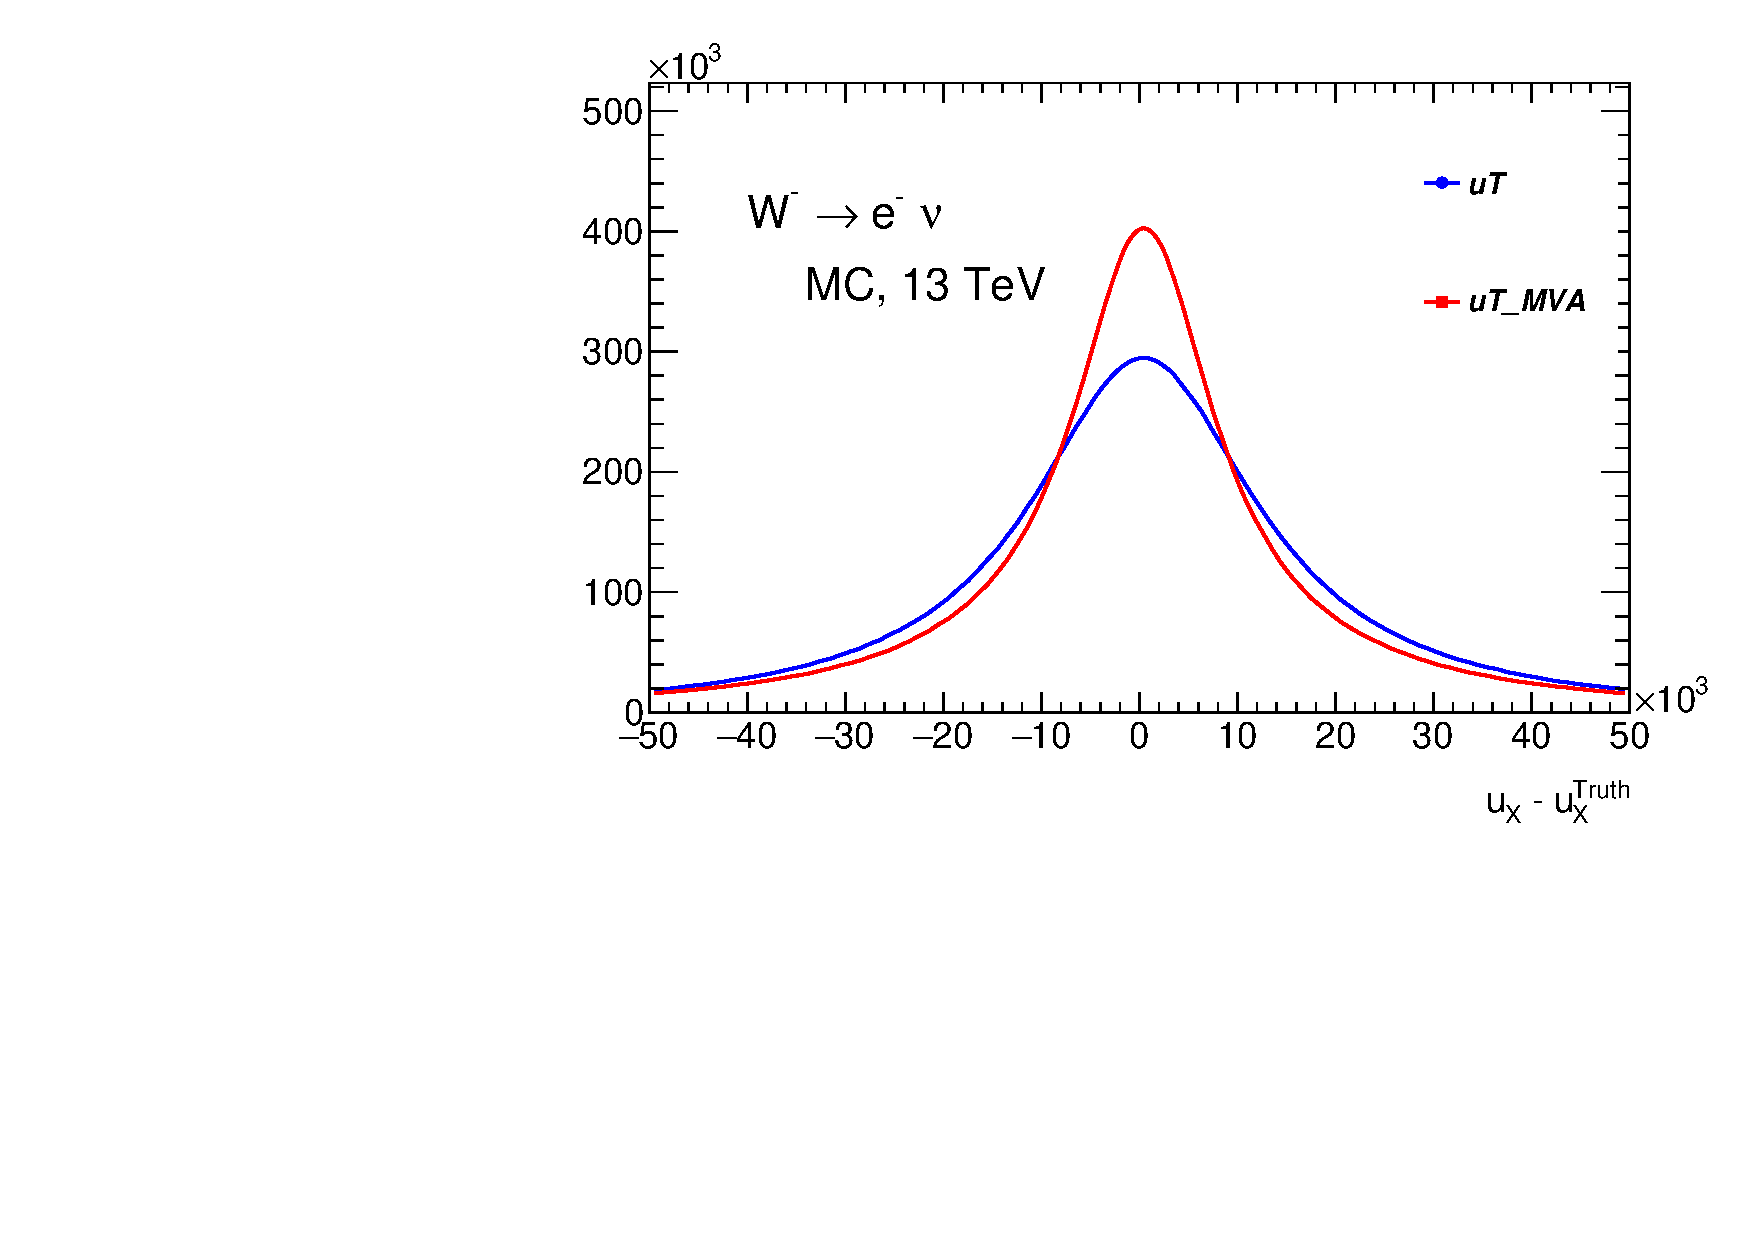
\includegraphics[width=.49\textwidth]{histosDeltaUxminusenu.pdf}} \\
    	{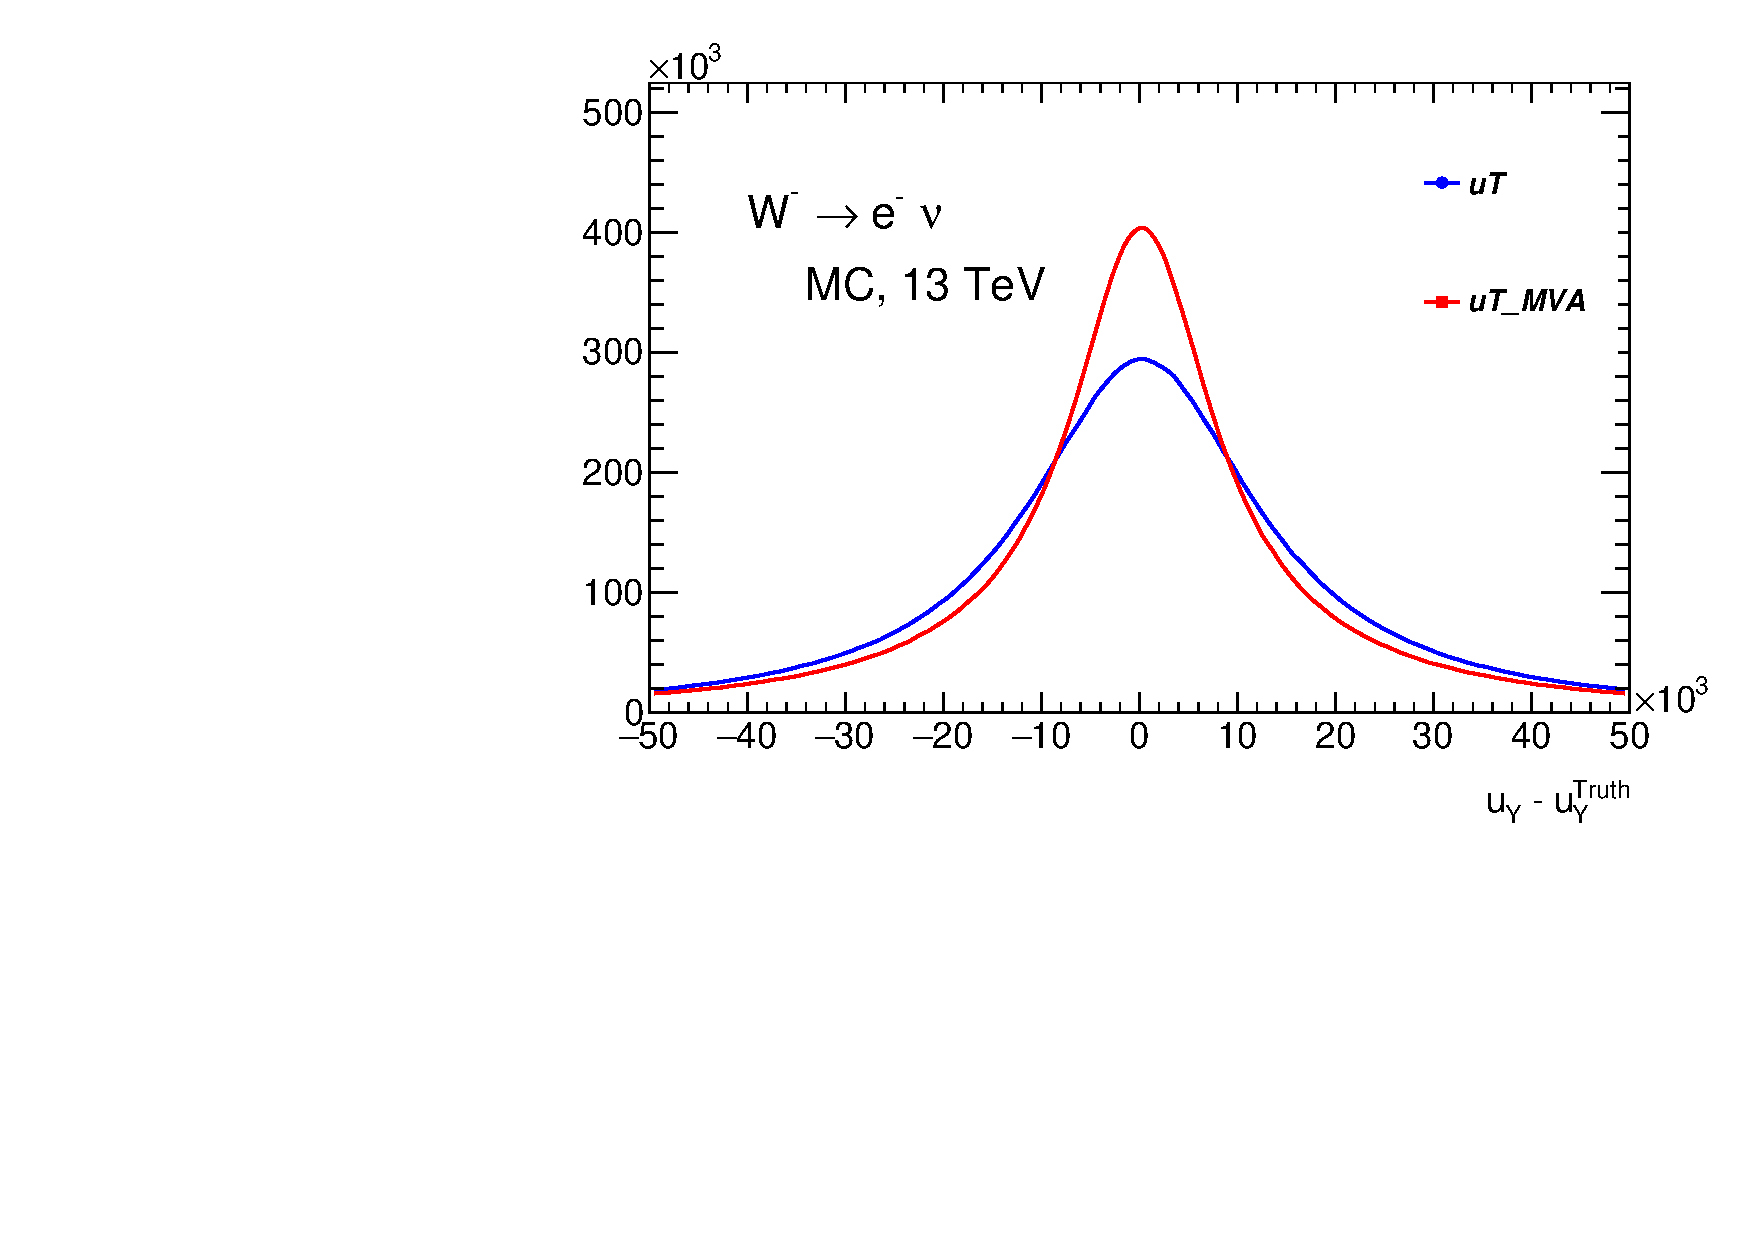
\includegraphics[width=.49\textwidth]{histosDeltaUyminusenu.pdf}}
    	{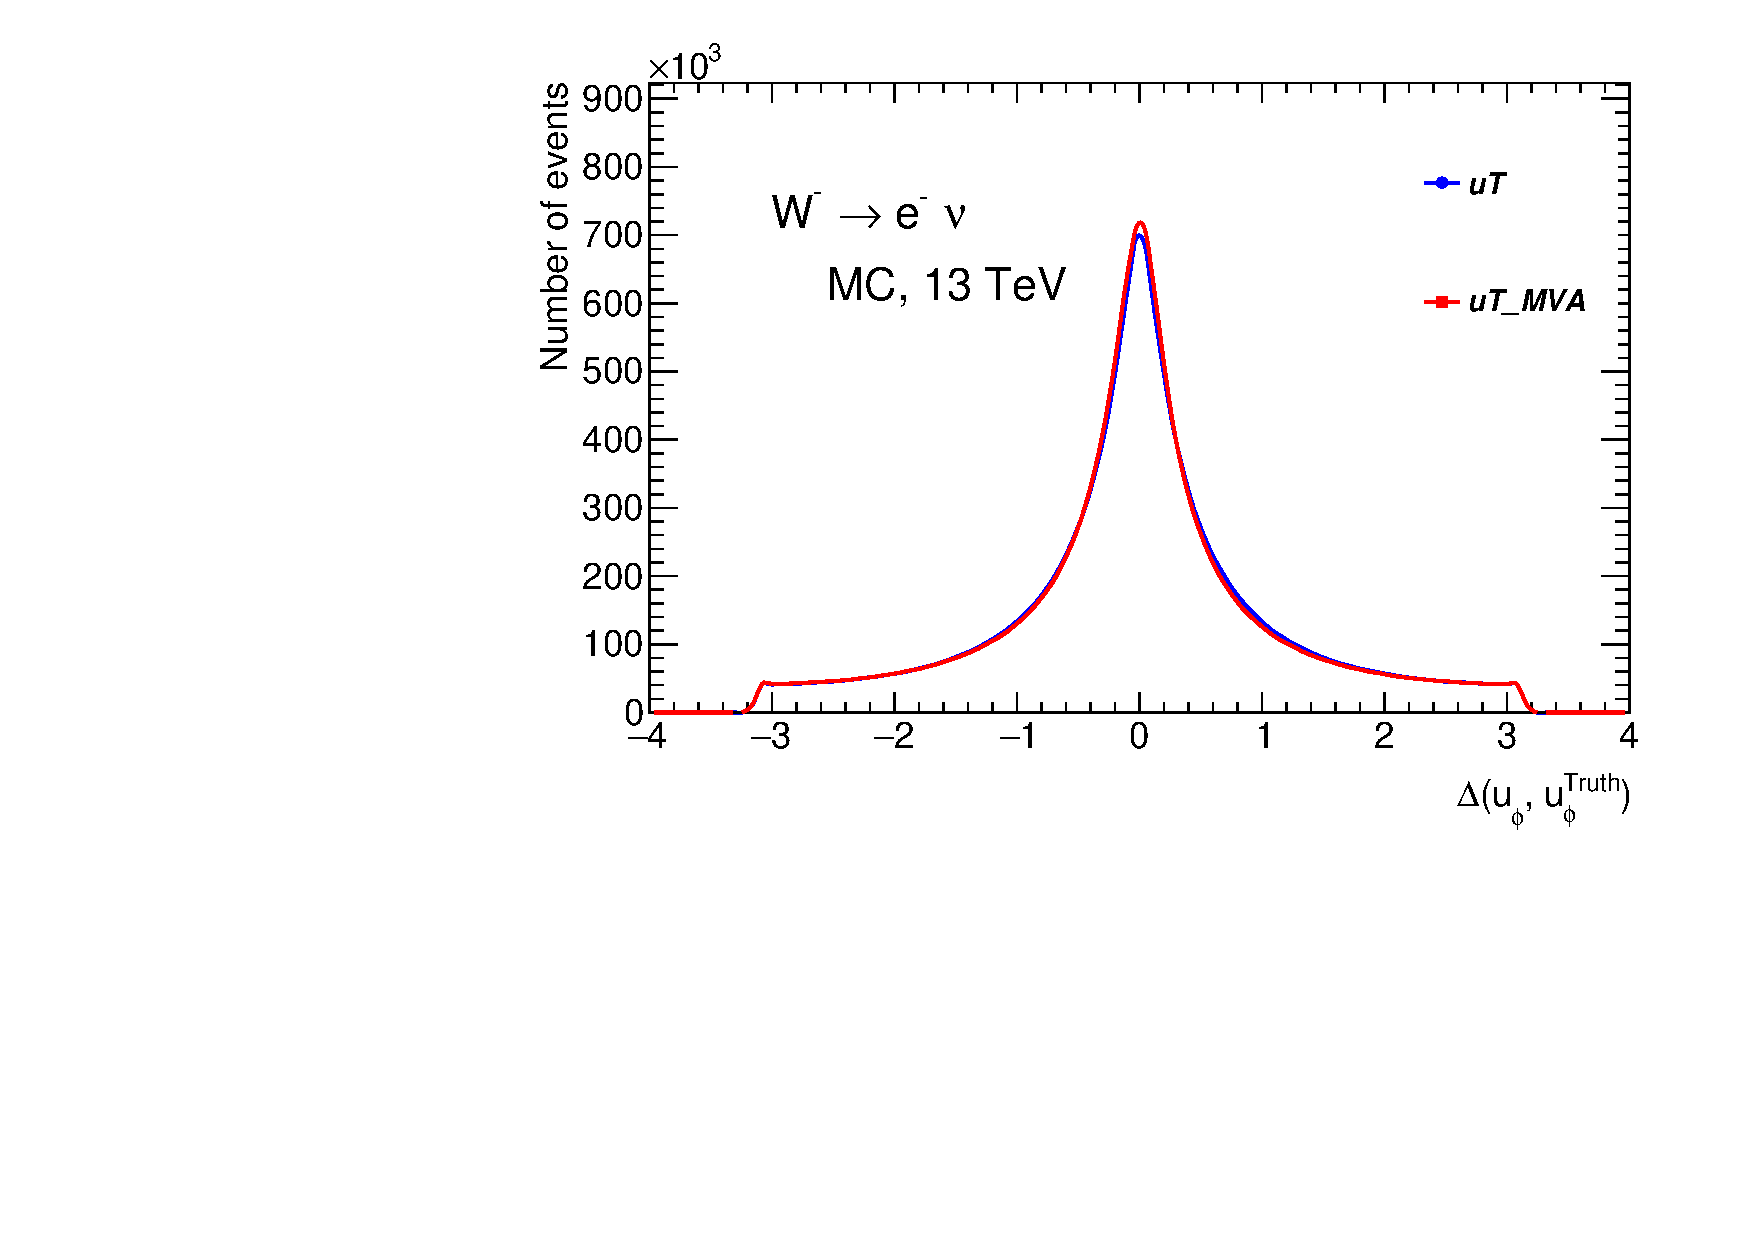
\includegraphics[width=.49\textwidth]{histosDeltaUPhiminusenu.pdf}}\\
    	\label{fig:minusenu_data_distributions1}
    \end{figure}
    \begin{figure}[h]
    	\centering
    	{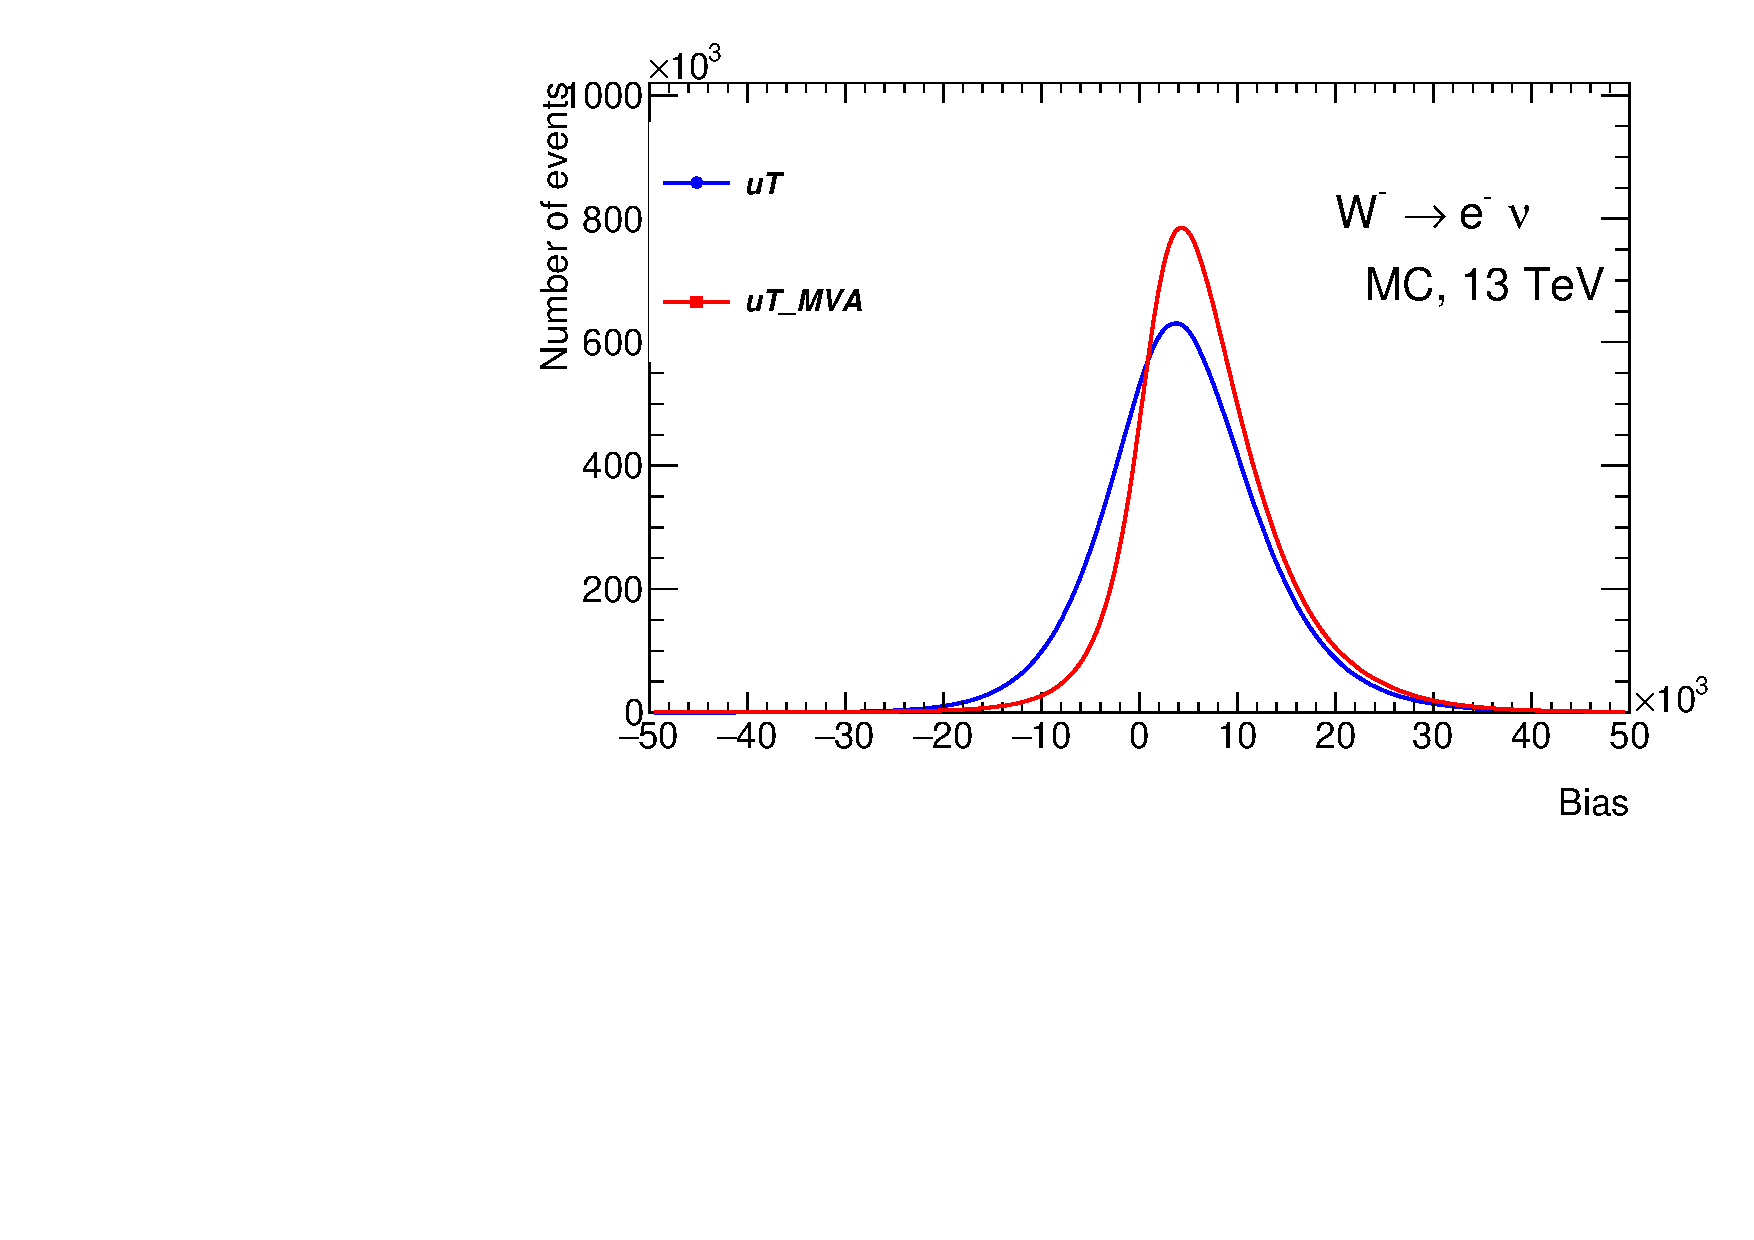
\includegraphics[width=.49\textwidth]{outMVA_biasminusenu}}
    	{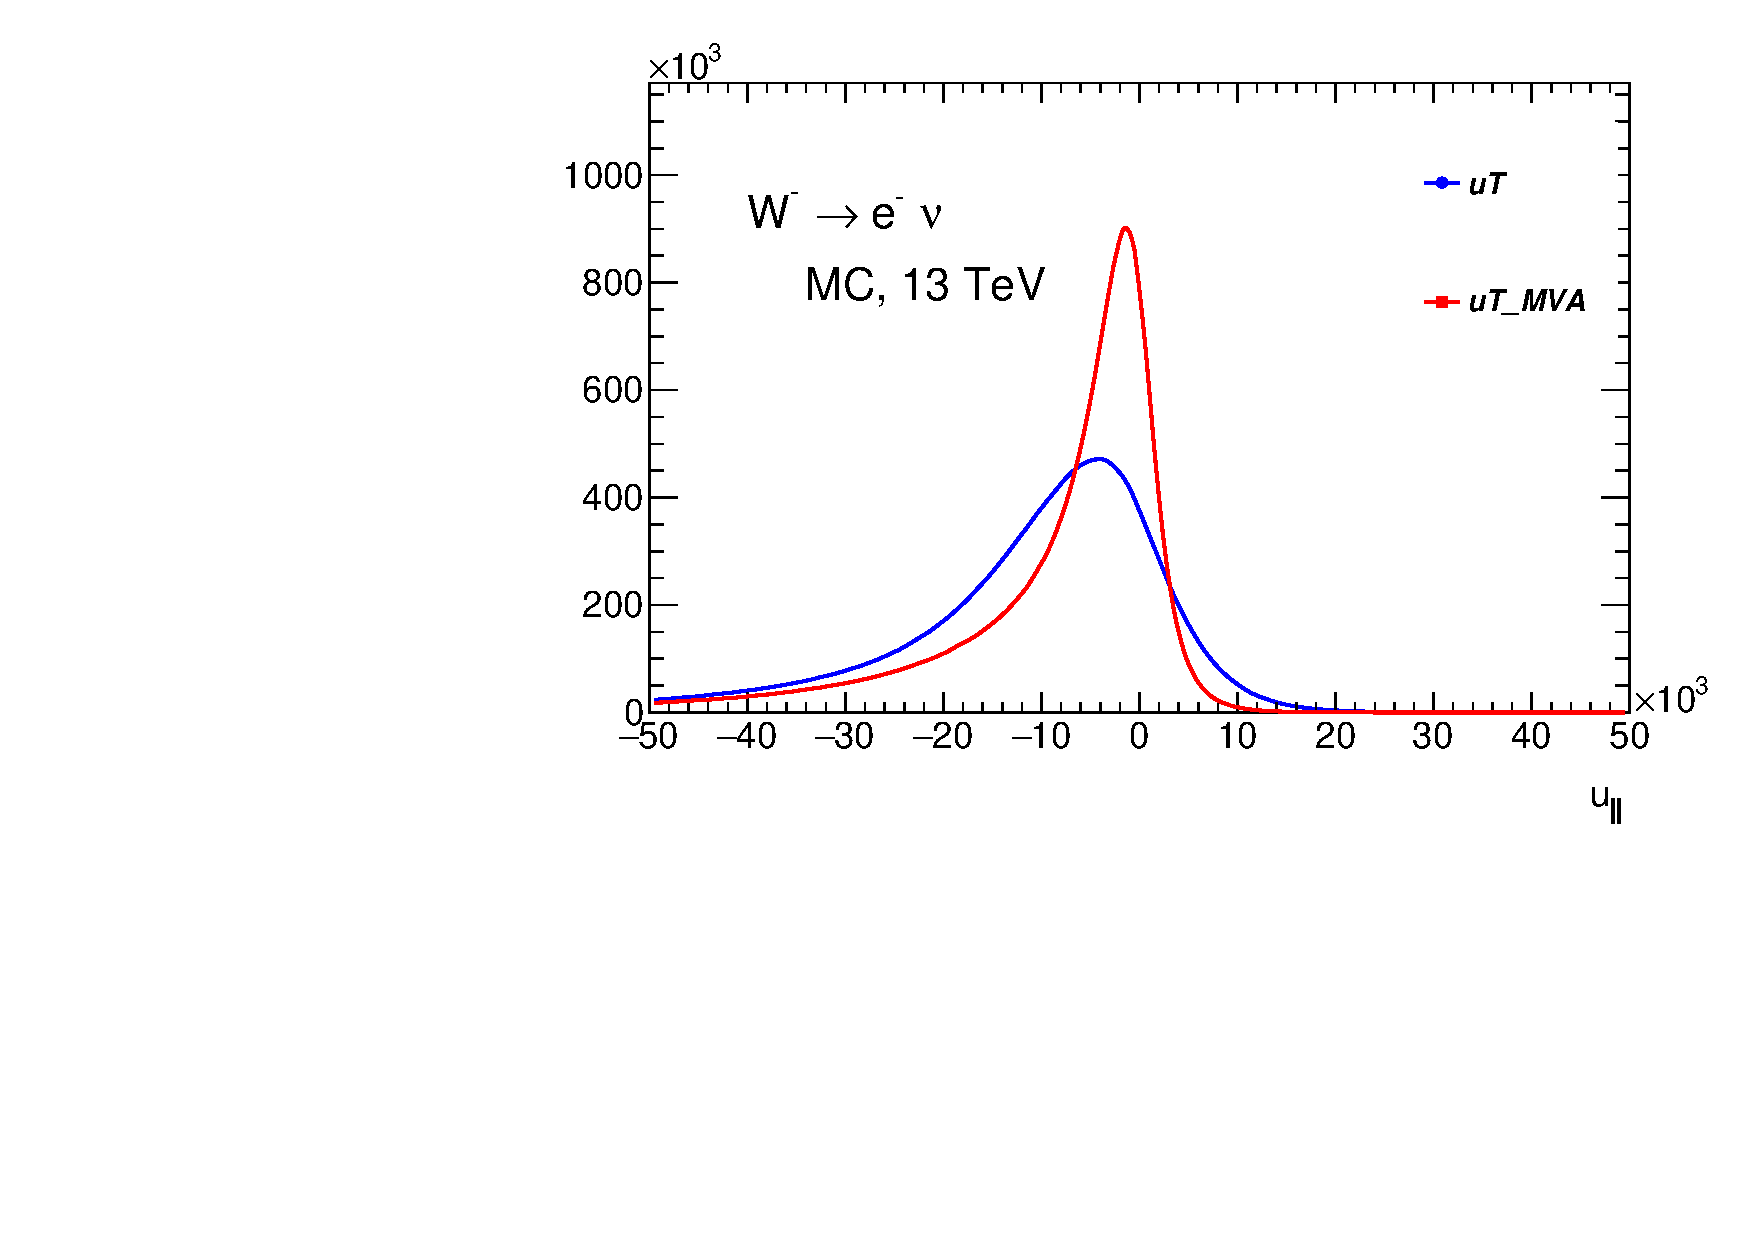
\includegraphics[width=.49\textwidth]{outMVA_Uparminusenu}}
    	{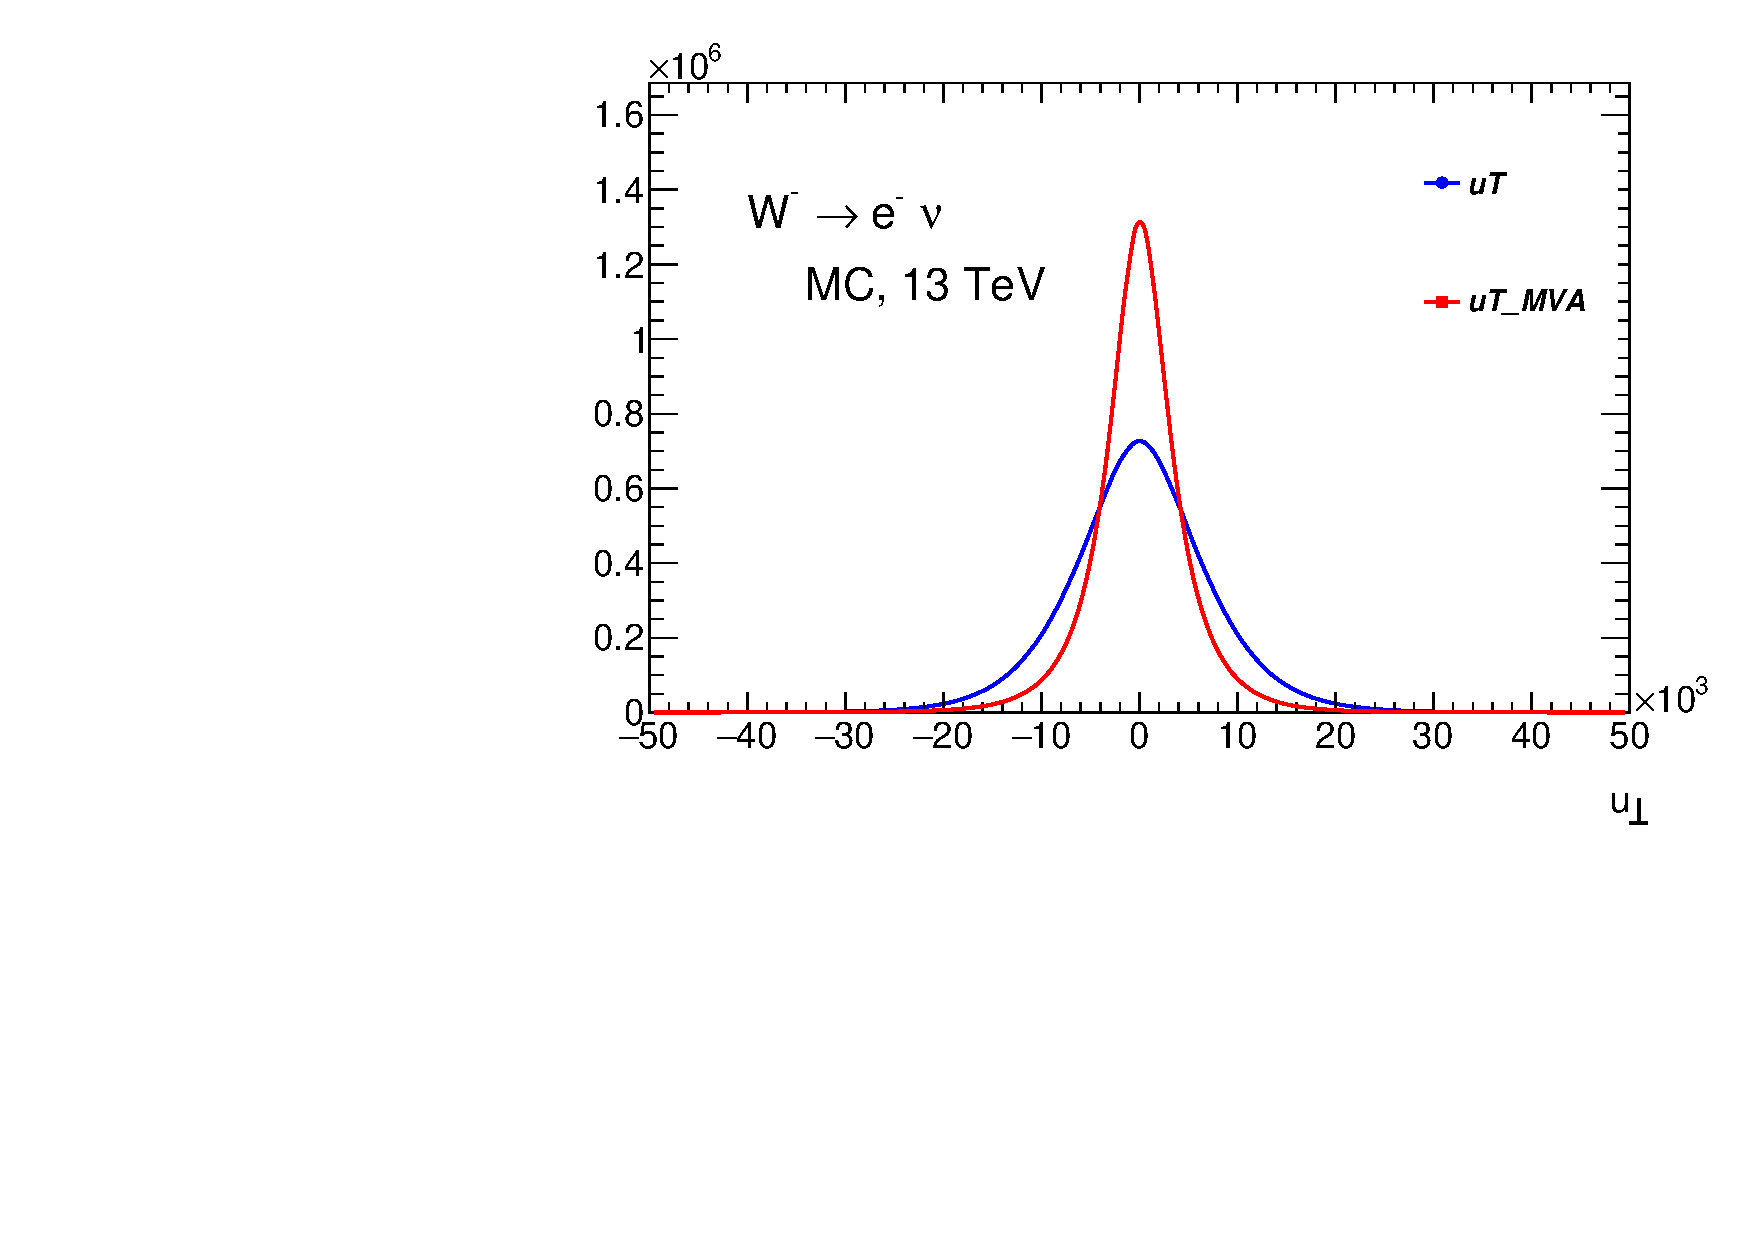
\includegraphics[width=.49\textwidth]{outMVA_uPerpminusenu}}
    	{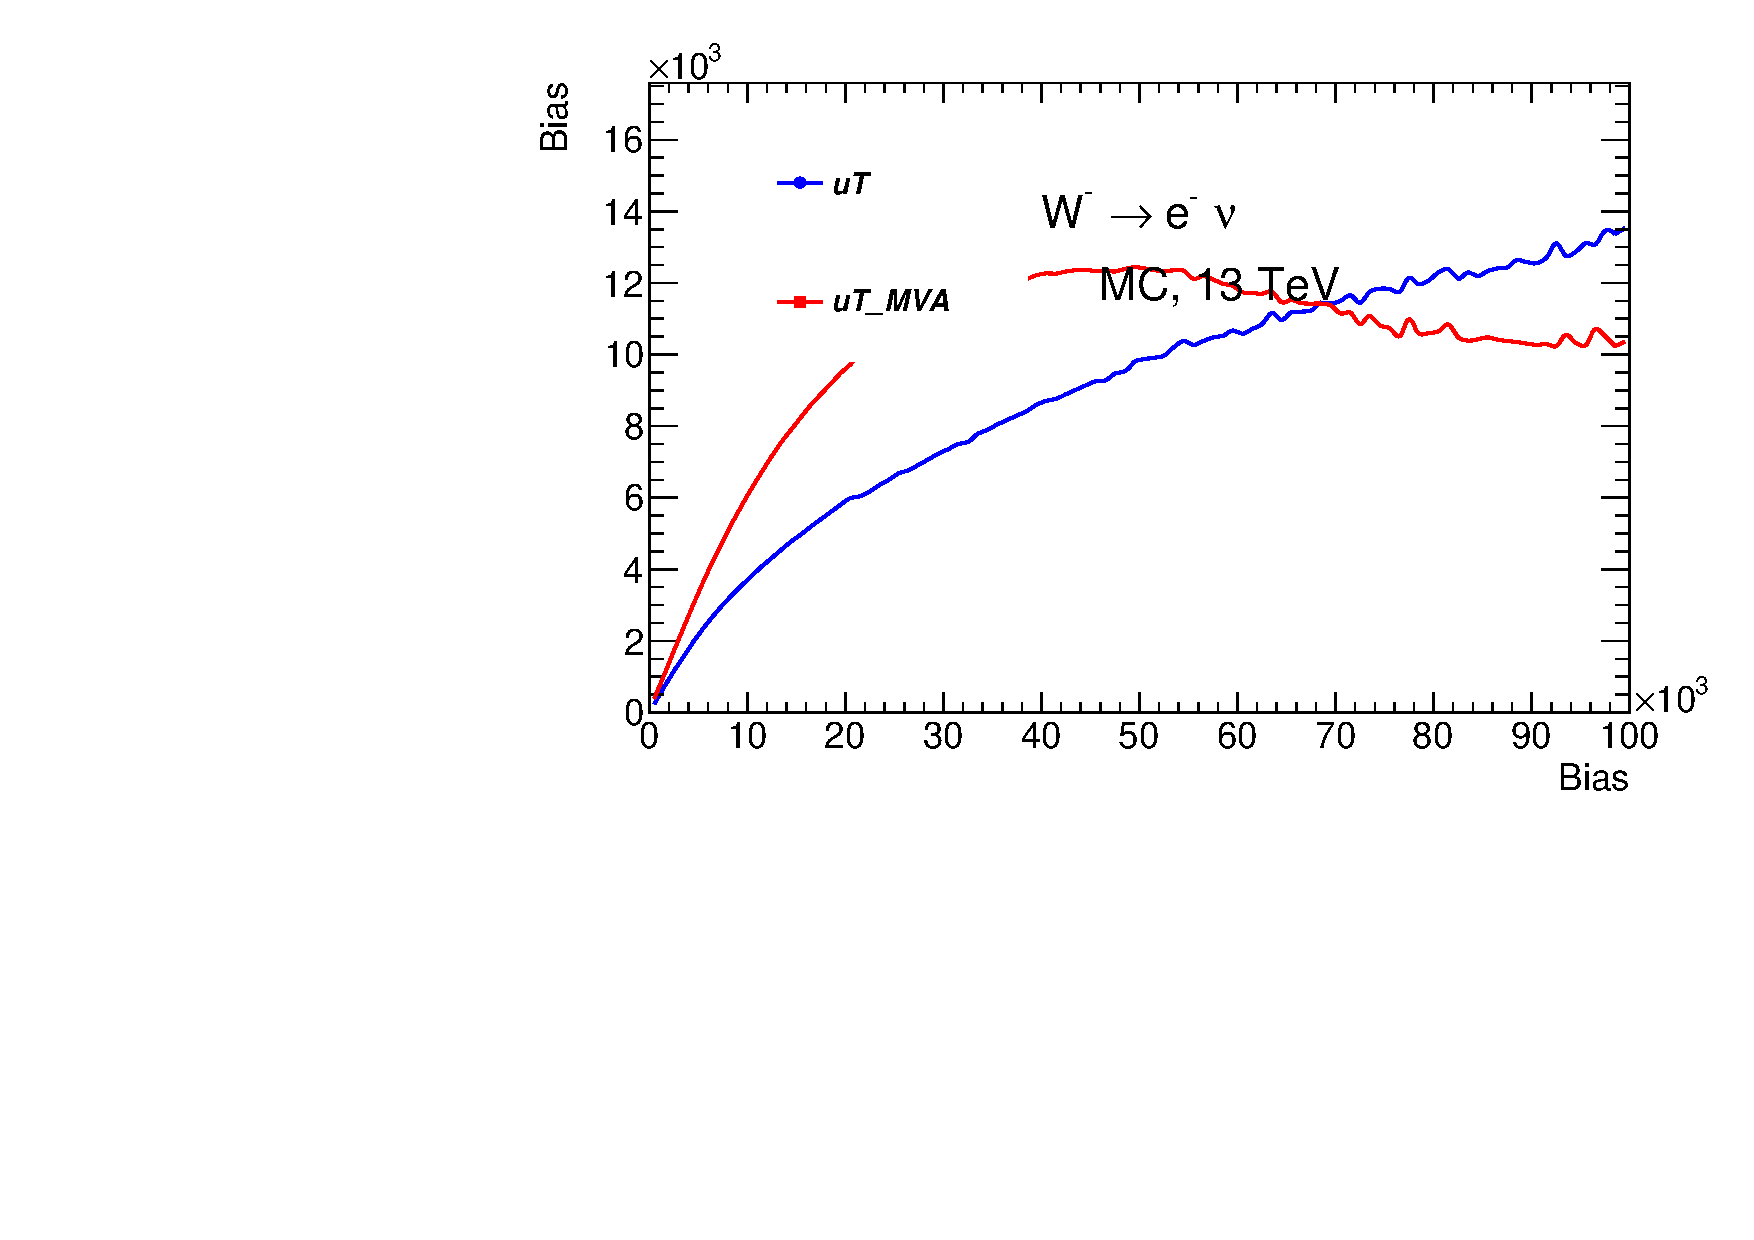
\includegraphics[width=.49\textwidth]{histosMeanBiasminusenu}}
    	{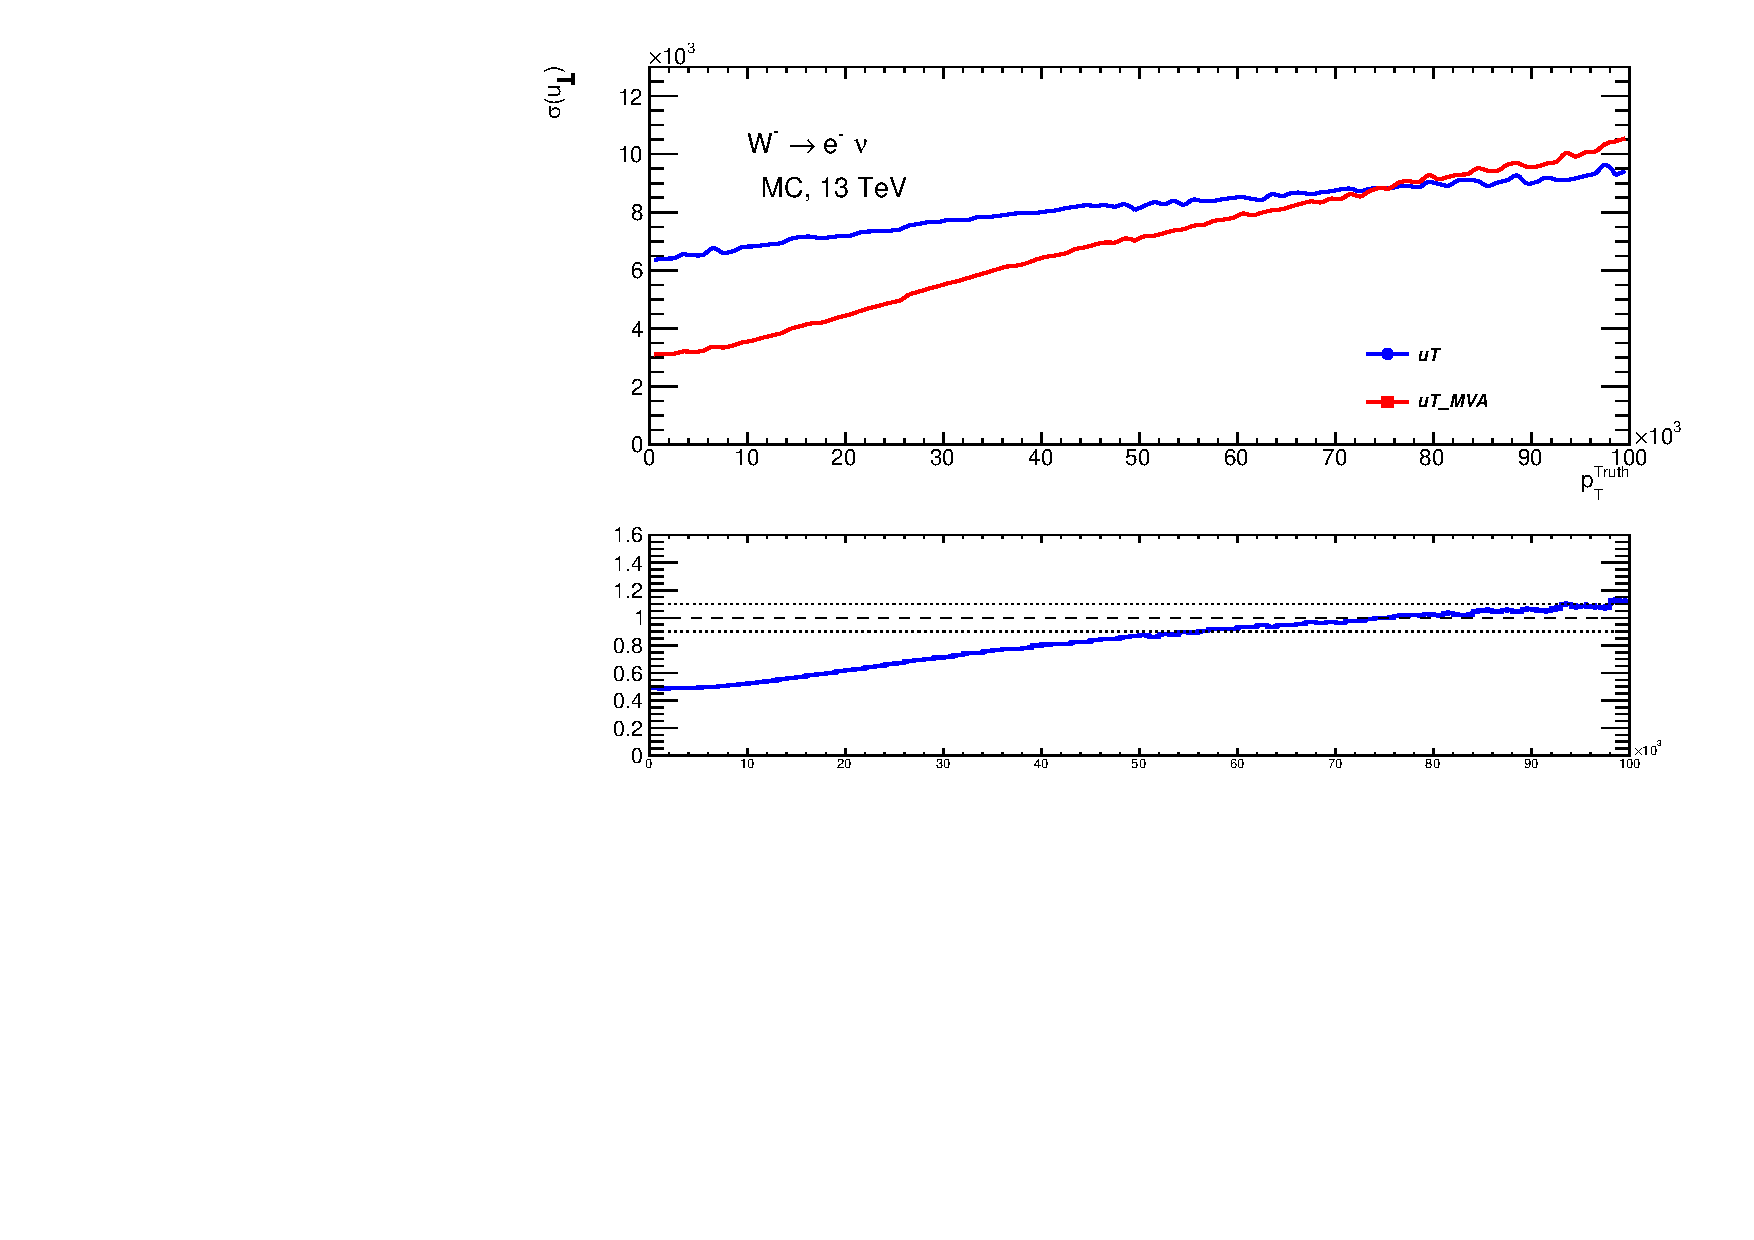
\includegraphics[width=.49\textwidth]{histosSigmaUperpminusenu}}
    	{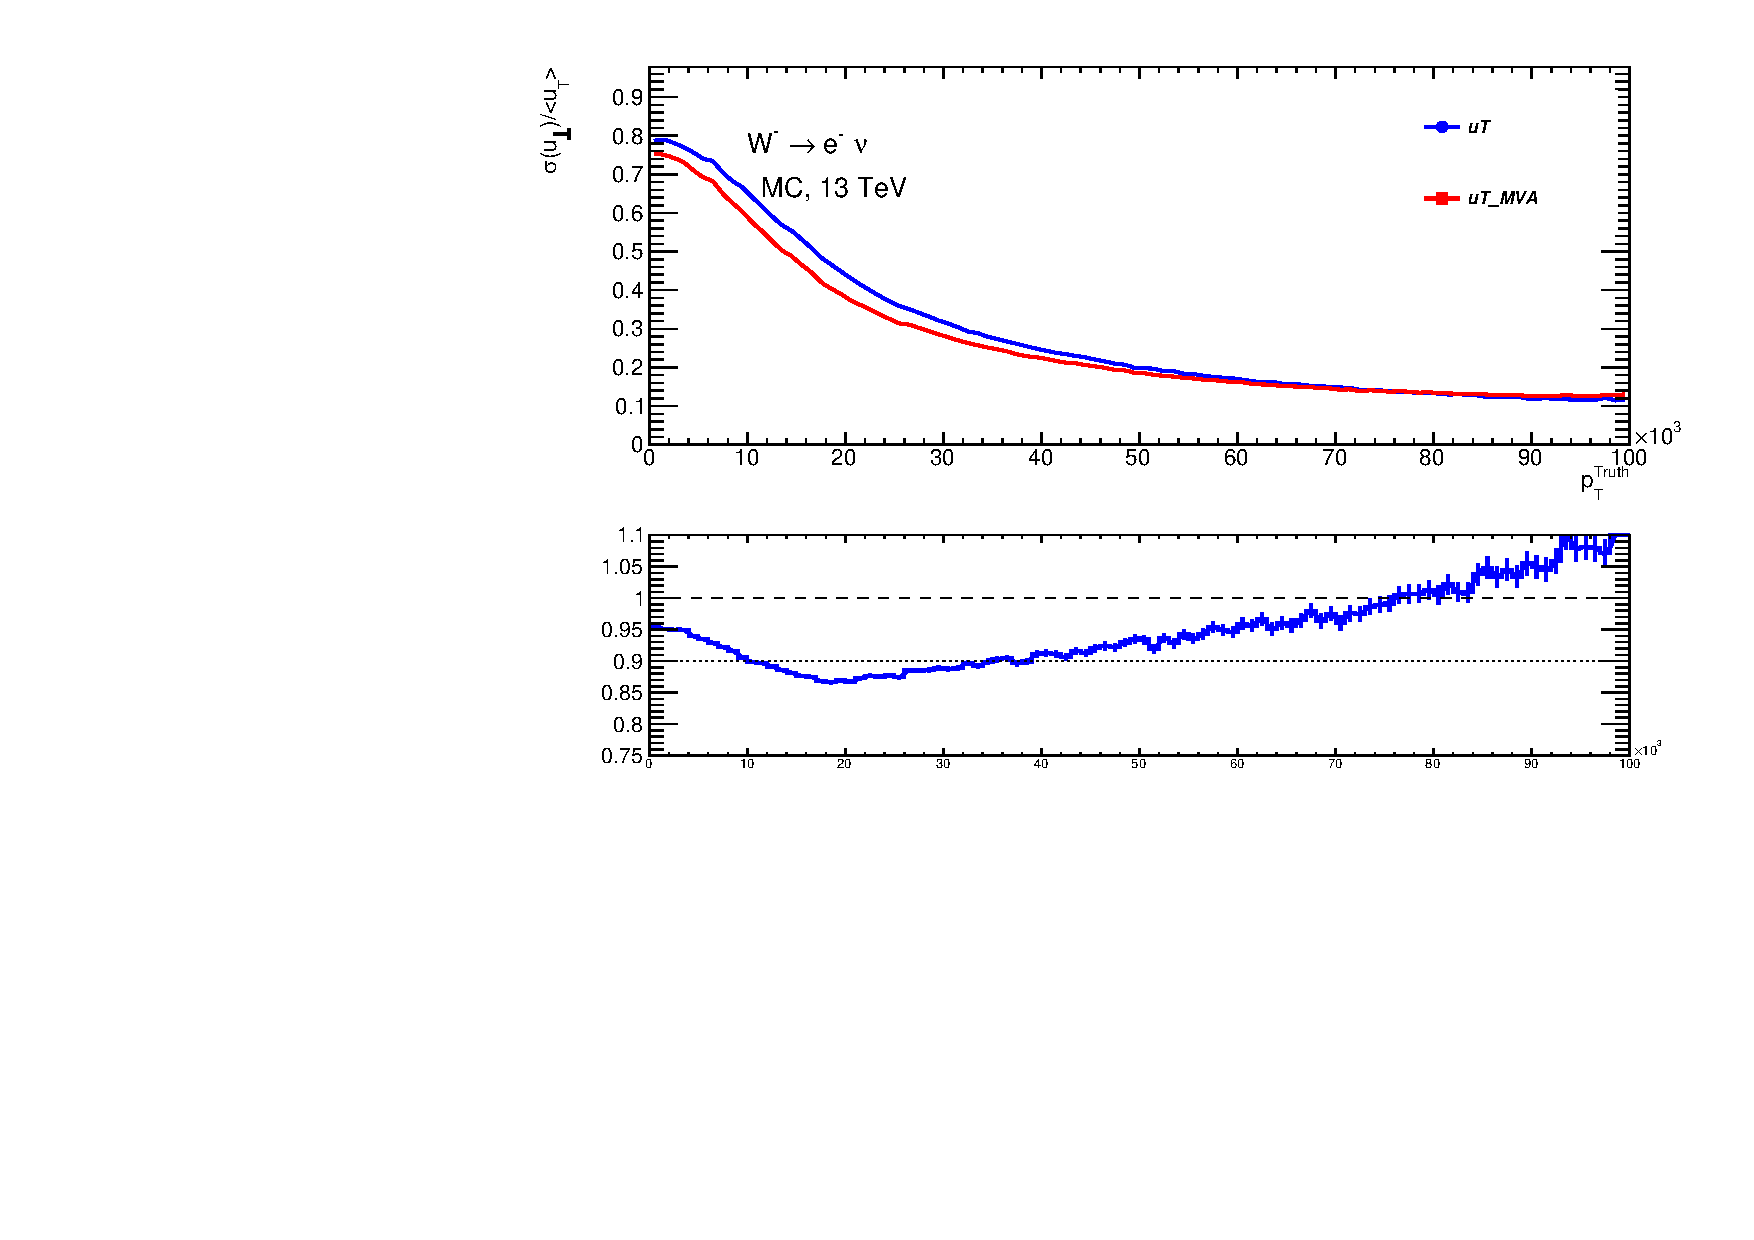
\includegraphics[width=.49\textwidth]{histosUperpRelativeminusenu}}
    	\caption{Comparison of kinematic distributions of $u_T$ vs $u_T^{MVA}$ for $W^+\rightarrow \mu^+\nu$ data sample.}
    	\label{fig:minusenu_data_distributions2}
    \end{figure}
    
    \begin{figure}[h]
    	\centering
    	{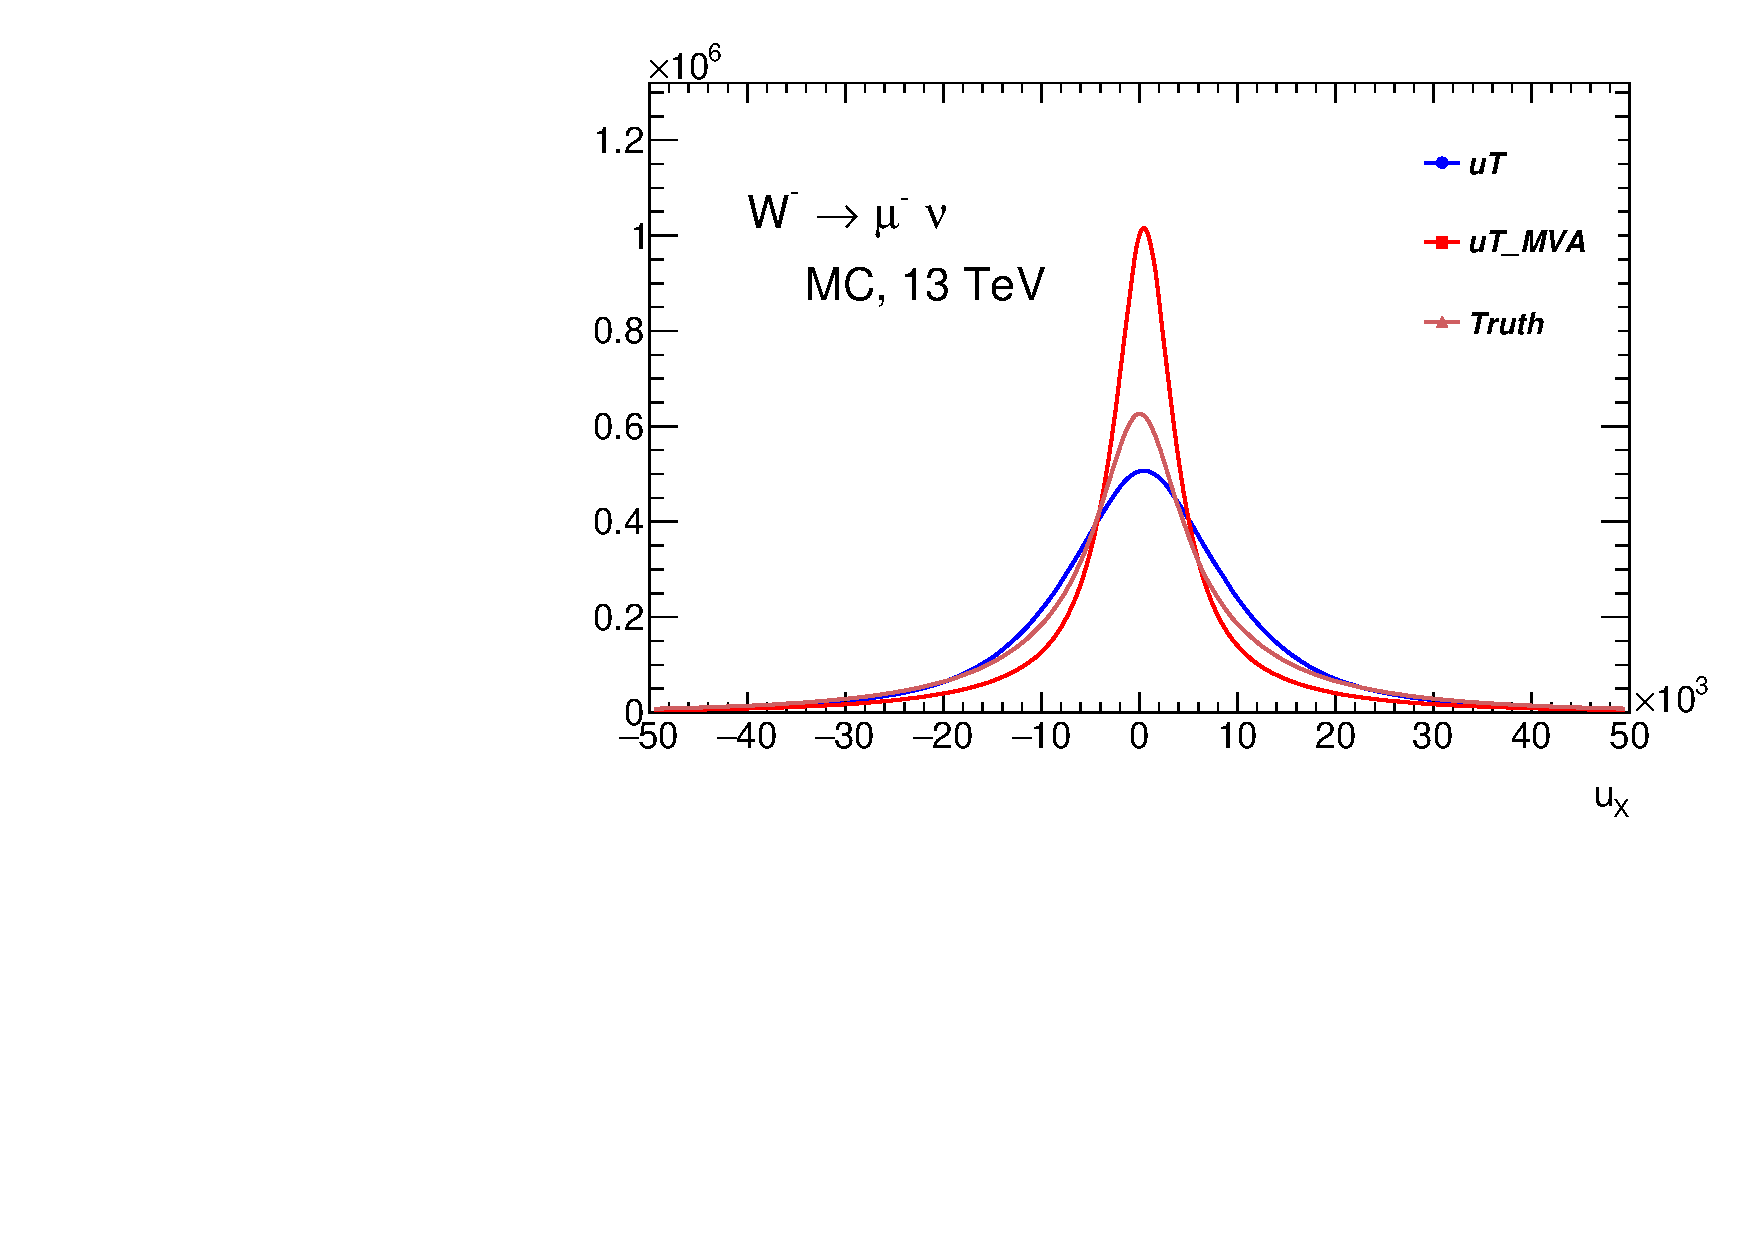
\includegraphics[width=.49\textwidth]{hist_uXminusmunu.pdf}}
    	{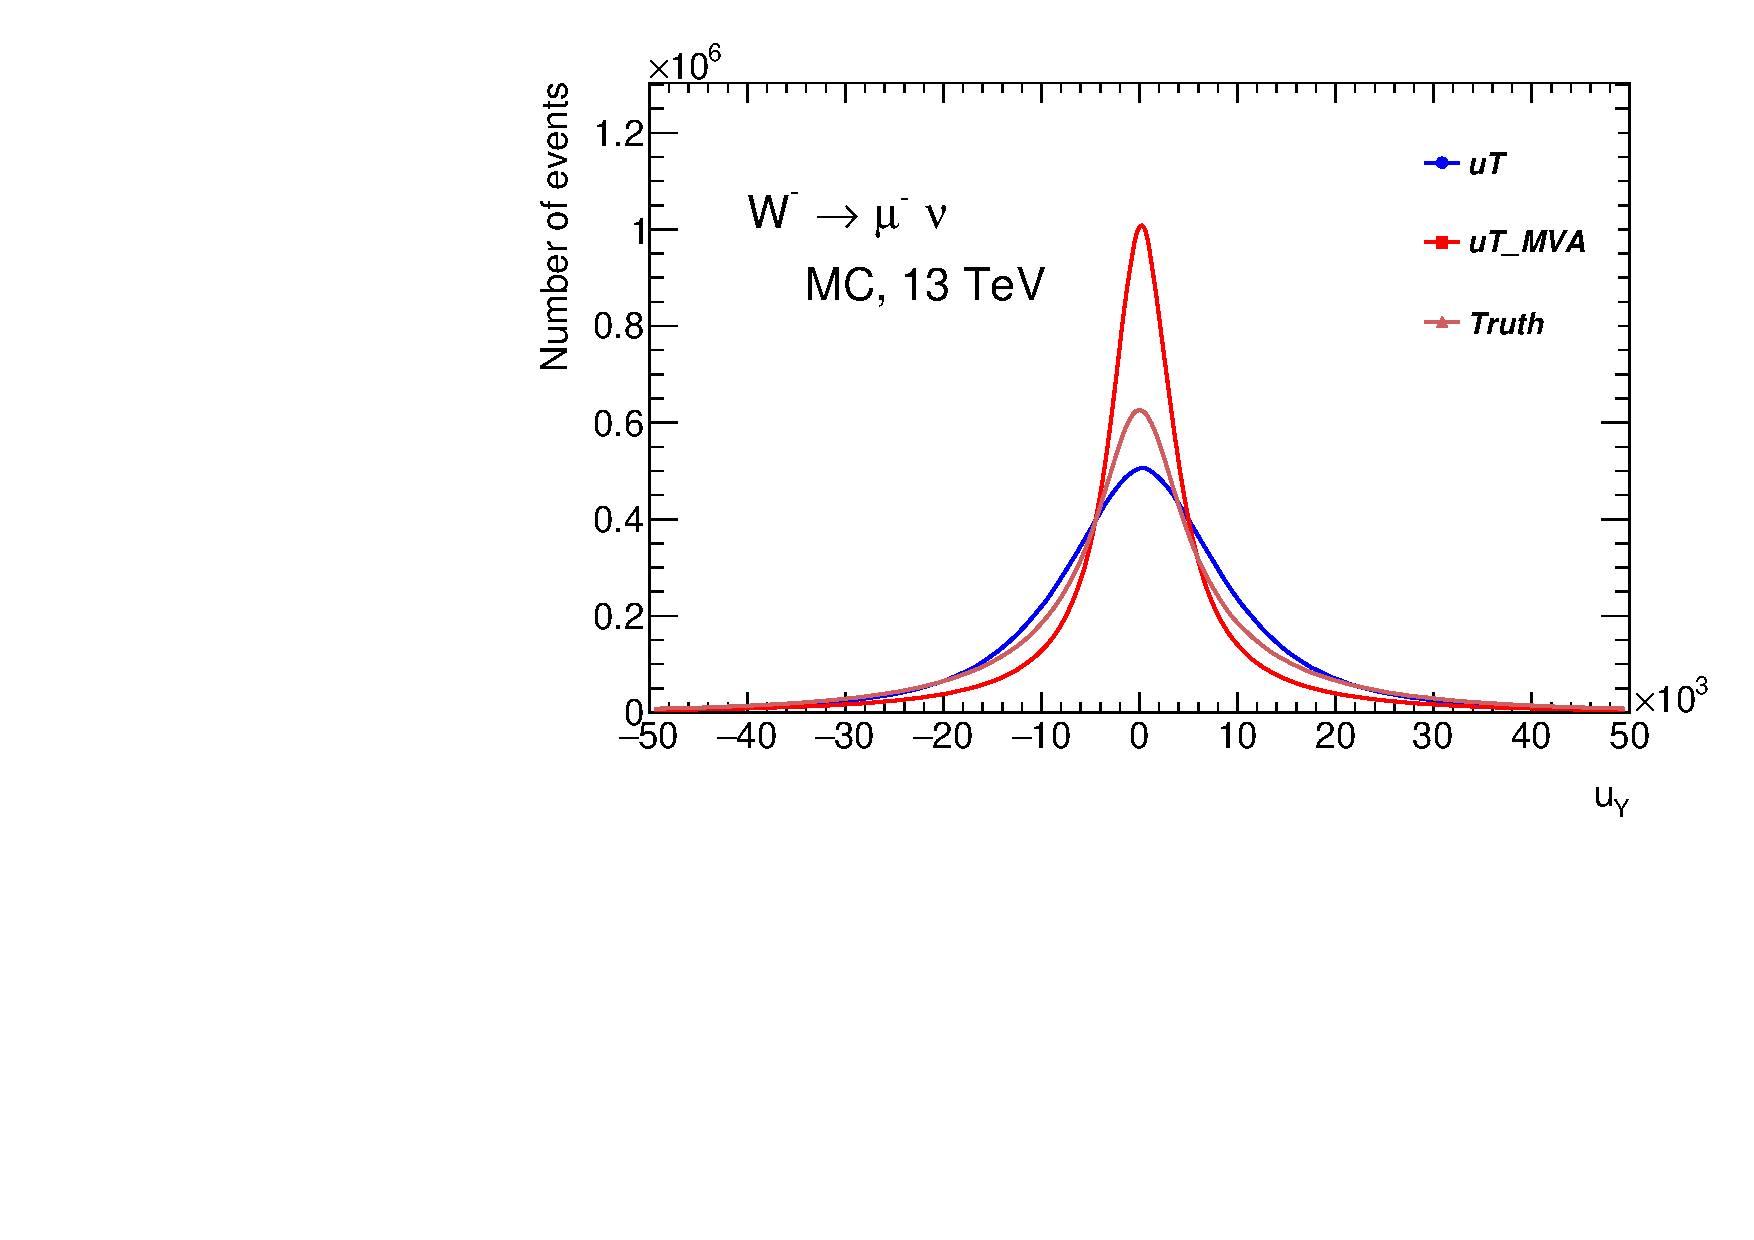
\includegraphics[width=.49\textwidth]{hist_uYminusmunu.pdf}} \\
    	{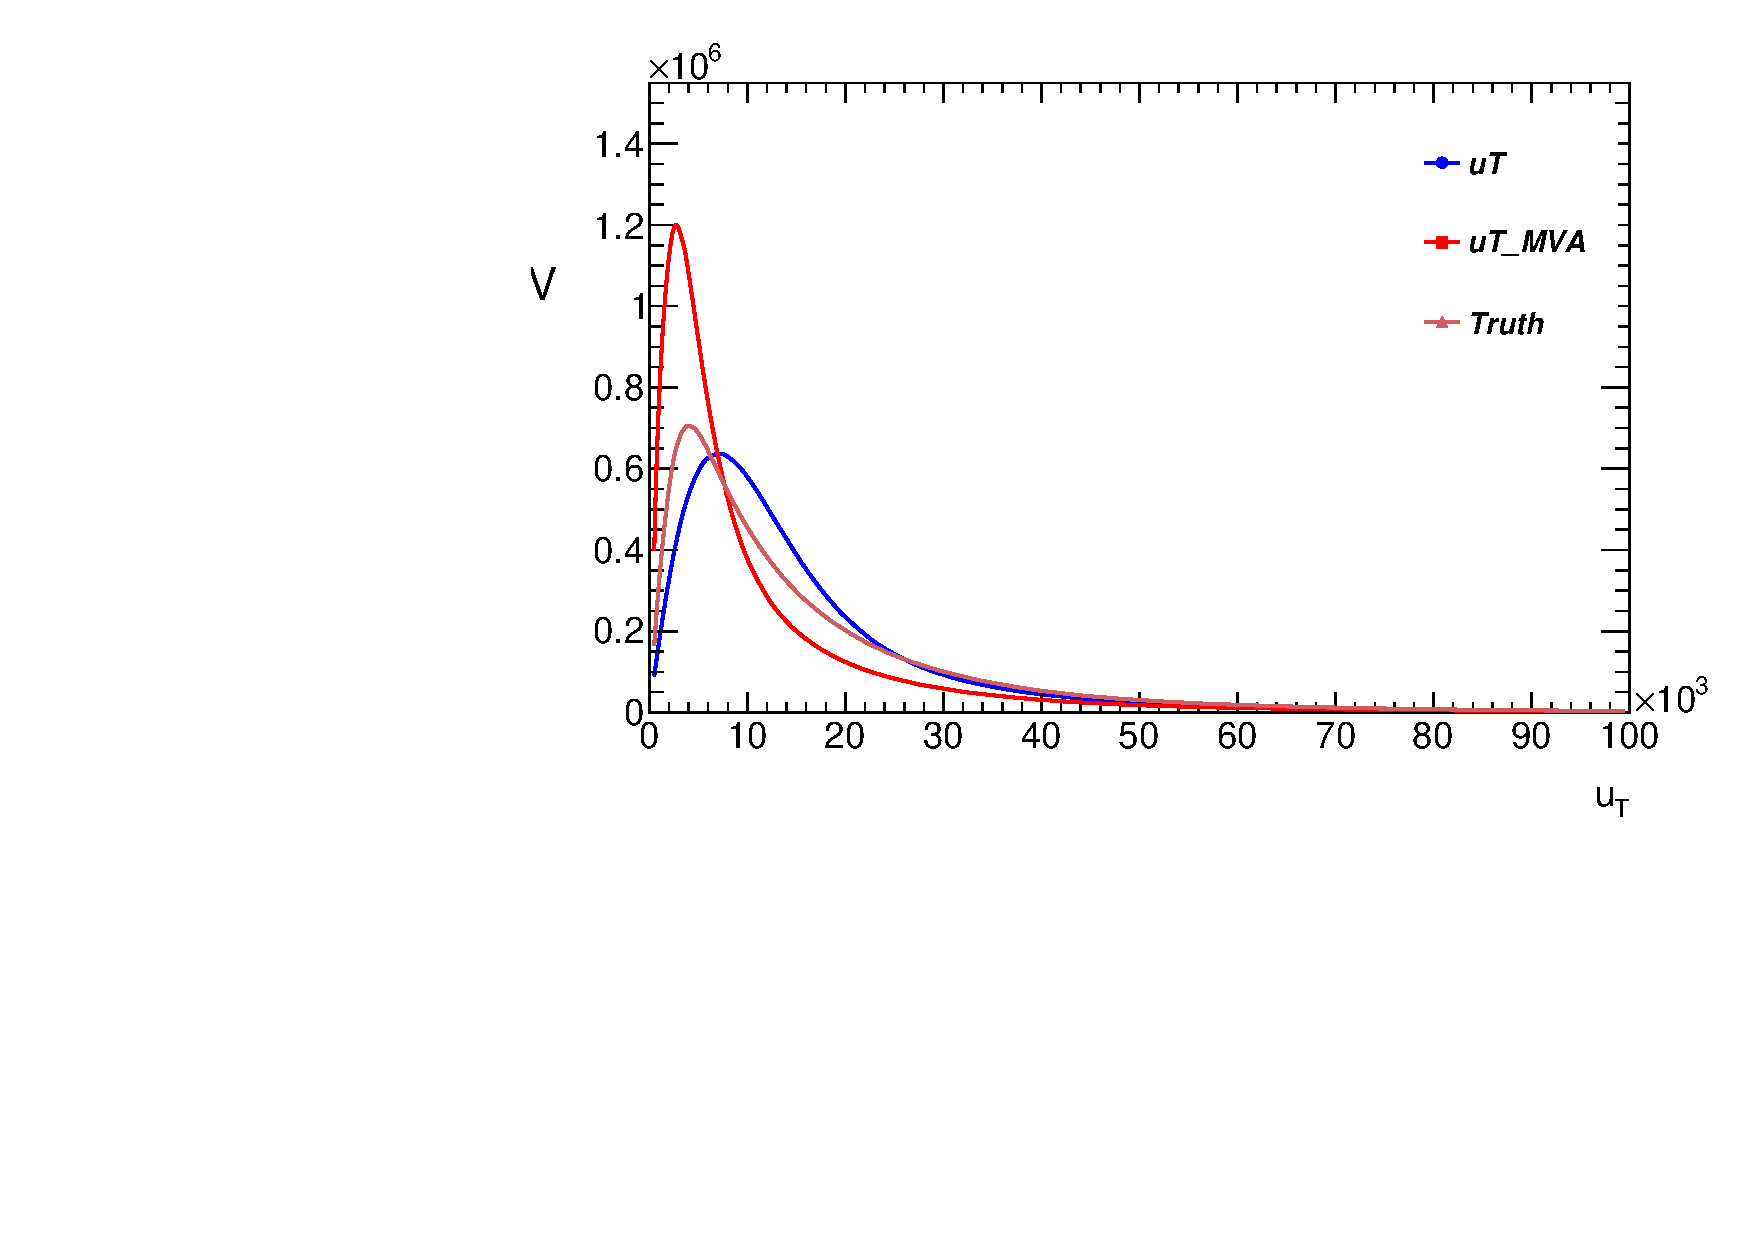
\includegraphics[width=.49\textwidth]{hist_uTminusmunu.pdf}}
    	{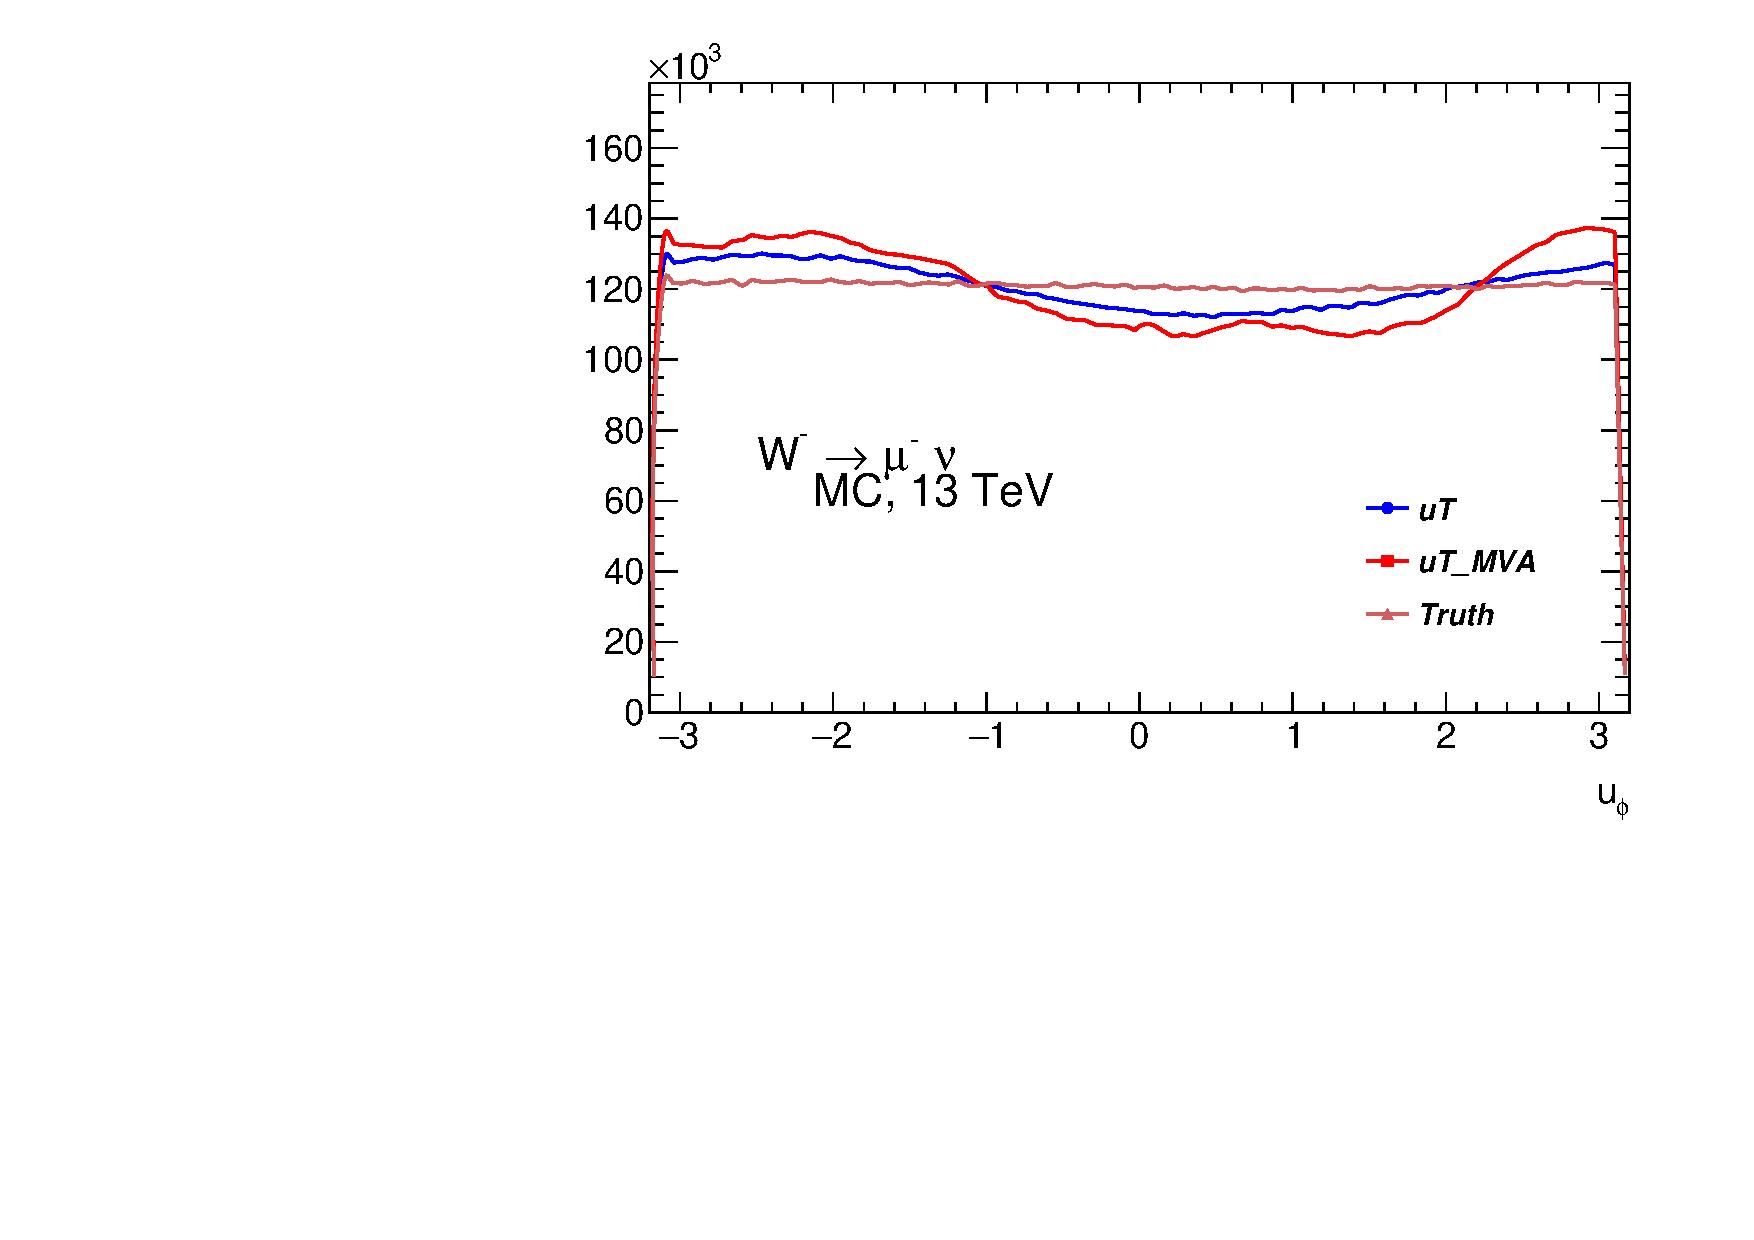
\includegraphics[width=.49\textwidth]{hist_uPhiminusmunu.pdf}}\\
    	{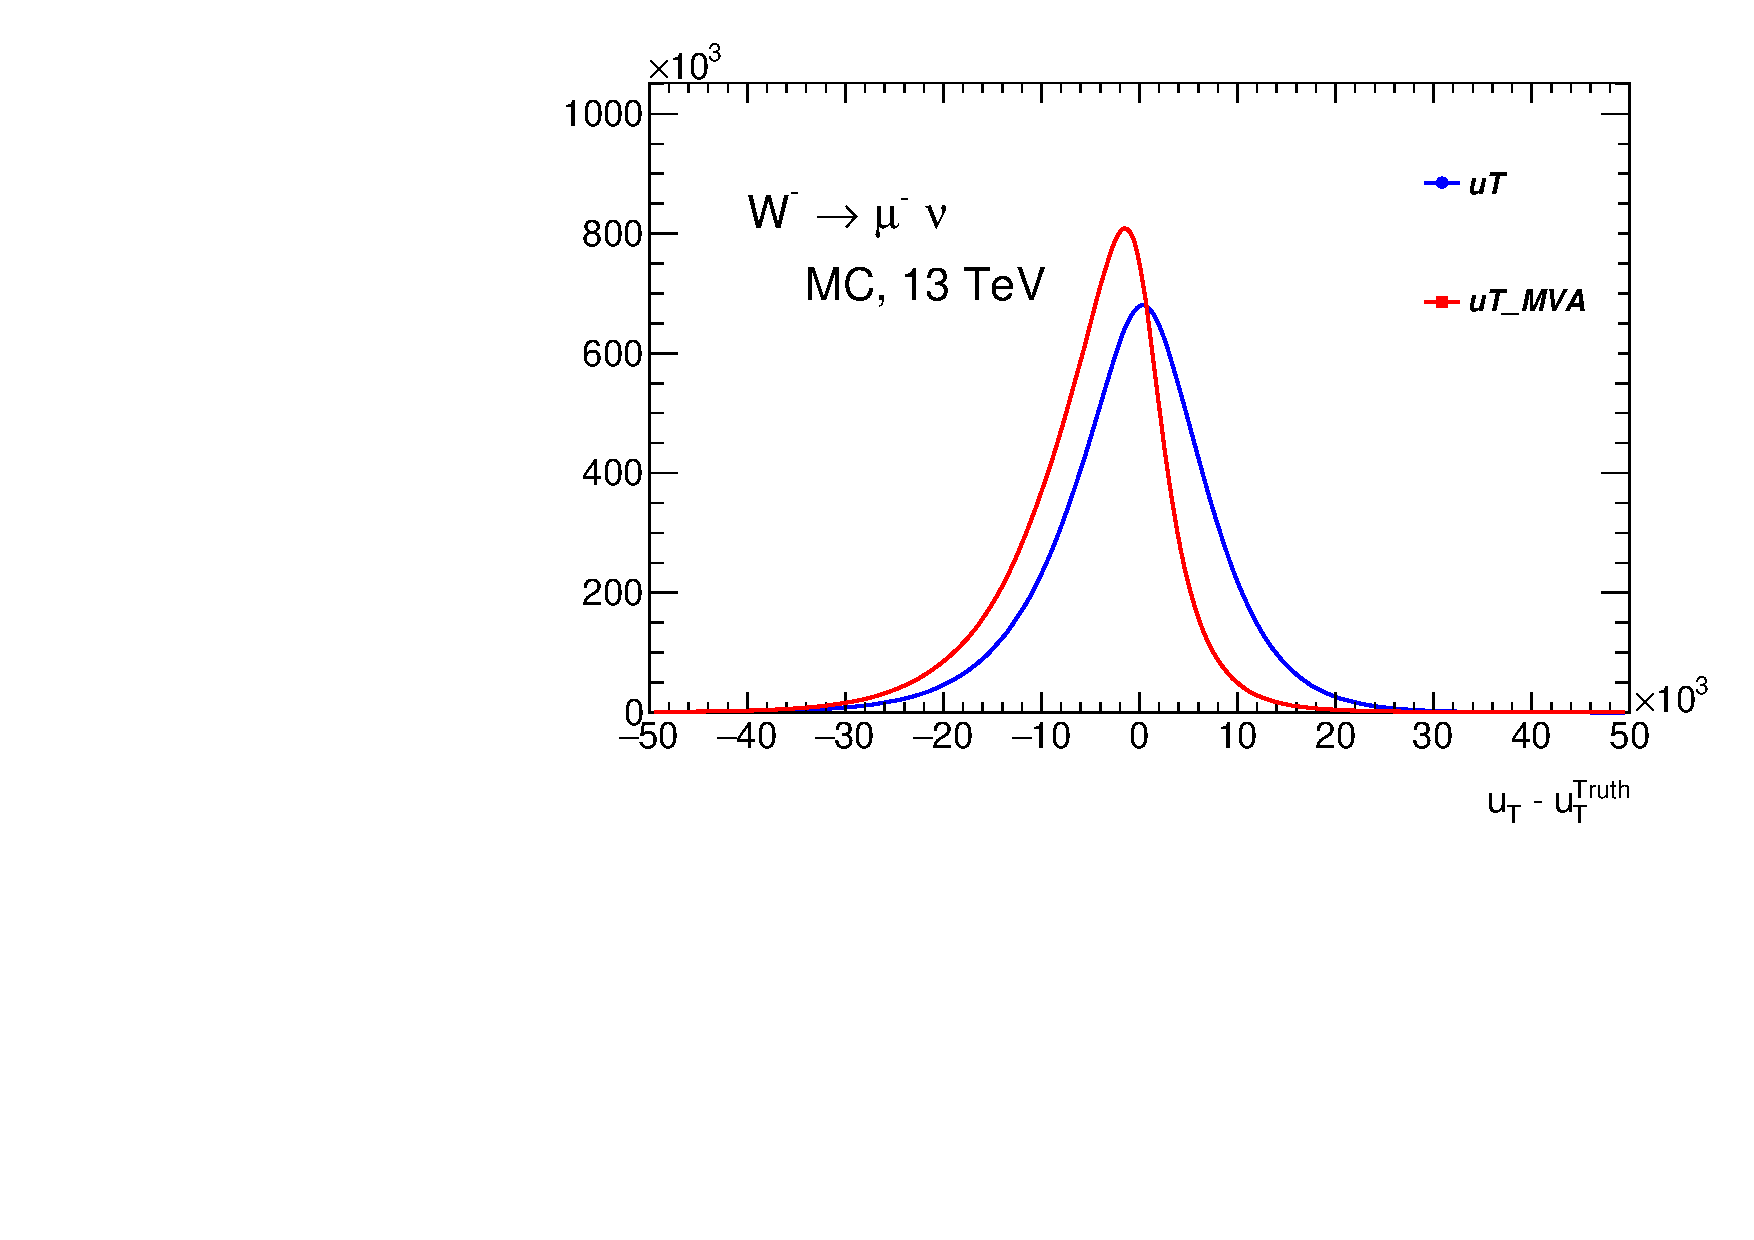
\includegraphics[width=.49\textwidth]{histosDeltaUtminusmunu.pdf}}
    	{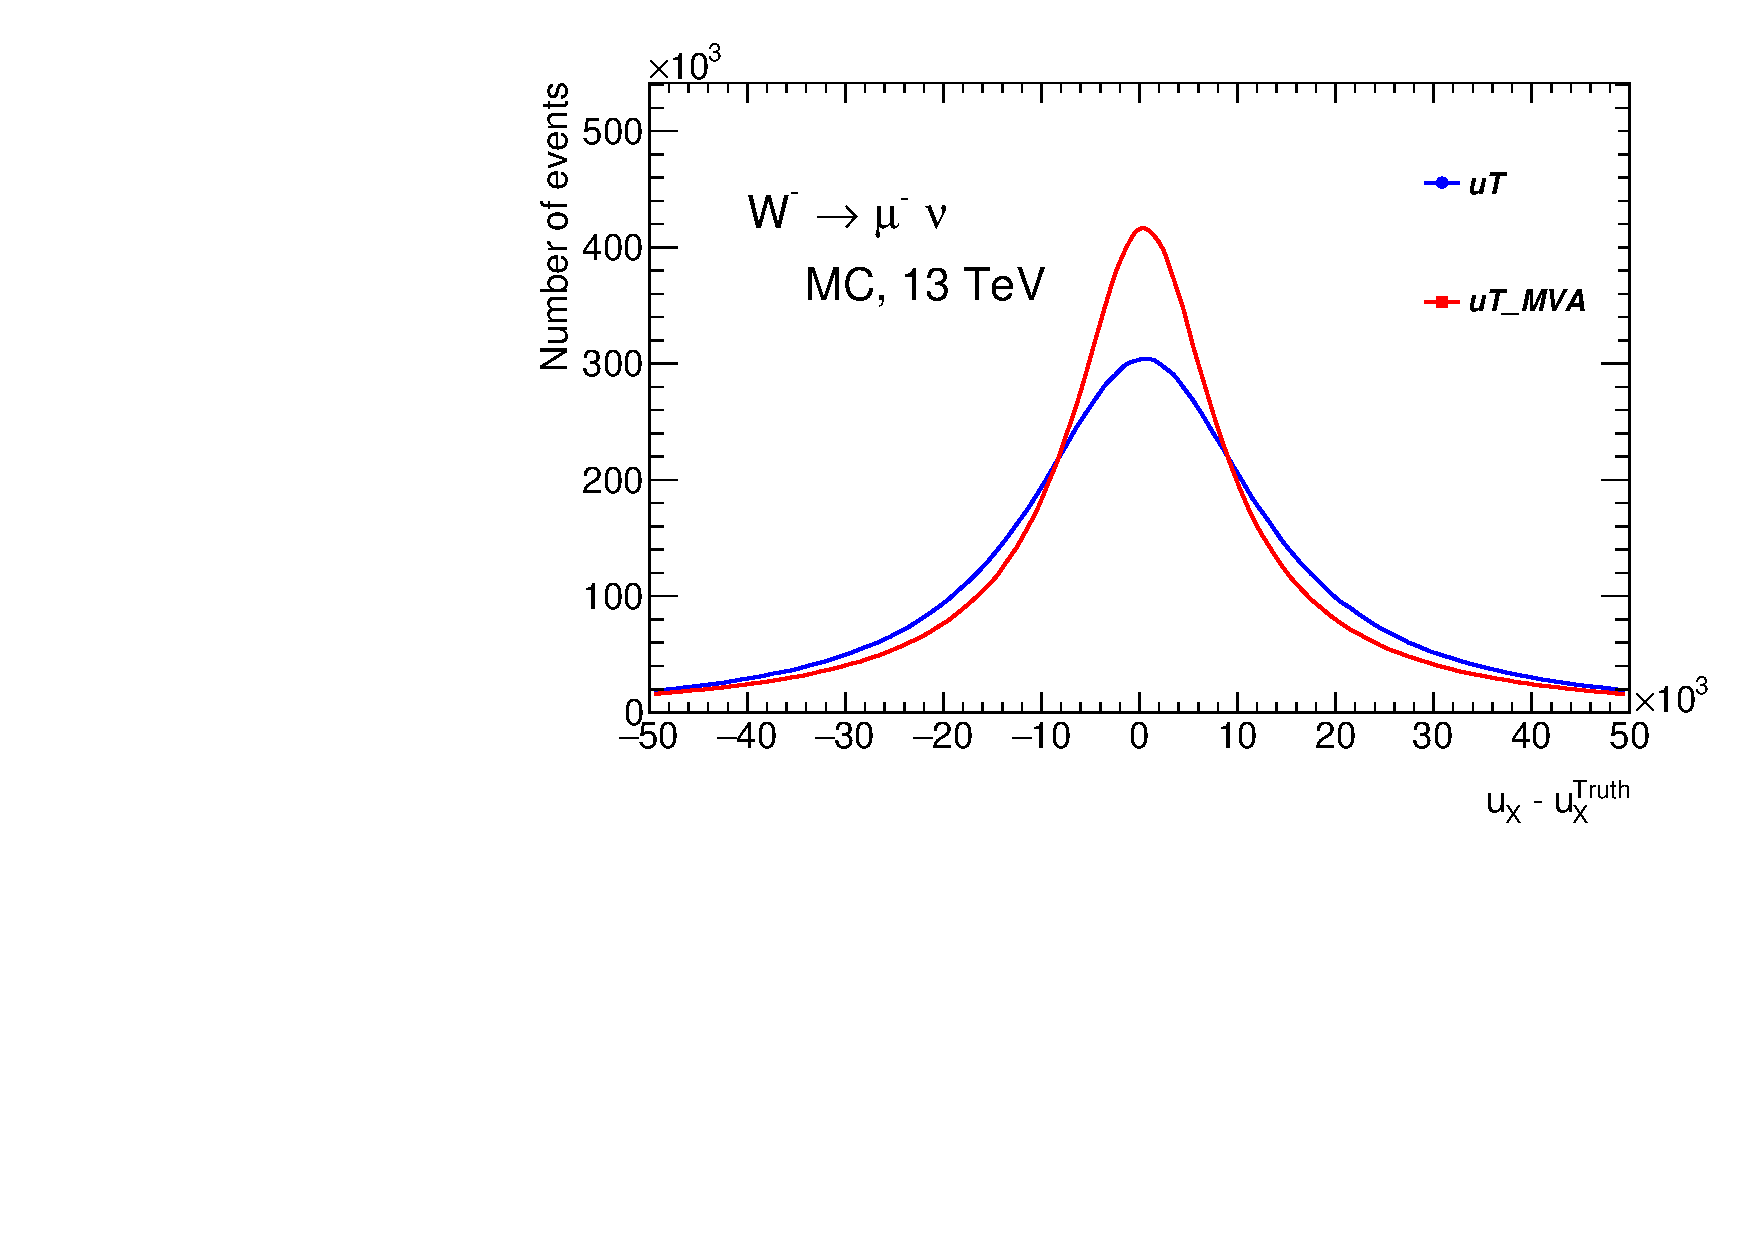
\includegraphics[width=.49\textwidth]{histosDeltaUxminusmunu.pdf}} \\
    	{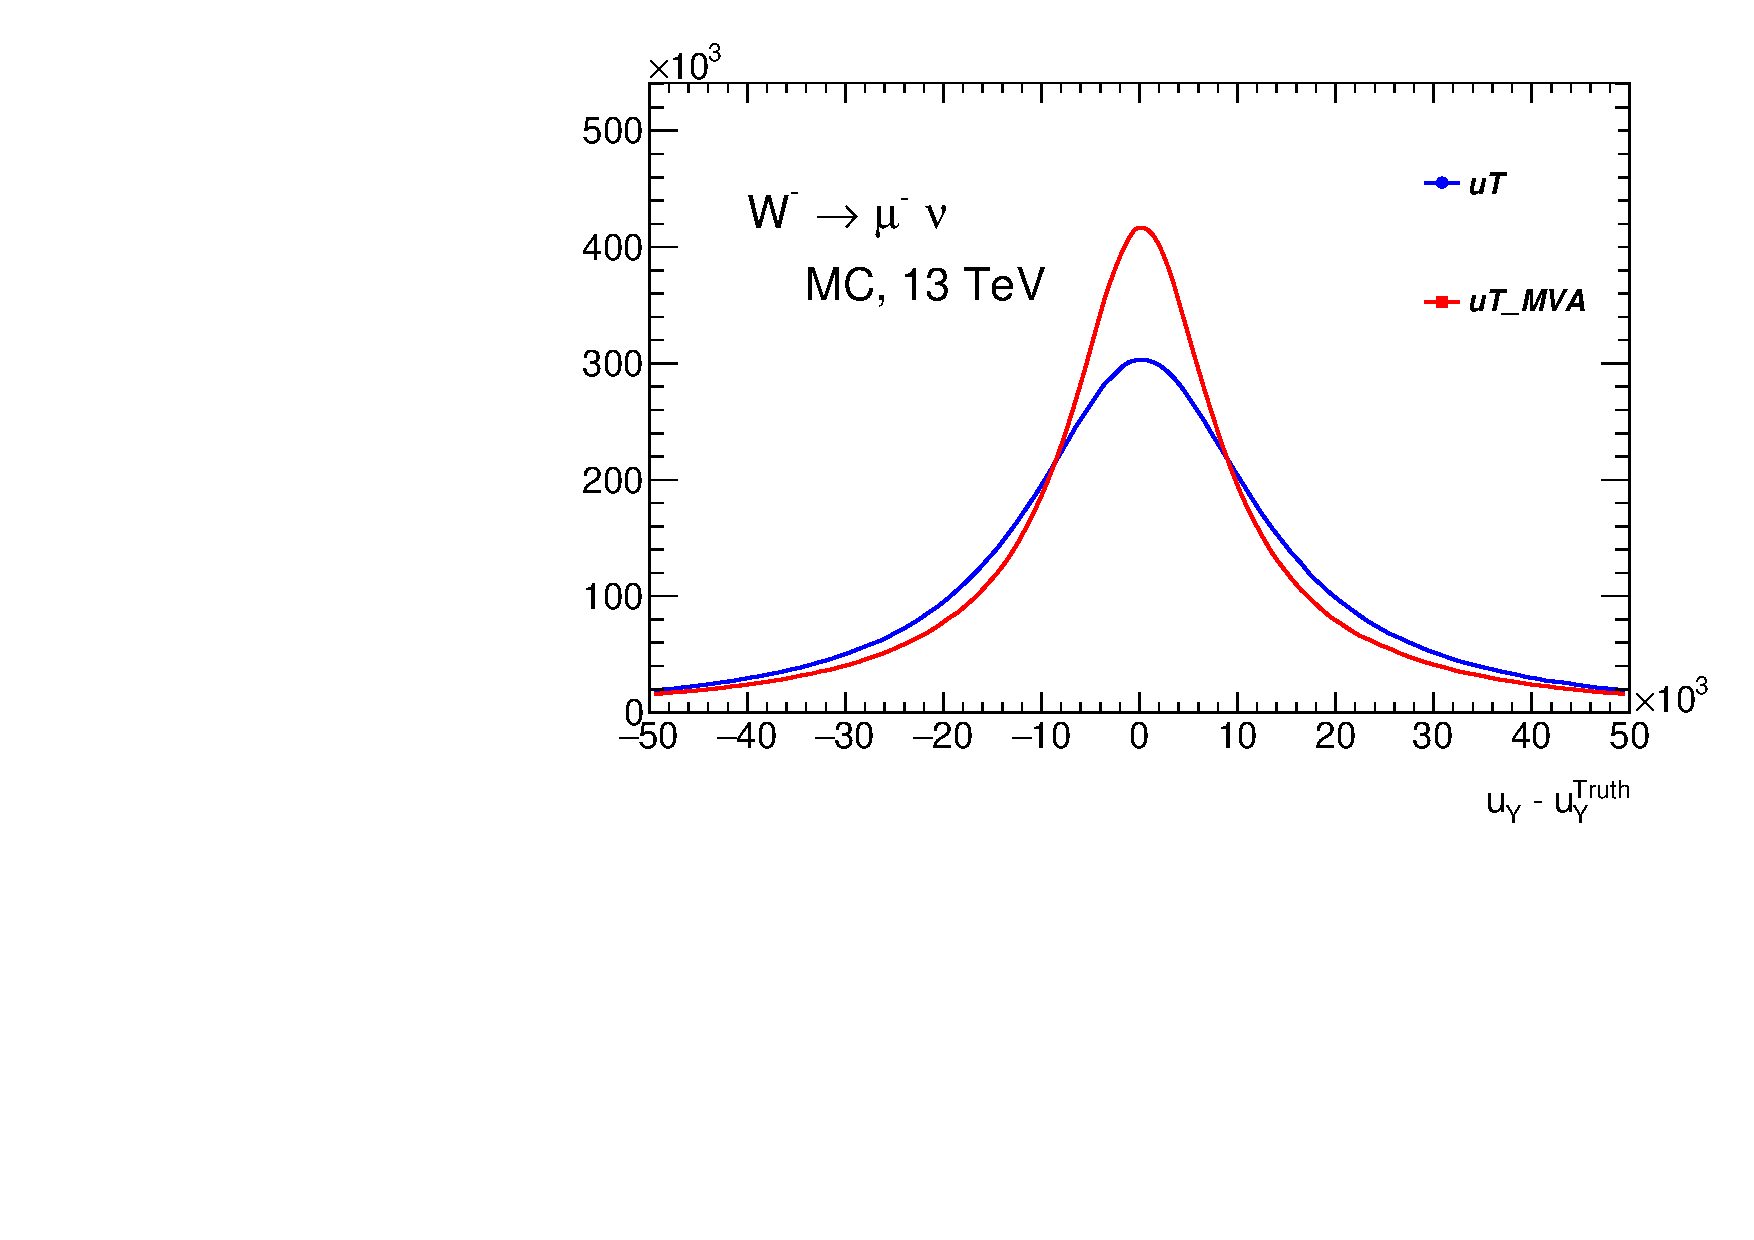
\includegraphics[width=.49\textwidth]{histosDeltaUyminusmunu.pdf}}
    	{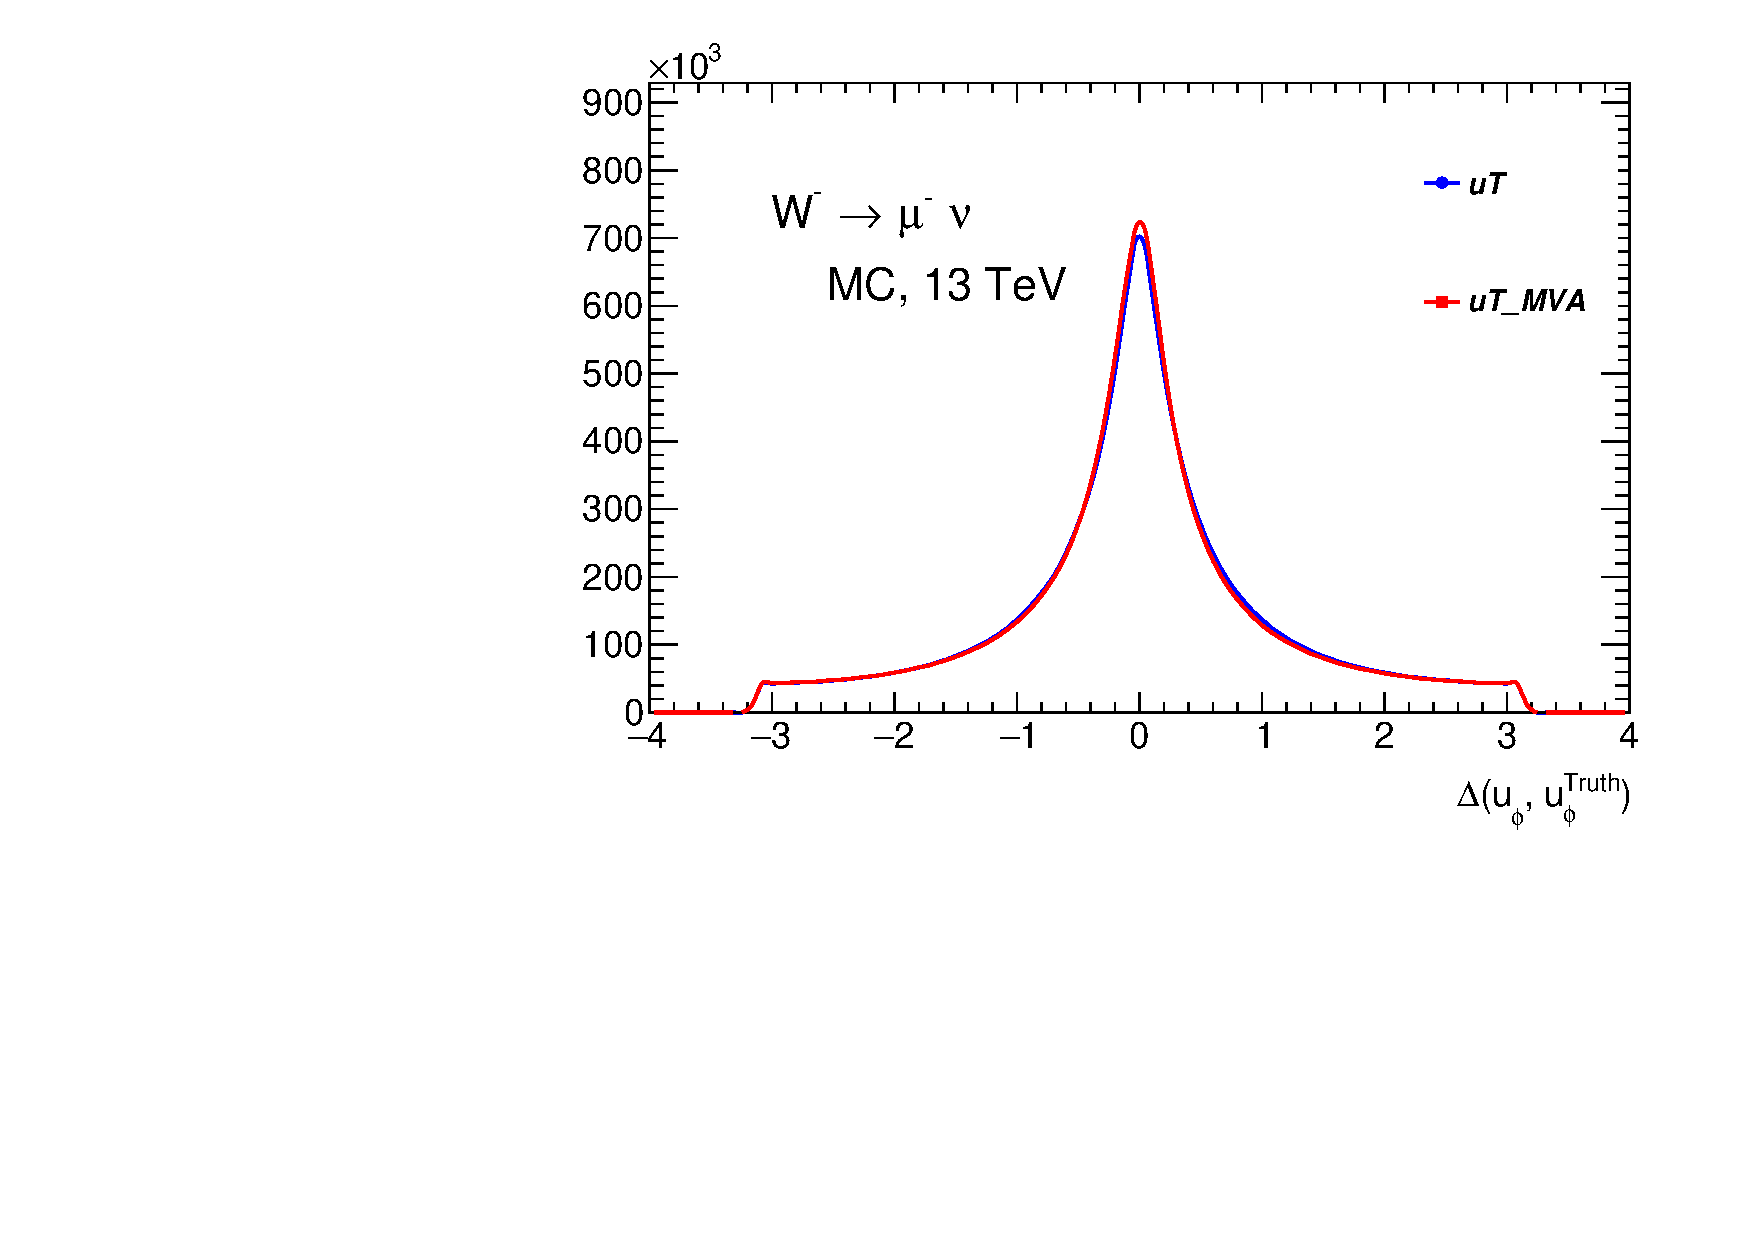
\includegraphics[width=.49\textwidth]{histosDeltaUPhiminusmunu.pdf}}\\
    	\label{fig:minusmunu_data_distributions1}
    \end{figure}
    \begin{figure}[h]
    	\centering
    	{\includegraphics[width=.49\textwidth]{outMVA_biasminusmunu}}
    	{\includegraphics[width=.49\textwidth]{outMVA_Uparminusmunu}}
    	{\includegraphics[width=.49\textwidth]{outMVA_uPerpminusmunu}}
    	{\includegraphics[width=.49\textwidth]{histosMeanBiasminusmunu}}
    	{\includegraphics[width=.49\textwidth]{histosSigmaUperpminusmunu}}
    	{\includegraphics[width=.49\textwidth]{histosUperpRelativeminusmunu}}
    	\caption{Comparison of kinematic distributions of $u_T$ vs $u_T^{MVA}$ for $W^-\rightarrow \mu^-\nu$ data sample.}
    	\label{fig:minusmunu_data_distributions2}
    \end{figure}
    
        
    \begin{figure}[h]
    	\centering
    	{\includegraphics[width=.49\textwidth]{hist_uXzmumumc.pdf}}
    	{\includegraphics[width=.49\textwidth]{hist_uYzmumumc.pdf}} \\
    	{\includegraphics[width=.49\textwidth]{hist_uTzmumumc.pdf}}
    	{\includegraphics[width=.49\textwidth]{hist_uPhizmumumc.pdf}}\\
    	{\includegraphics[width=.49\textwidth]{histosDeltaUtzmumumc.pdf}}
    	{\includegraphics[width=.49\textwidth]{histosDeltaUxzmumumc.pdf}} \\
    	{\includegraphics[width=.49\textwidth]{histosDeltaUyzmumumc.pdf}}
    	{\includegraphics[width=.49\textwidth]{histosDeltaUPhizmumumc.pdf}}\\
    	\label{fig:zmumu_mc_distributions1}
    \end{figure}
    \begin{figure}[h]
    	\centering
    	{\includegraphics[width=.49\textwidth]{outMVA_biaszmumumc}}
    	{\includegraphics[width=.49\textwidth]{outMVA_Uparzmumumc}}
    	{\includegraphics[width=.49\textwidth]{outMVA_uPerpzmumumc}}
    	{\includegraphics[width=.49\textwidth]{histosMeanBiaszmumumc}}
    	{\includegraphics[width=.49\textwidth]{histosSigmaUperpzmumumc}}
    	{\includegraphics[width=.49\textwidth]{histosUperpRelativezmumumc}}
    	\caption{Comparison of kinematic distributions of $u_T$ vs $u_T^{MVA}$ for $Z\rightarrow \mu\mu$ MC sample.}
    	\label{fig:zmumu_mc_distributions2}
    \end{figure}
    
    
    \begin{figure}[h]
    	\centering
    	{\includegraphics[width=.49\textwidth]{hist_uXzeemc.pdf}}
    	{\includegraphics[width=.49\textwidth]{hist_uYzeemc.pdf}} \\
    	{\includegraphics[width=.49\textwidth]{hist_uTzeemc.pdf}}
    	{\includegraphics[width=.49\textwidth]{hist_uPhizeemc.pdf}}\\
    	{\includegraphics[width=.49\textwidth]{histosDeltaUtzeemc.pdf}}
    	{\includegraphics[width=.49\textwidth]{histosDeltaUxzeemc.pdf}} \\
    	{\includegraphics[width=.49\textwidth]{histosDeltaUyzeemc.pdf}}
    	{\includegraphics[width=.49\textwidth]{histosDeltaUPhizeemc.pdf}}\\
    	\label{fig:zee_mc_distributions1}
    \end{figure}
    \begin{figure}[h]
    	\centering
    	{\includegraphics[width=.49\textwidth]{outMVA_biaszeemc}}
    	{\includegraphics[width=.49\textwidth]{outMVA_Uparzeemc}}
    	{\includegraphics[width=.49\textwidth]{outMVA_uPerpzeemc}}
    	{\includegraphics[width=.49\textwidth]{histosMeanBiaszeemc}}
    	{\includegraphics[width=.49\textwidth]{histosSigmaUperpzeemc}}
    	{\includegraphics[width=.49\textwidth]{histosUperpRelativezeemc}}
    	\caption{Comparison of kinematic distributions of $u_T$ vs $u_T^{MVA}$ for $Z\rightarrow ee$ MC sample.}
    	\label{fig:zee_mc_distributions2}
    \end{figure}


    \begin{figure}[h]
    	\centering
    	{\includegraphics[width=.49\textwidth]{hist_uXzmumudata.pdf}}
    	{\includegraphics[width=.49\textwidth]{hist_uYzmumudata.pdf}} \\
    	{\includegraphics[width=.49\textwidth]{hist_uTzmumudata.pdf}}
    	{\includegraphics[width=.49\textwidth]{hist_uPhizmumudata.pdf}}\\
    	{\includegraphics[width=.49\textwidth]{histosDeltaUtzmumudata.pdf}}
    	{\includegraphics[width=.49\textwidth]{histosDeltaUxzmumudata.pdf}} \\
    	{\includegraphics[width=.49\textwidth]{histosDeltaUyzmumudata.pdf}}
    	{\includegraphics[width=.49\textwidth]{histosDeltaUPhizmumudata.pdf}}\\
    	\label{fig:zmumu_data_distributions1}
    \end{figure}
    \begin{figure}[h]
    	\centering
    	{\includegraphics[width=.49\textwidth]{outMVA_biaszmumudata}}
    	{\includegraphics[width=.49\textwidth]{outMVA_Uparzmumudata}}
    	{\includegraphics[width=.49\textwidth]{outMVA_uPerpzmumudata}}
    	{\includegraphics[width=.49\textwidth]{histosMeanBiaszmumudata}}
    	{\includegraphics[width=.49\textwidth]{histosSigmaUperpzmumudata}}
    	{\includegraphics[width=.49\textwidth]{histosUperpRelativezmumudata}}
    	\caption{Comparison of kinematic distributions of $u_T$ vs $u_T^{MVA}$ for $Z\rightarrow \mu\mu$ data sample.}
    	\label{fig:zmumu_data_distributions2}
    \end{figure}
    
    
\begin{figure}[h]
	\centering
	{\includegraphics[width=.49\textwidth]{hist_uXzeedata.pdf}}
	{\includegraphics[width=.49\textwidth]{hist_uYzeedata.pdf}} \\
	{\includegraphics[width=.49\textwidth]{hist_uTzeedata.pdf}}
	{\includegraphics[width=.49\textwidth]{hist_uPhizeedata.pdf}}\\
	{\includegraphics[width=.49\textwidth]{histosDeltaUtzeedata.pdf}}
	{\includegraphics[width=.49\textwidth]{histosDeltaUxzeedata.pdf}} \\
	{\includegraphics[width=.49\textwidth]{histosDeltaUyzeedata.pdf}}
	{\includegraphics[width=.49\textwidth]{histosDeltaUPhizeedata.pdf}}\\
	\label{fig:zee_data_distributions1}
\end{figure}
\begin{figure}[h]
	\centering
	{\includegraphics[width=.49\textwidth]{outMVA_biaszeedata}}
	{\includegraphics[width=.49\textwidth]{outMVA_Uparzeedata}}
	{\includegraphics[width=.49\textwidth]{outMVA_uPerpzeedata}}
	{\includegraphics[width=.49\textwidth]{histosMeanBiaszeedata}}
	{\includegraphics[width=.49\textwidth]{histosSigmaUperpzeedata}}
	{\includegraphics[width=.49\textwidth]{histosUperpRelativezeedata}}
	\caption{Comparison of kinematic distributions of $u_T$ vs $u_T^{MVA}$ for $Z\rightarrow ee$ data sample.}
	\label{fig:zee_data_distributions2}
\end{figure}
%
%
